\documentclass{article}
\usepackage{graphicx}
\usepackage{float}
\usepackage{subcaption}
\usepackage{geometry}
\usepackage{hyperref}

\geometry{a4paper, margin=1in}

\title{t-SNE Visualization Report: Partial Discharge Data}
\author{}
\date{\today}

\begin{document}

\maketitle

\begin{abstract}
This report documents the t-SNE dimensionality reduction visualizations performed on the Partial Discharge (PD) dataset. The data representations are analyzed across two primary categorization structures: \texttt{data\_by\_type} (grouped directly by PD defect type) and \texttt{data\_by\_date} (organized chronologically by Lab/Field collection context). A 256-dimensional feature vector was extracted from the raw Phase-Resolved Partial Discharge (PRPD) matrices for each sample and projected into 2D and 3D spaces.
\end{abstract}

\section{Visualizations: Data Organized by Type}
This section illustrates the dataset strictly categorized by discharge type. The global cluster shows all classes together, followed by split graphs highlighting individual classes (Corona, Floating, Particle, Void, and Noise) against the background manifold.

\subsection{Global Clusters (Data by Type)}
\begin{figure}[H]
    \centering
    \begin{subfigure}[b]{0.45\textwidth}
        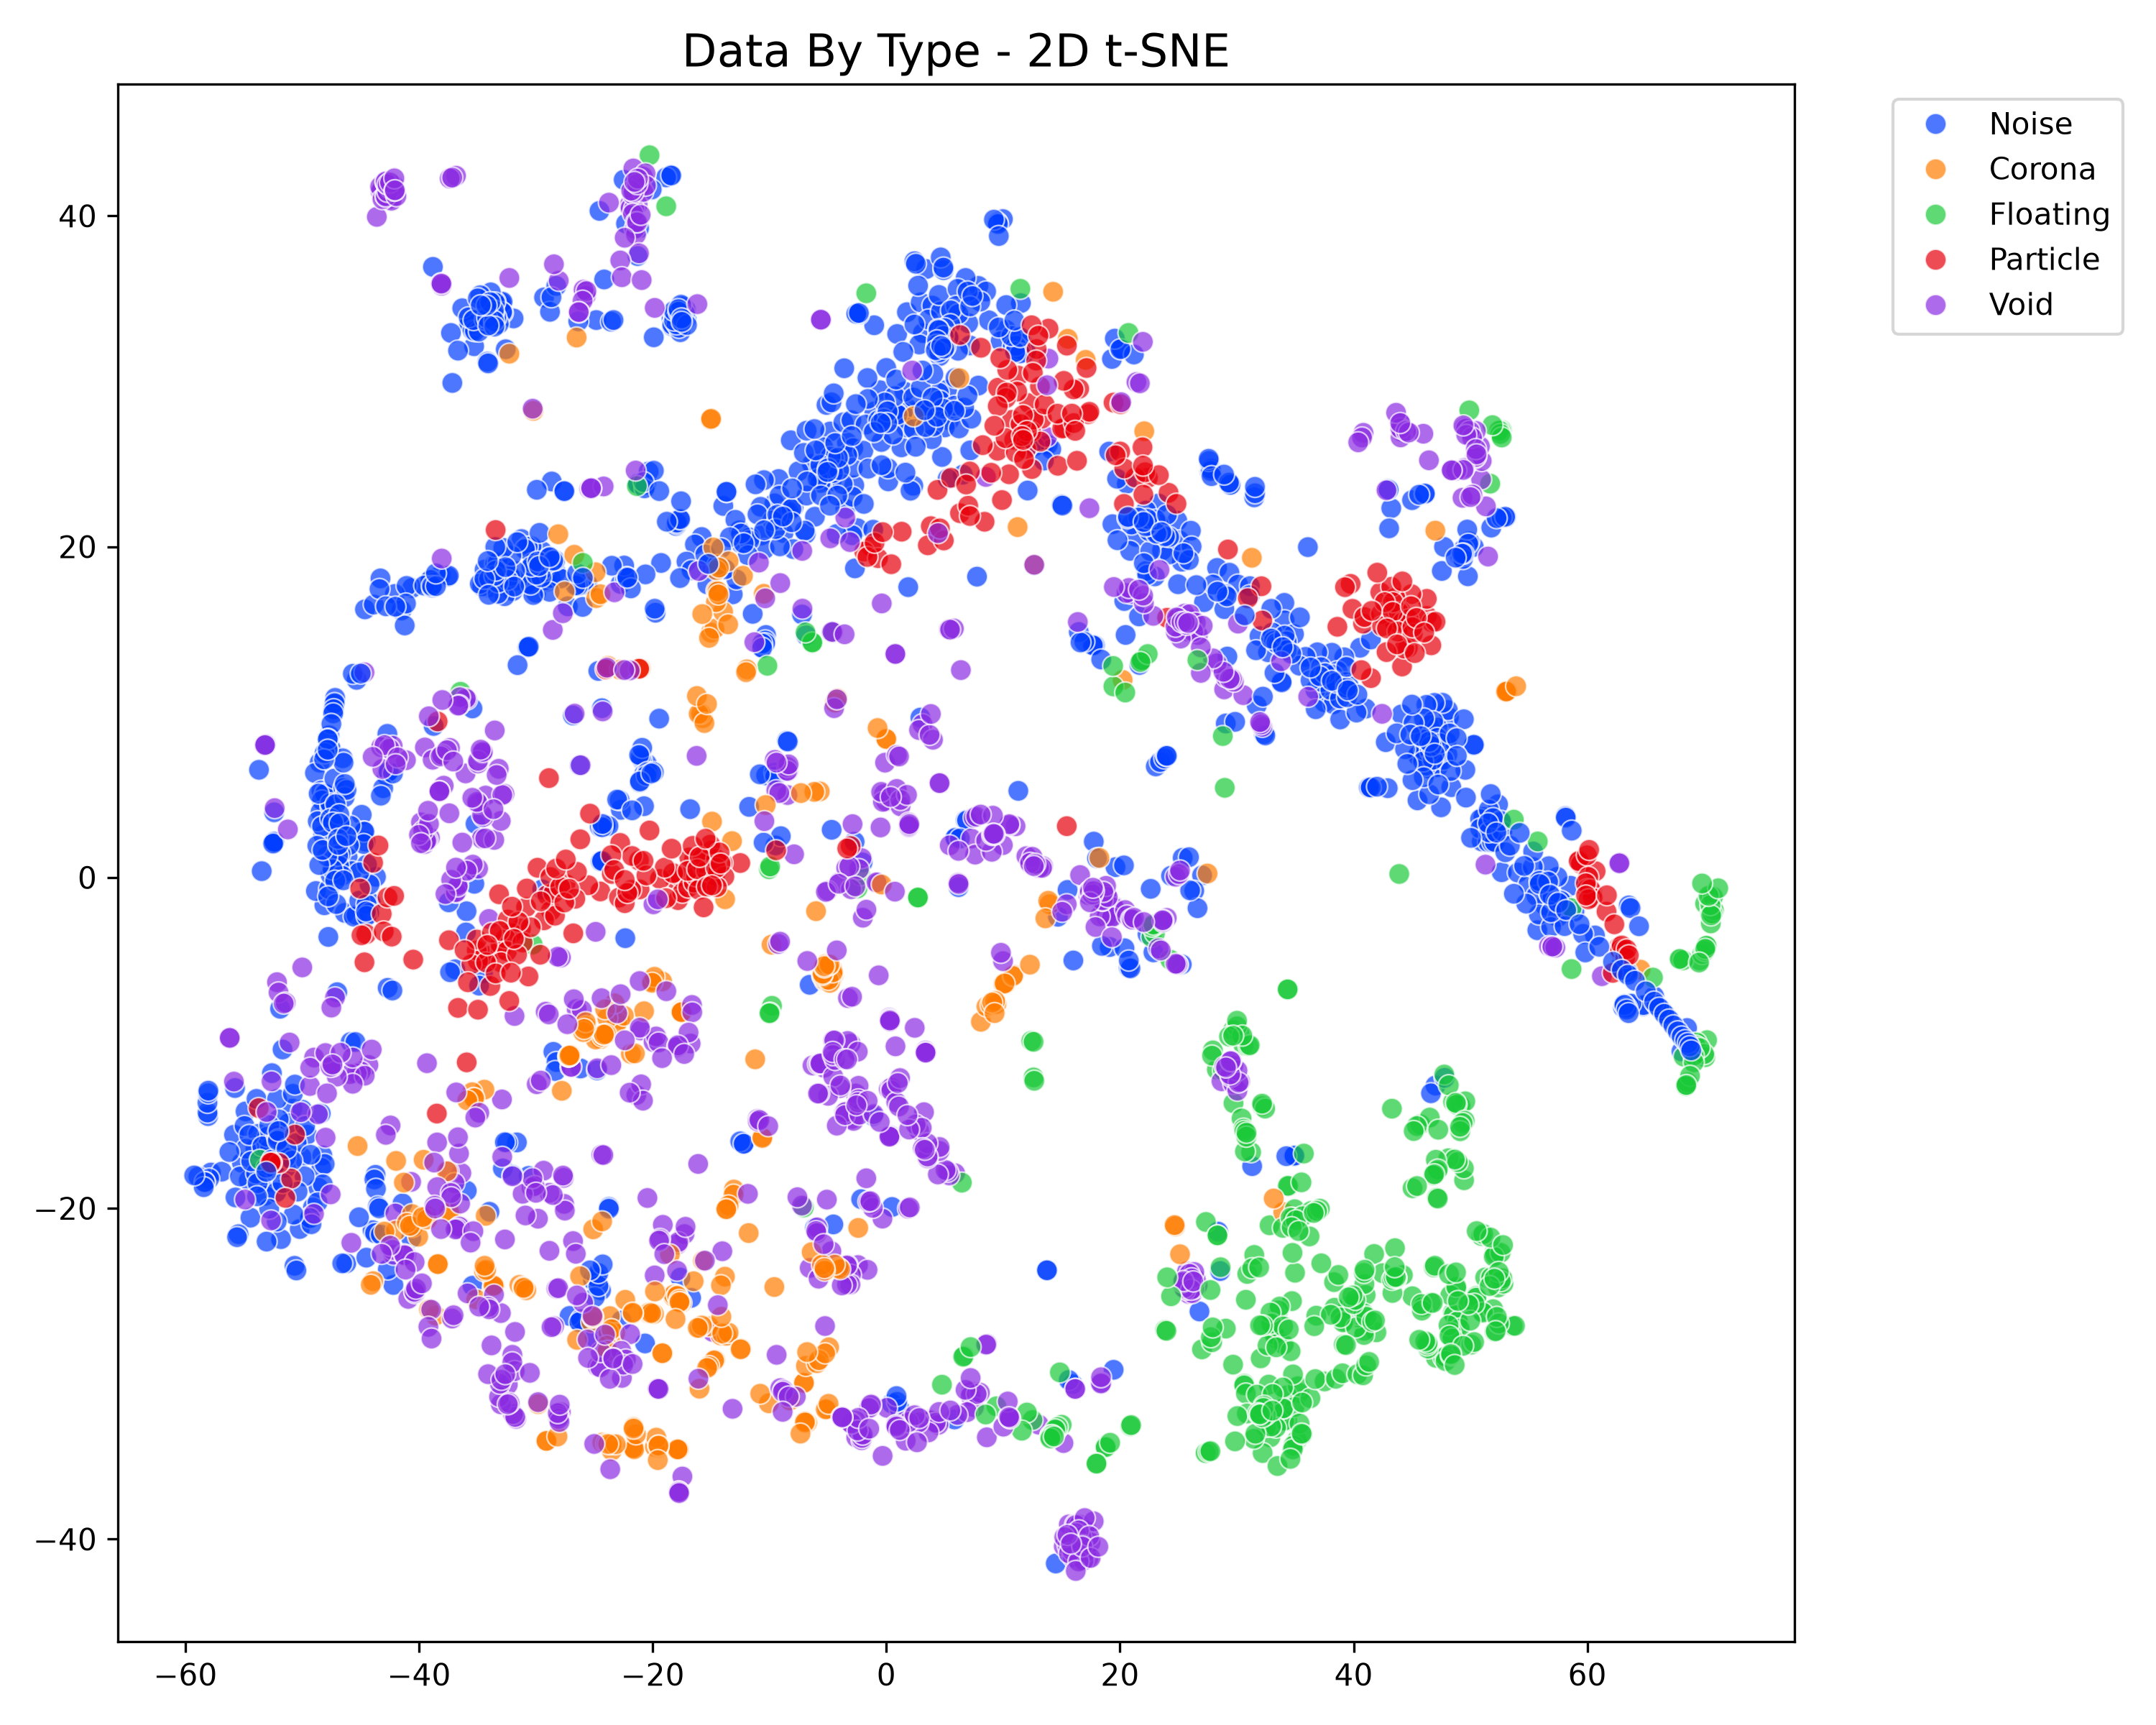
\includegraphics[width=\textwidth]{../Results/tsne_plots/data_by_type/2d_plot.png}
        \caption{Global 2D t-SNE}
    \end{subfigure}
    \hfill
    \begin{subfigure}[b]{0.45\textwidth}
        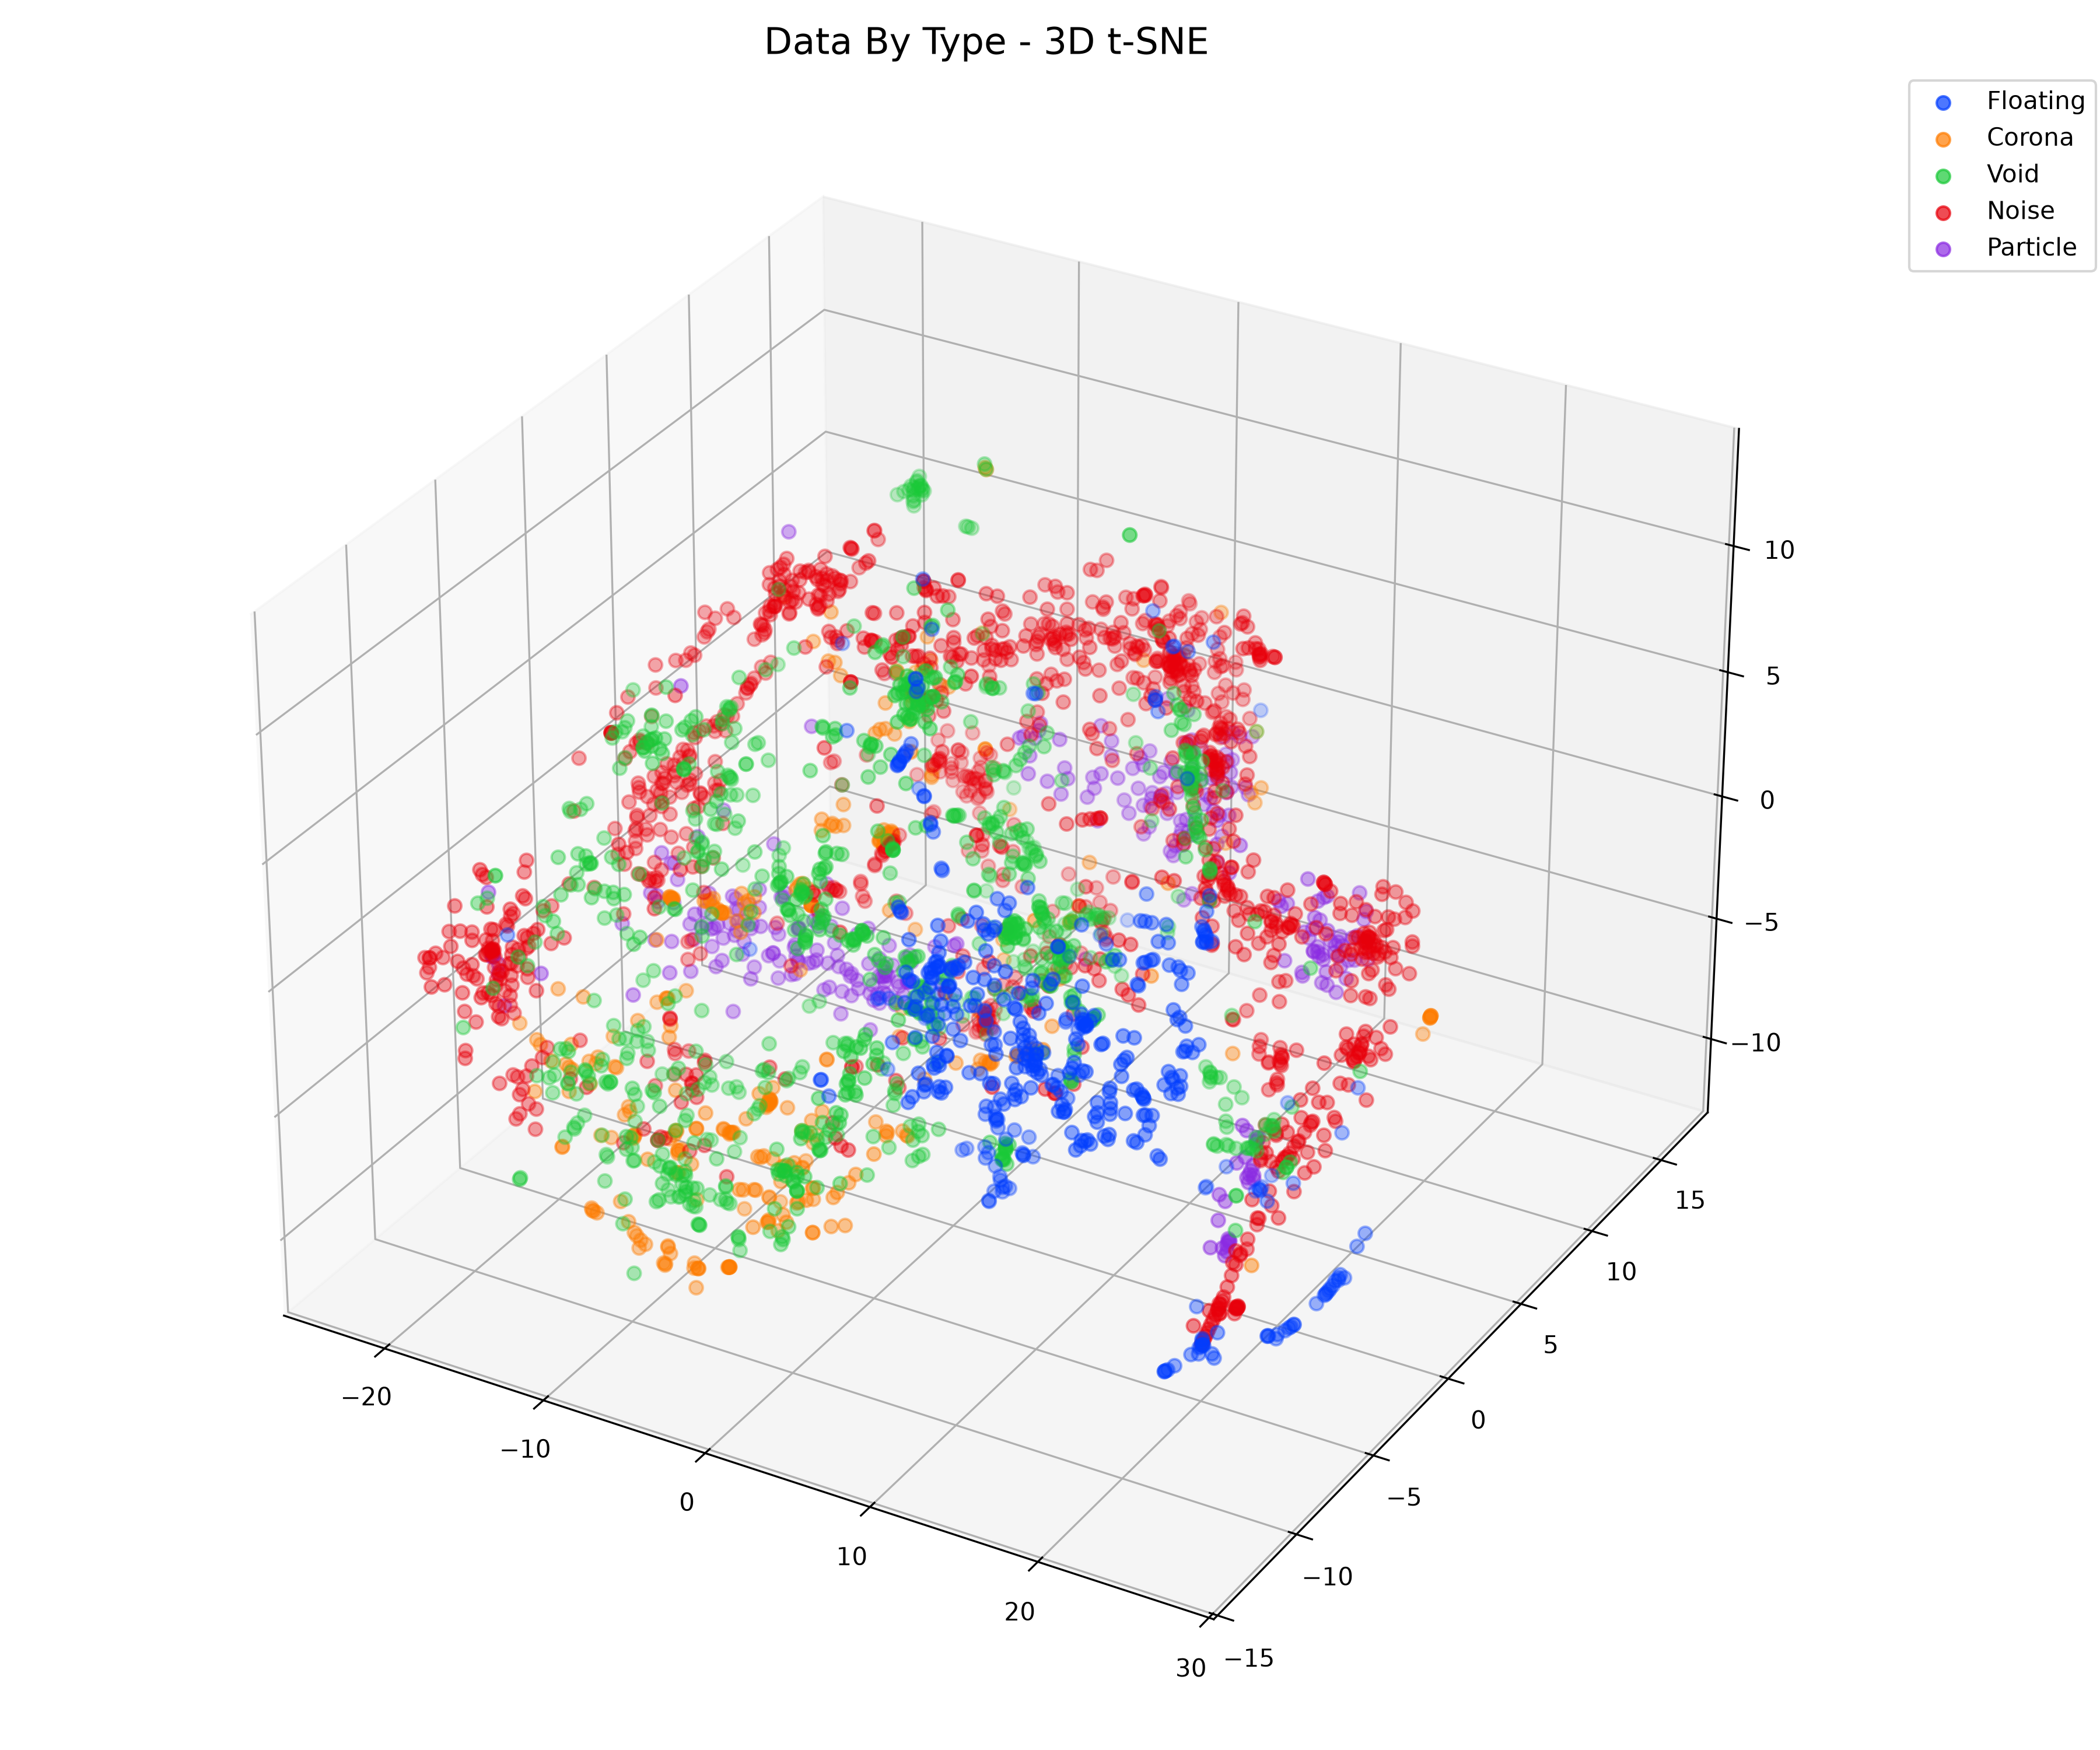
\includegraphics[width=\textwidth]{../Results/tsne_plots/data_by_type/3d_plot.png}
        \caption{Global 3D t-SNE}
    \end{subfigure}
    \caption{Global t-SNE projections for all classes in \texttt{data\_by\_type}.}
\end{figure}

\subsection{Class-Specific Projections (Data by Type)}

% Corona
\begin{figure}[H]
    \centering
    \begin{subfigure}[b]{0.45\textwidth}
        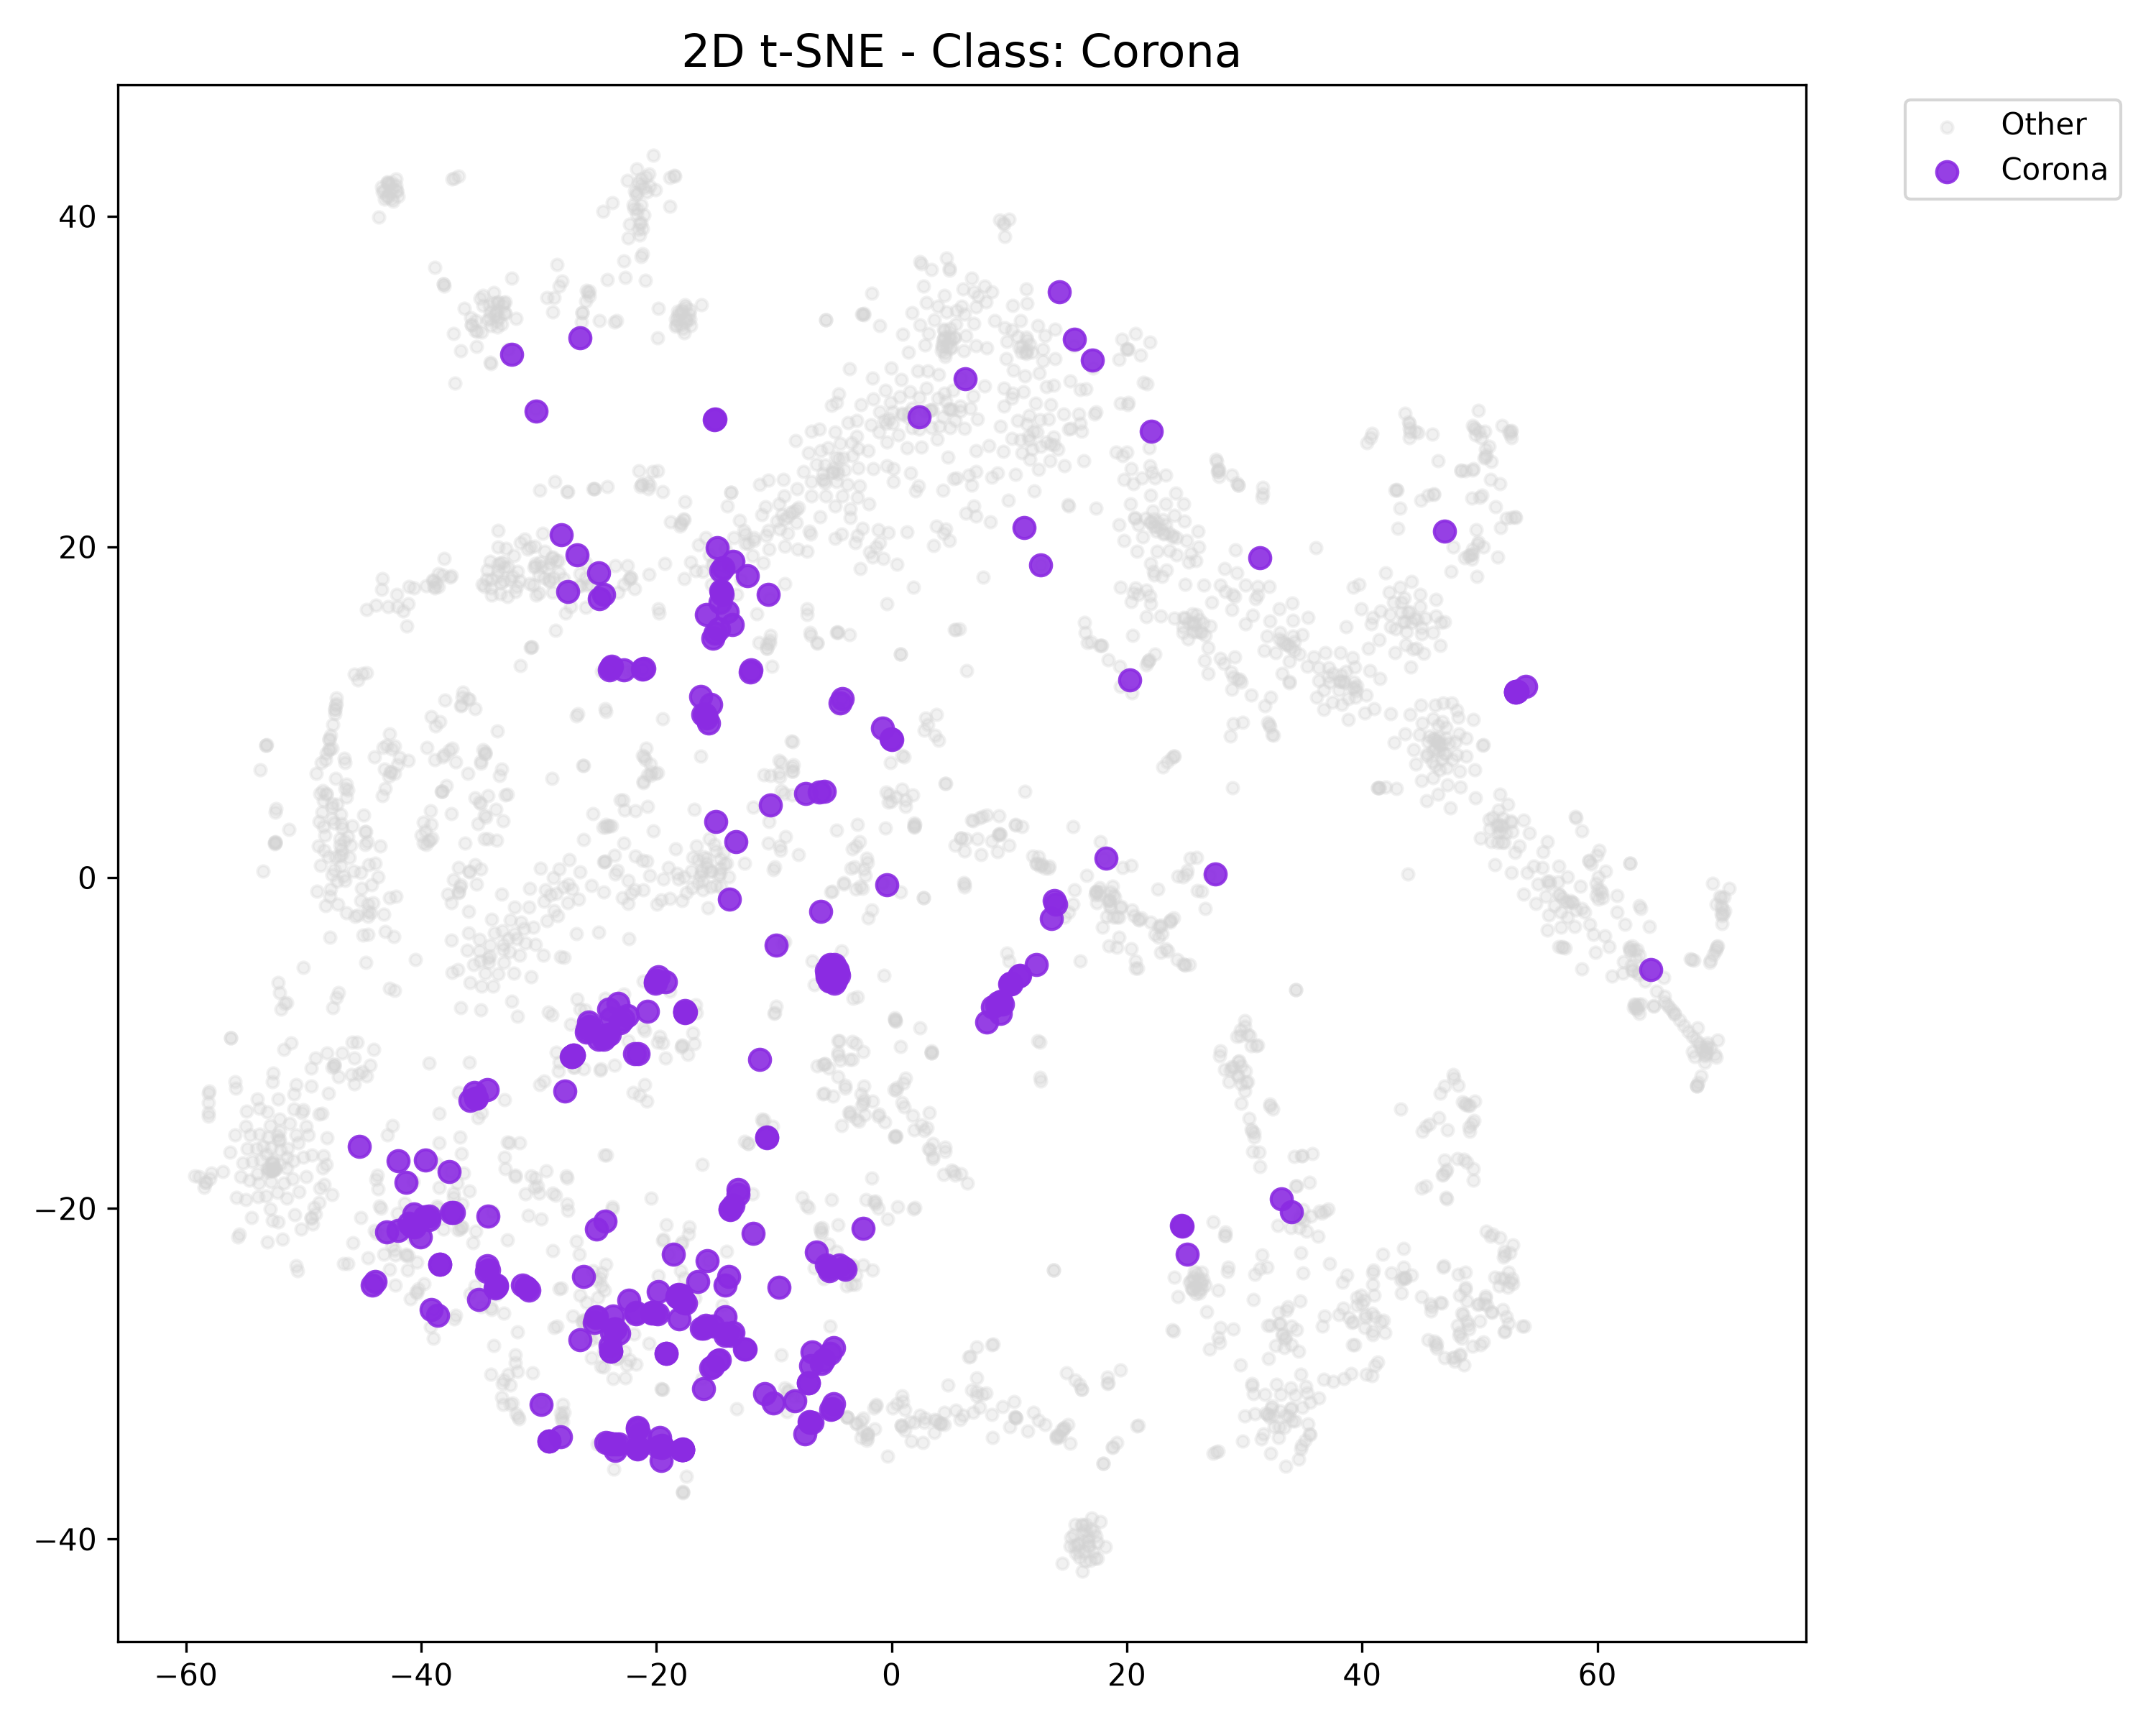
\includegraphics[width=\textwidth]{../Results/tsne_plots/data_by_type/split_2d_Corona.png}
        \caption{2D t-SNE: Corona}
    \end{subfigure}
    \hfill
    \begin{subfigure}[b]{0.45\textwidth}
        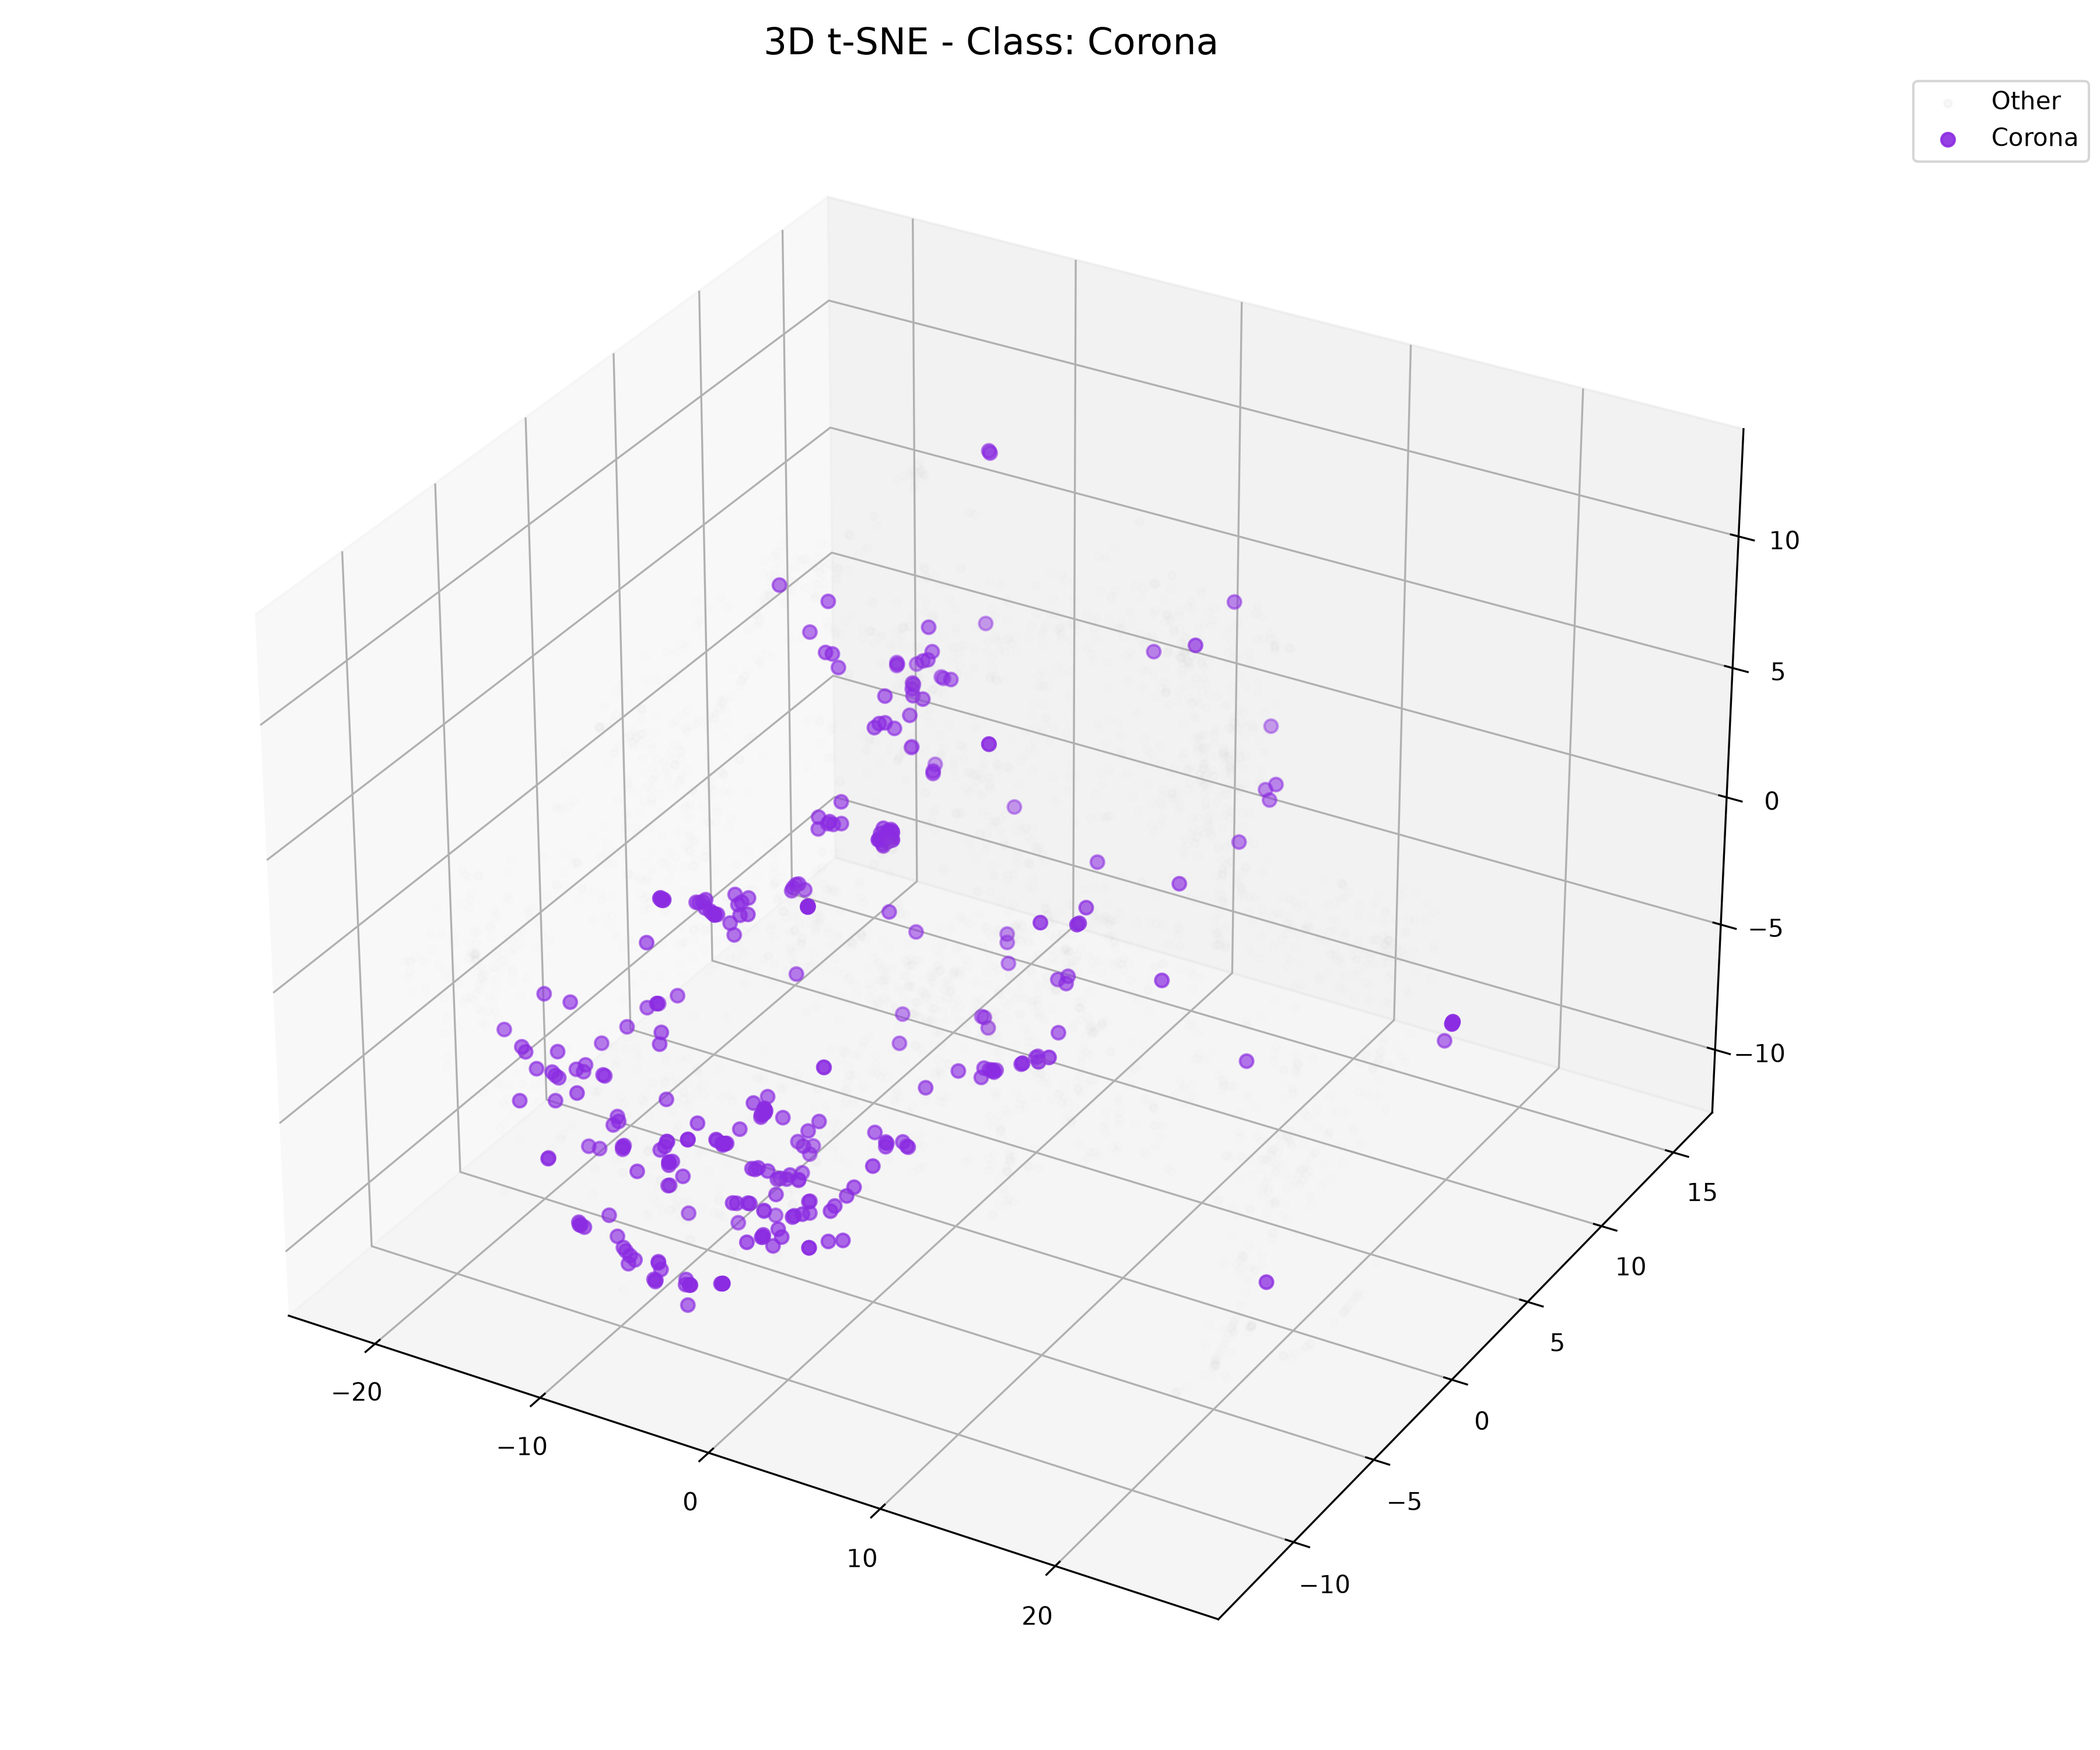
\includegraphics[width=\textwidth]{../Results/tsne_plots/data_by_type/split_3d_Corona.png}
        \caption{3D t-SNE: Corona}
    \end{subfigure}
    \caption{Highlighted distribution of Corona discharges.}
\end{figure}

% Floating
\begin{figure}[H]
    \centering
    \begin{subfigure}[b]{0.45\textwidth}
        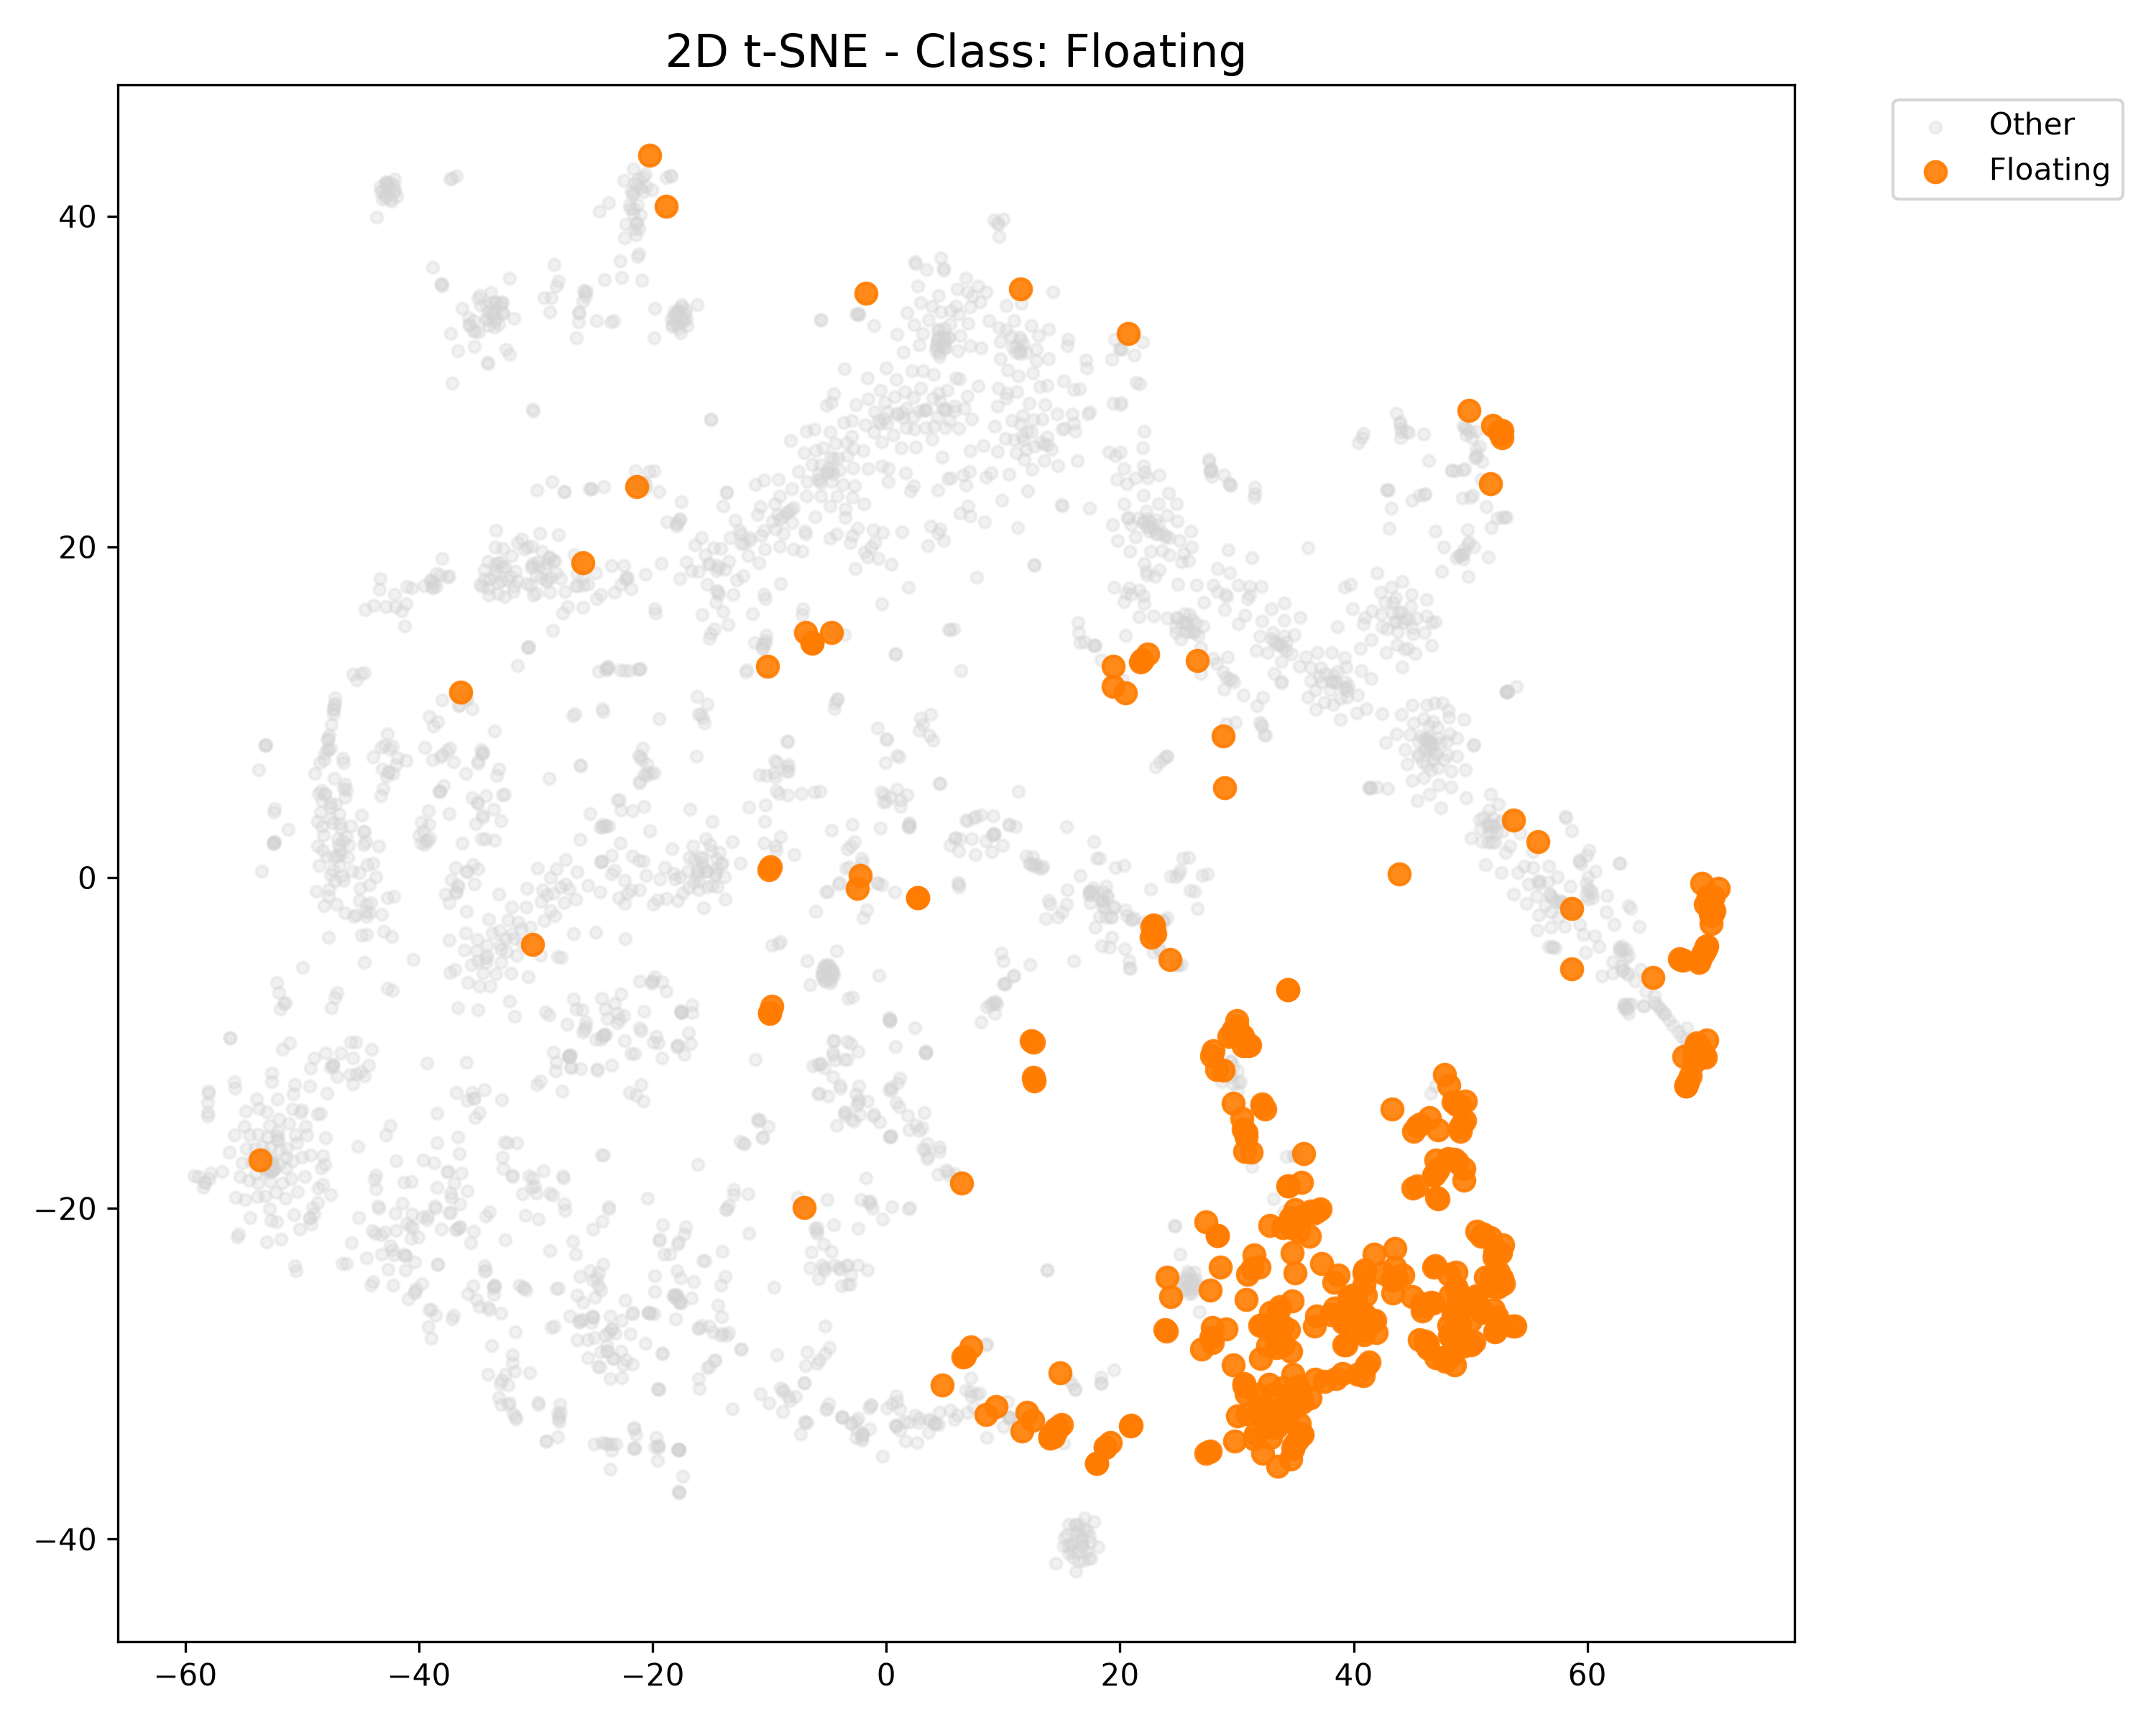
\includegraphics[width=\textwidth]{../Results/tsne_plots/data_by_type/split_2d_Floating.png}
        \caption{2D t-SNE: Floating}
    \end{subfigure}
    \hfill
    \begin{subfigure}[b]{0.45\textwidth}
        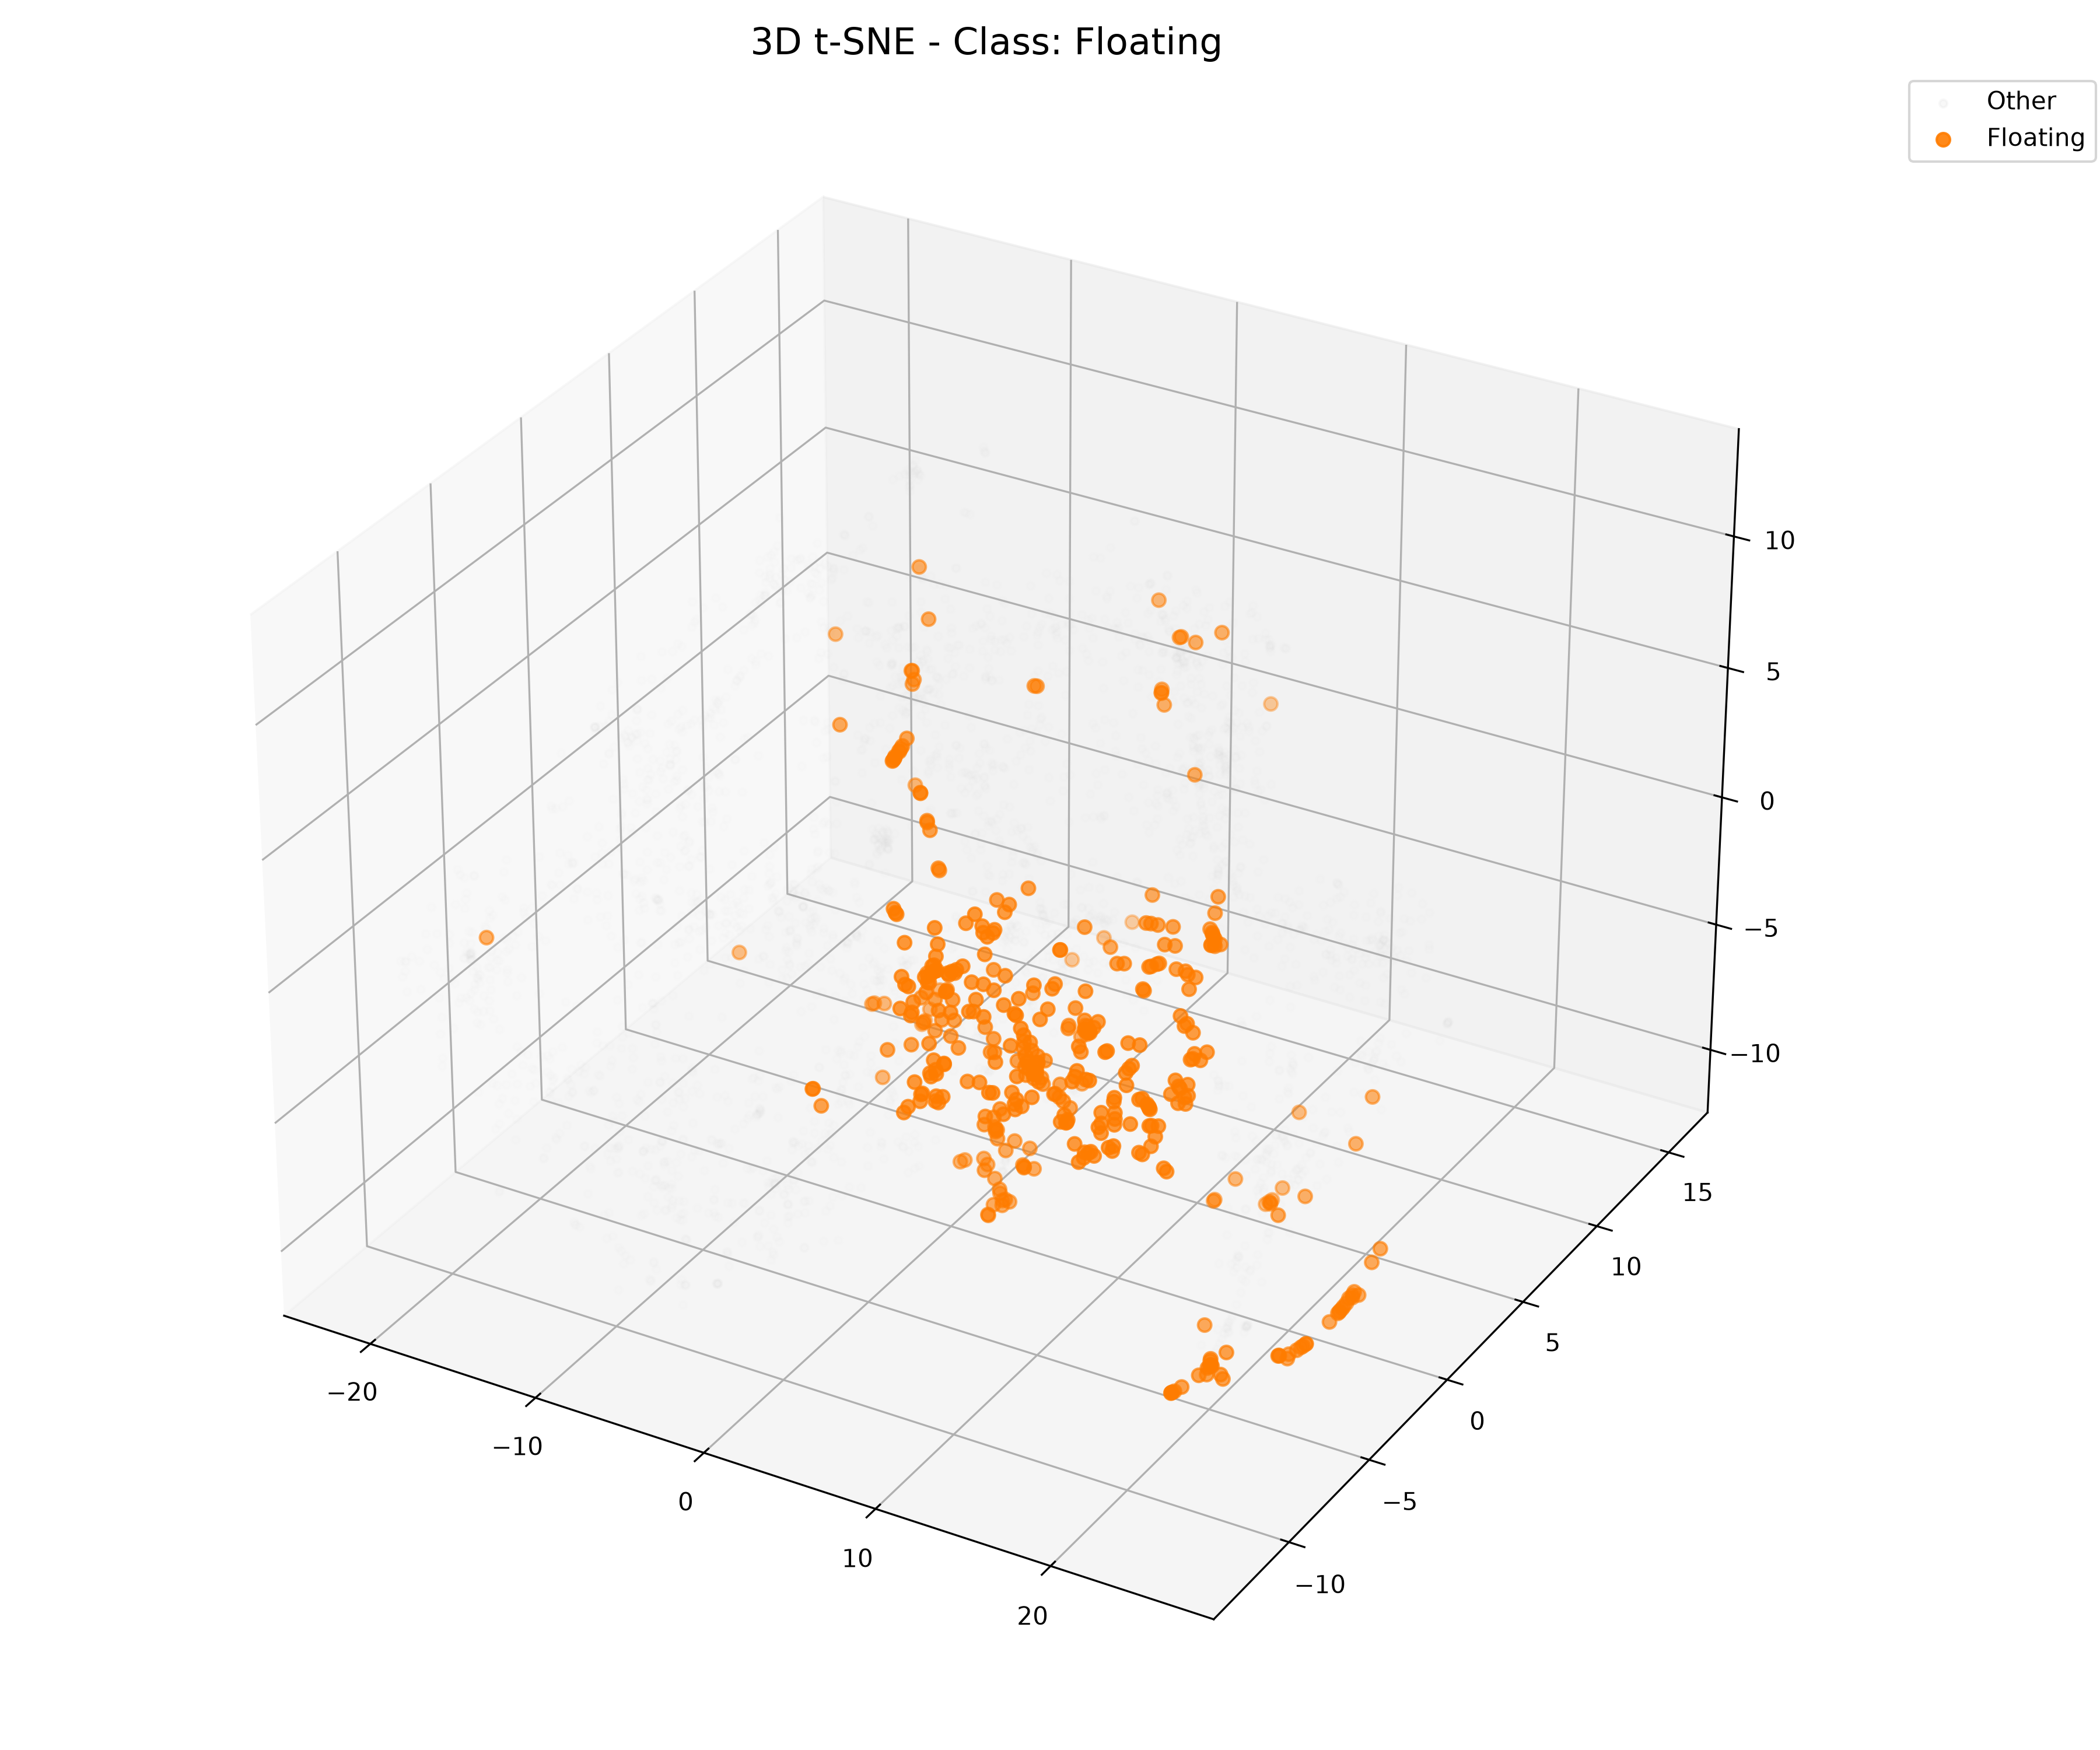
\includegraphics[width=\textwidth]{../Results/tsne_plots/data_by_type/split_3d_Floating.png}
        \caption{3D t-SNE: Floating}
    \end{subfigure}
    \caption{Highlighted distribution of Floating discharges.}
\end{figure}

% Particle
\begin{figure}[H]
    \centering
    \begin{subfigure}[b]{0.45\textwidth}
        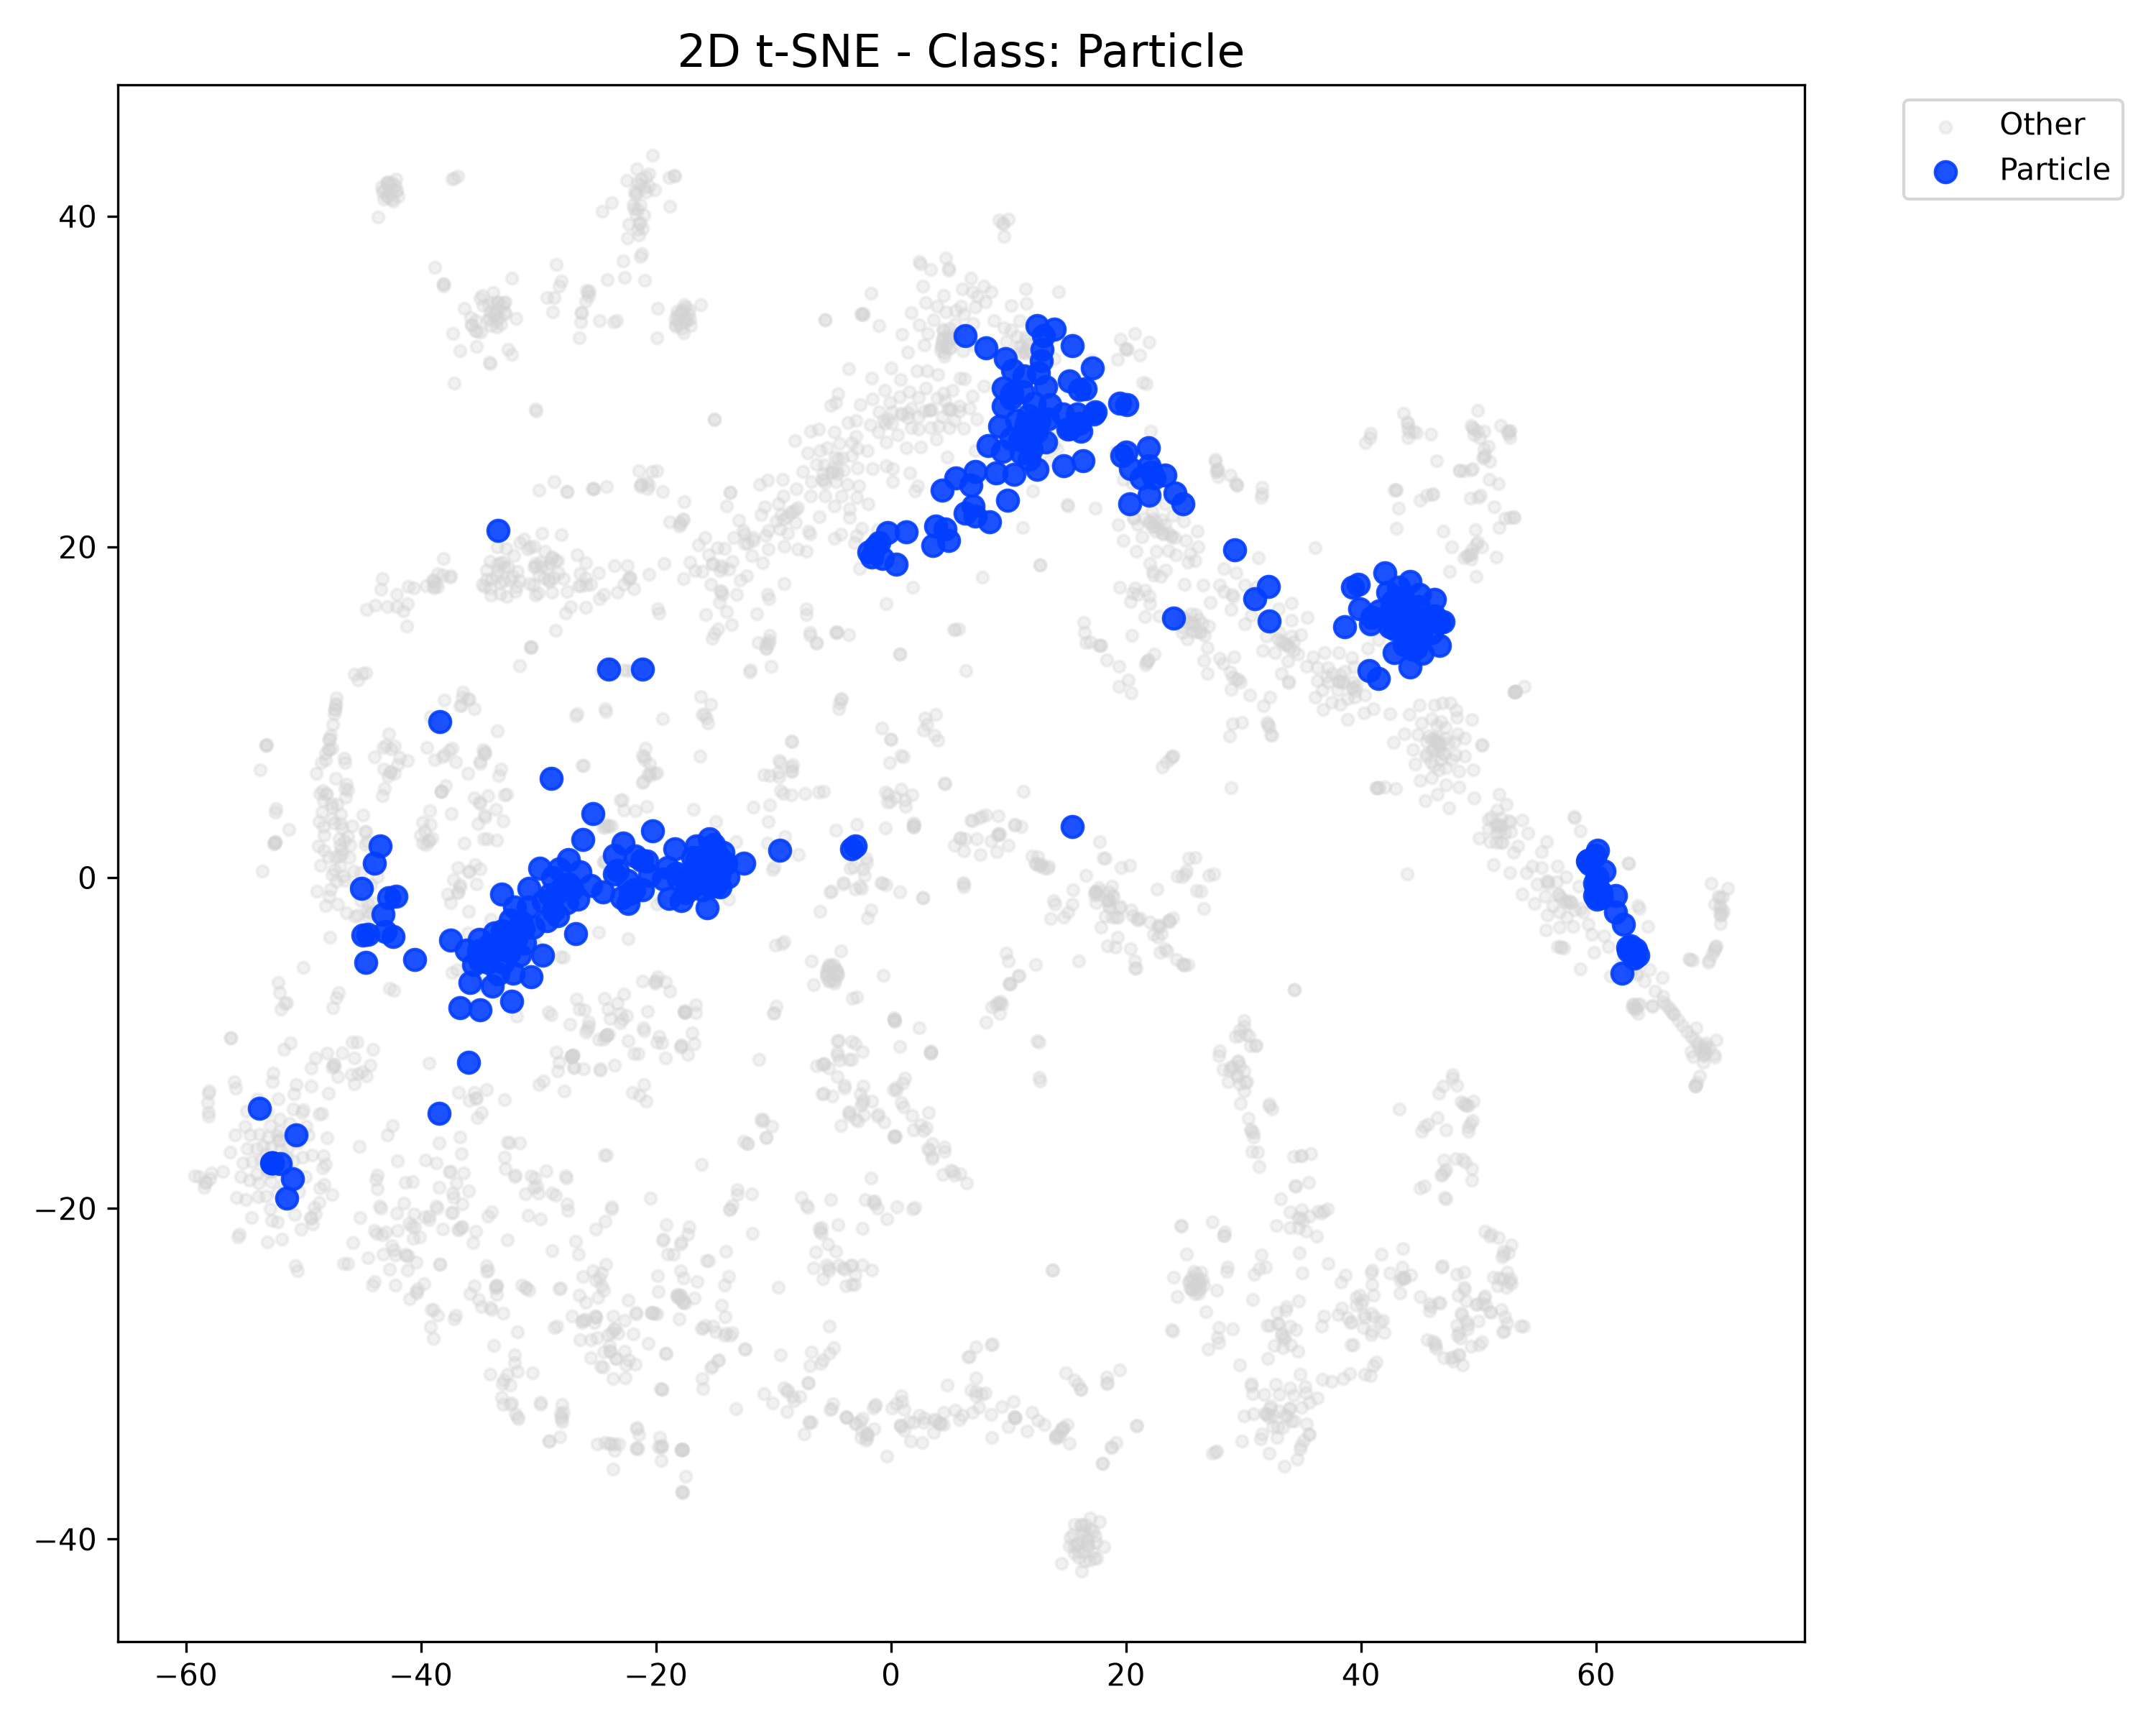
\includegraphics[width=\textwidth]{../Results/tsne_plots/data_by_type/split_2d_Particle.png}
        \caption{2D t-SNE: Particle}
    \end{subfigure}
    \hfill
    \begin{subfigure}[b]{0.45\textwidth}
        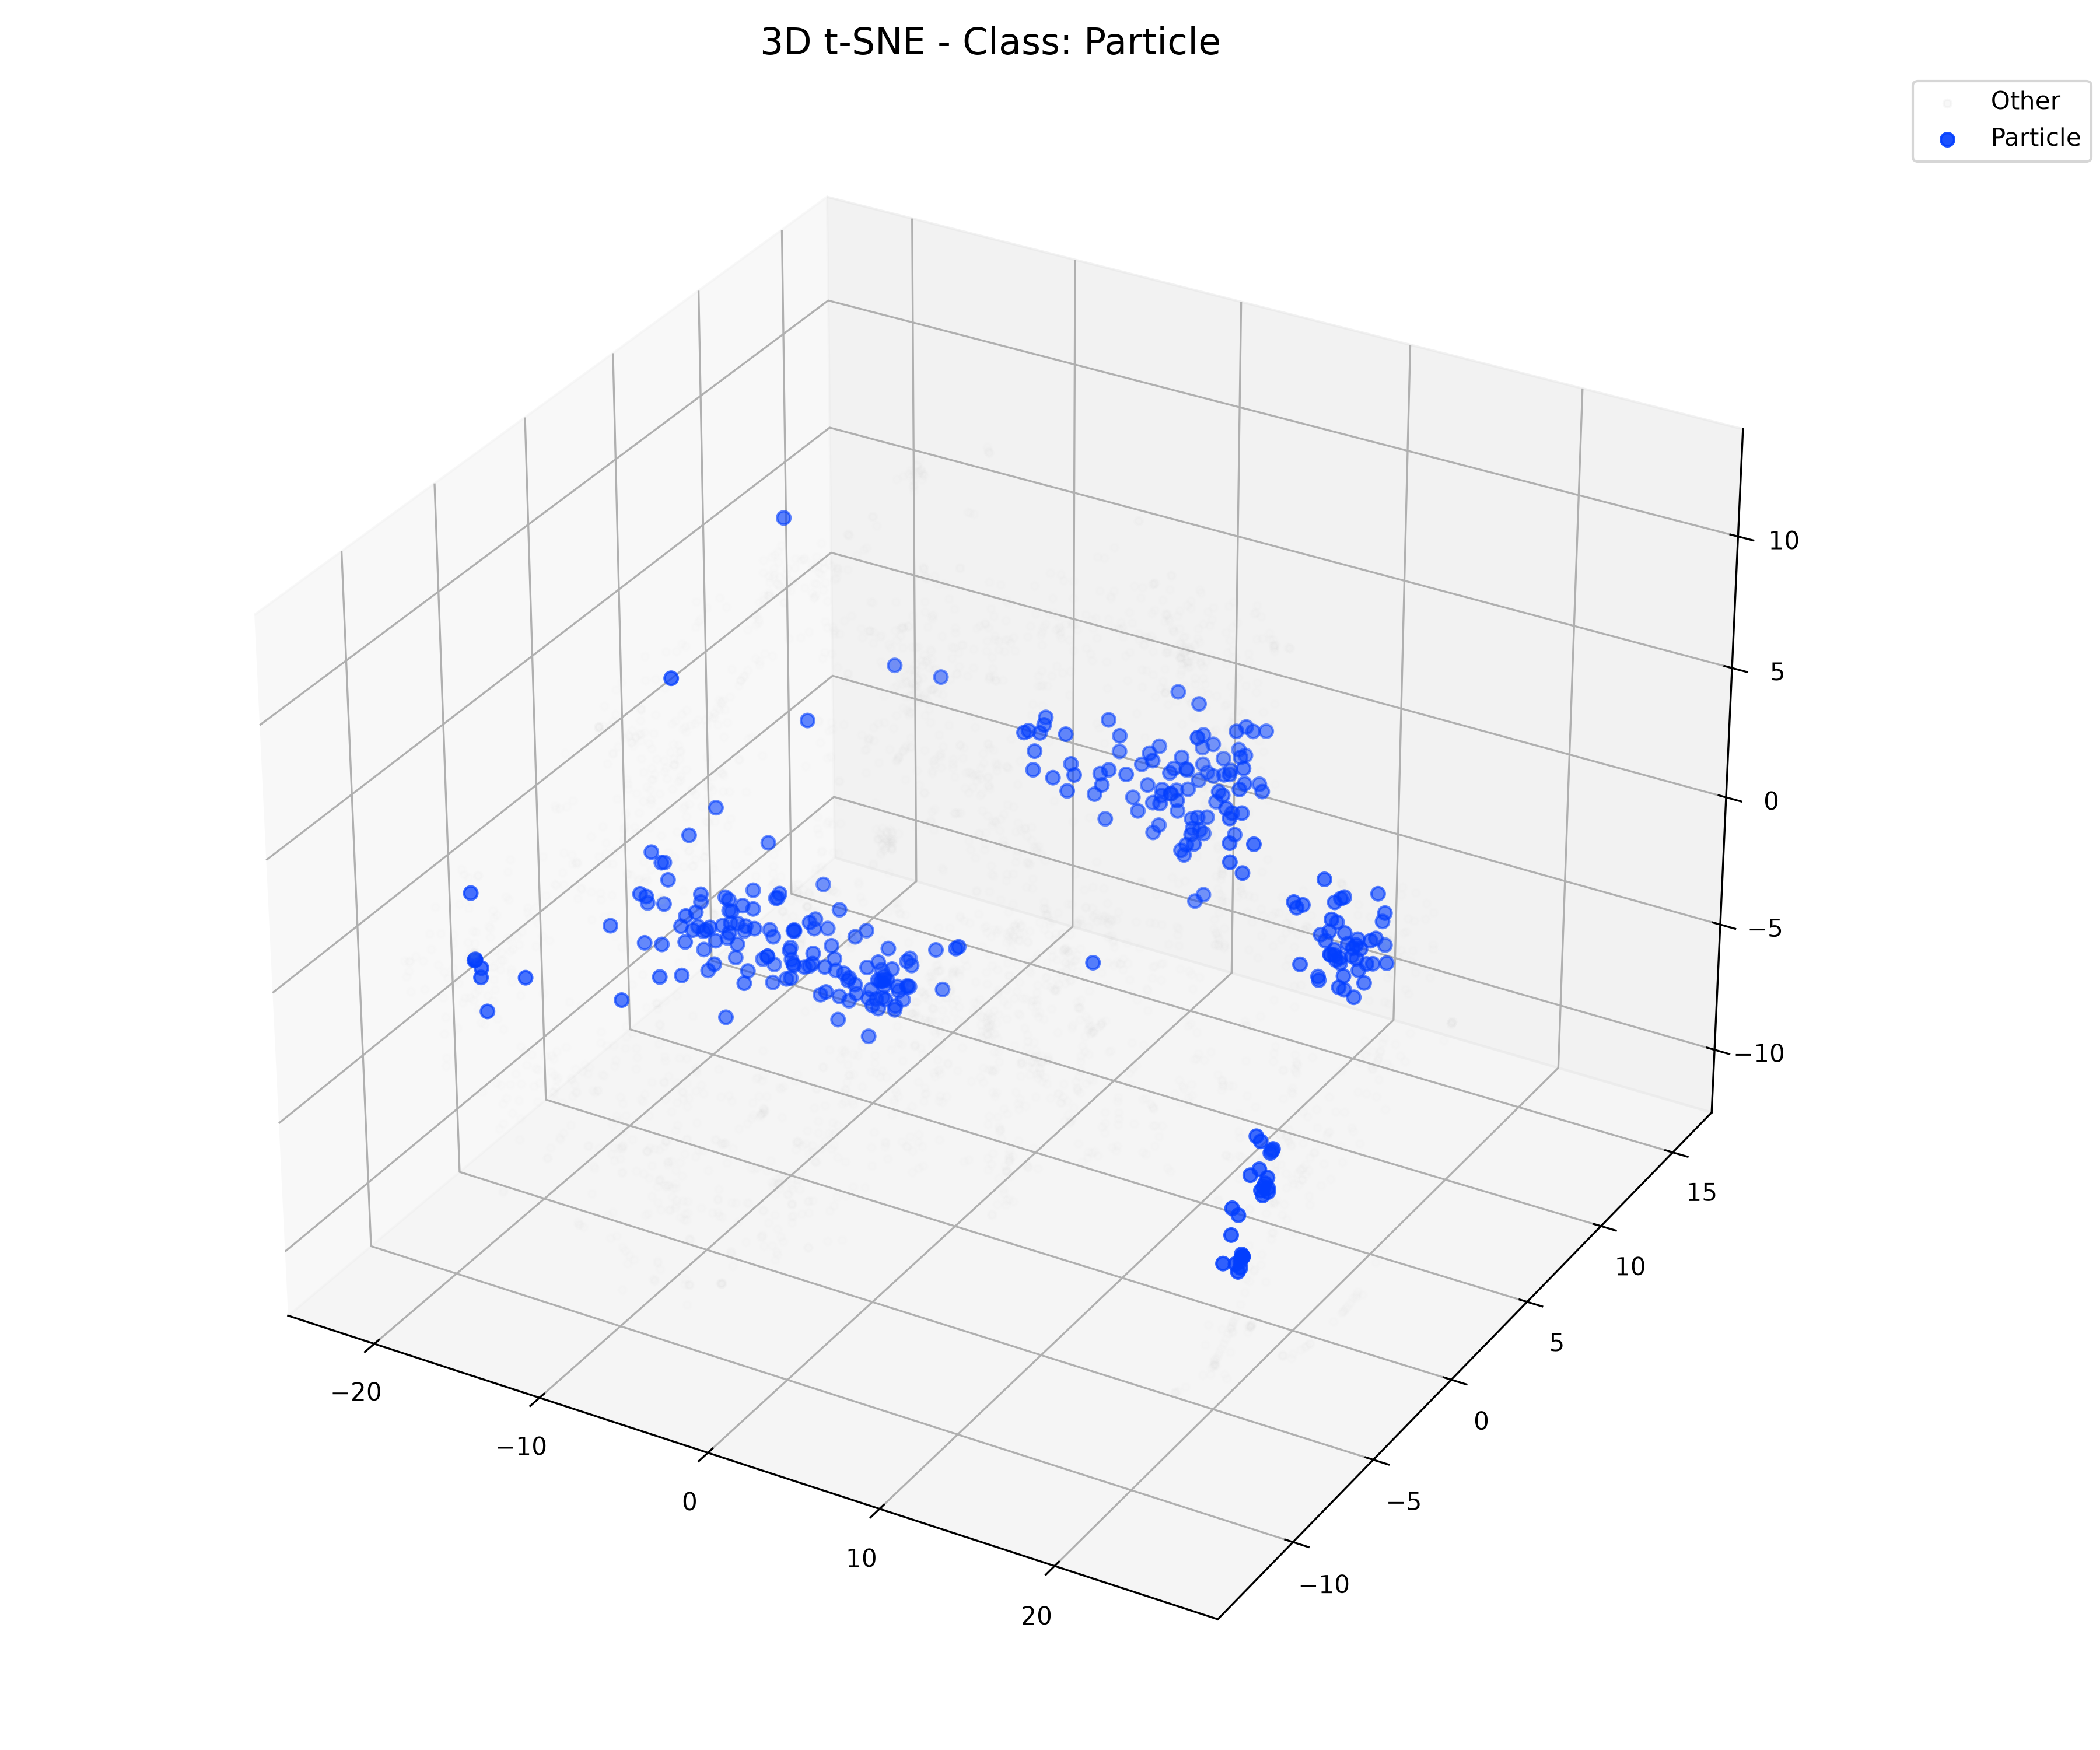
\includegraphics[width=\textwidth]{../Results/tsne_plots/data_by_type/split_3d_Particle.png}
        \caption{3D t-SNE: Particle}
    \end{subfigure}
    \caption{Highlighted distribution of Particle discharges.}
\end{figure}

% Void
\begin{figure}[H]
    \centering
    \begin{subfigure}[b]{0.45\textwidth}
        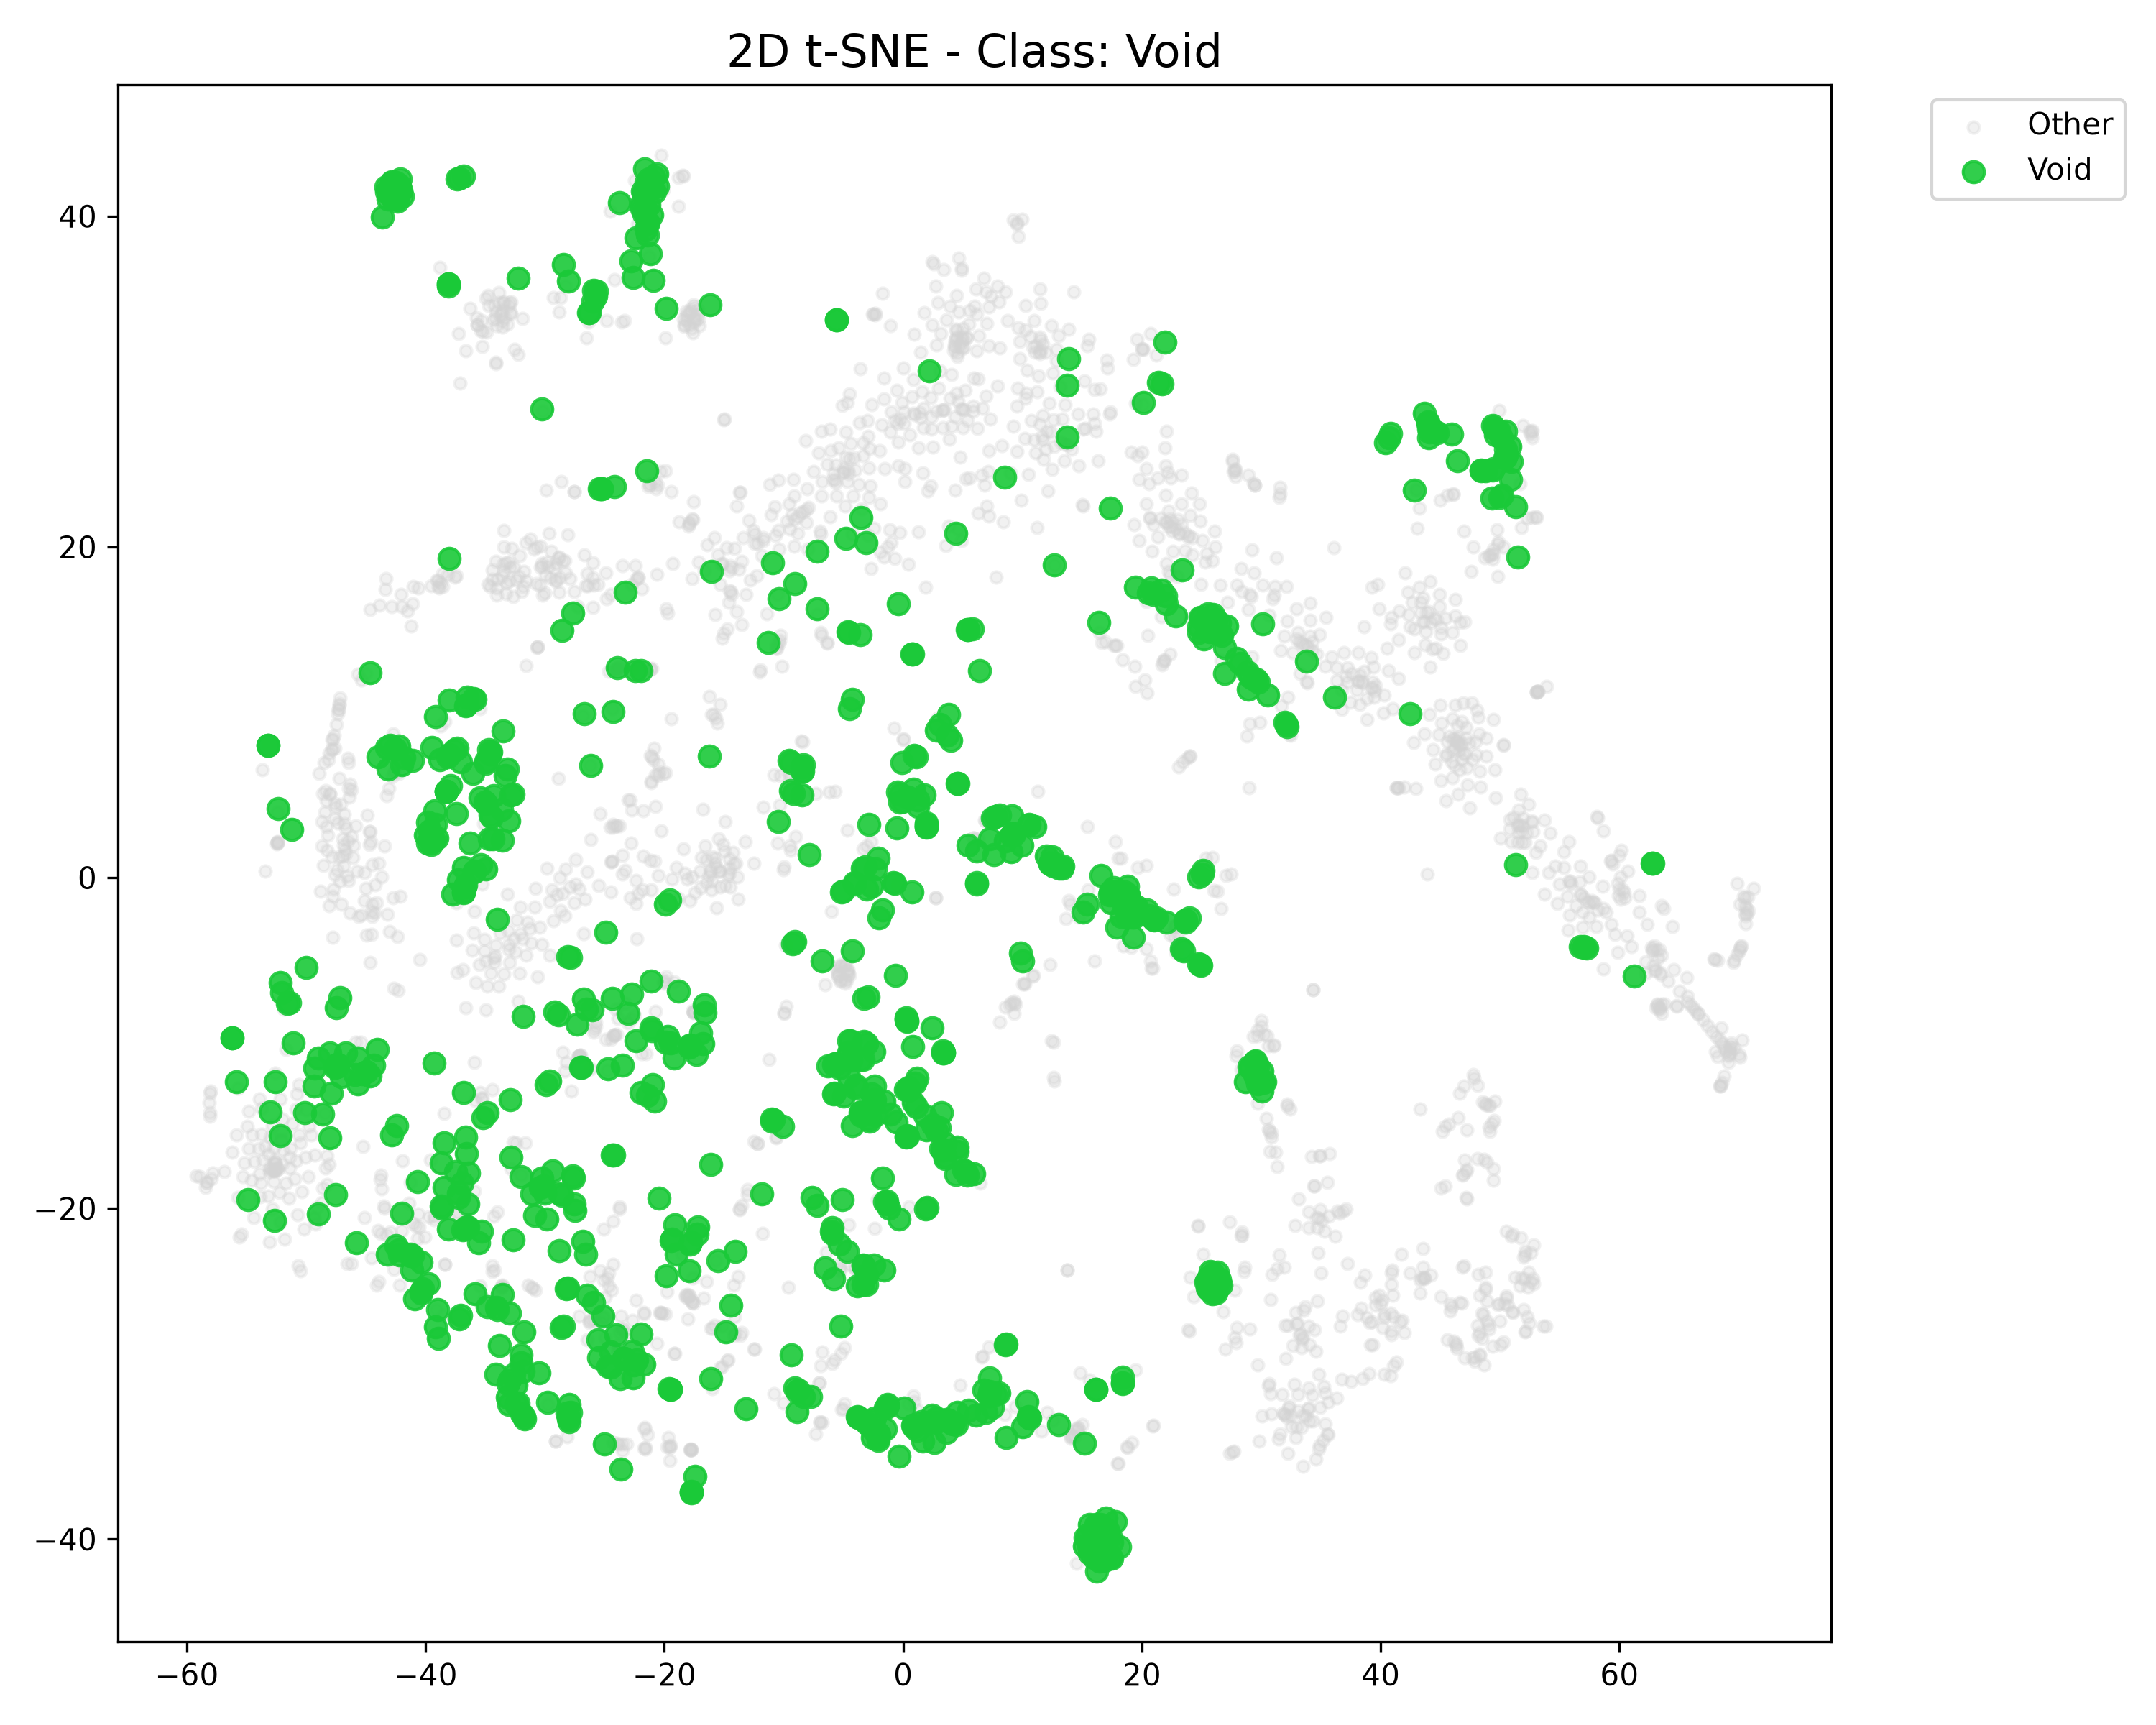
\includegraphics[width=\textwidth]{../Results/tsne_plots/data_by_type/split_2d_Void.png}
        \caption{2D t-SNE: Void}
    \end{subfigure}
    \hfill
    \begin{subfigure}[b]{0.45\textwidth}
        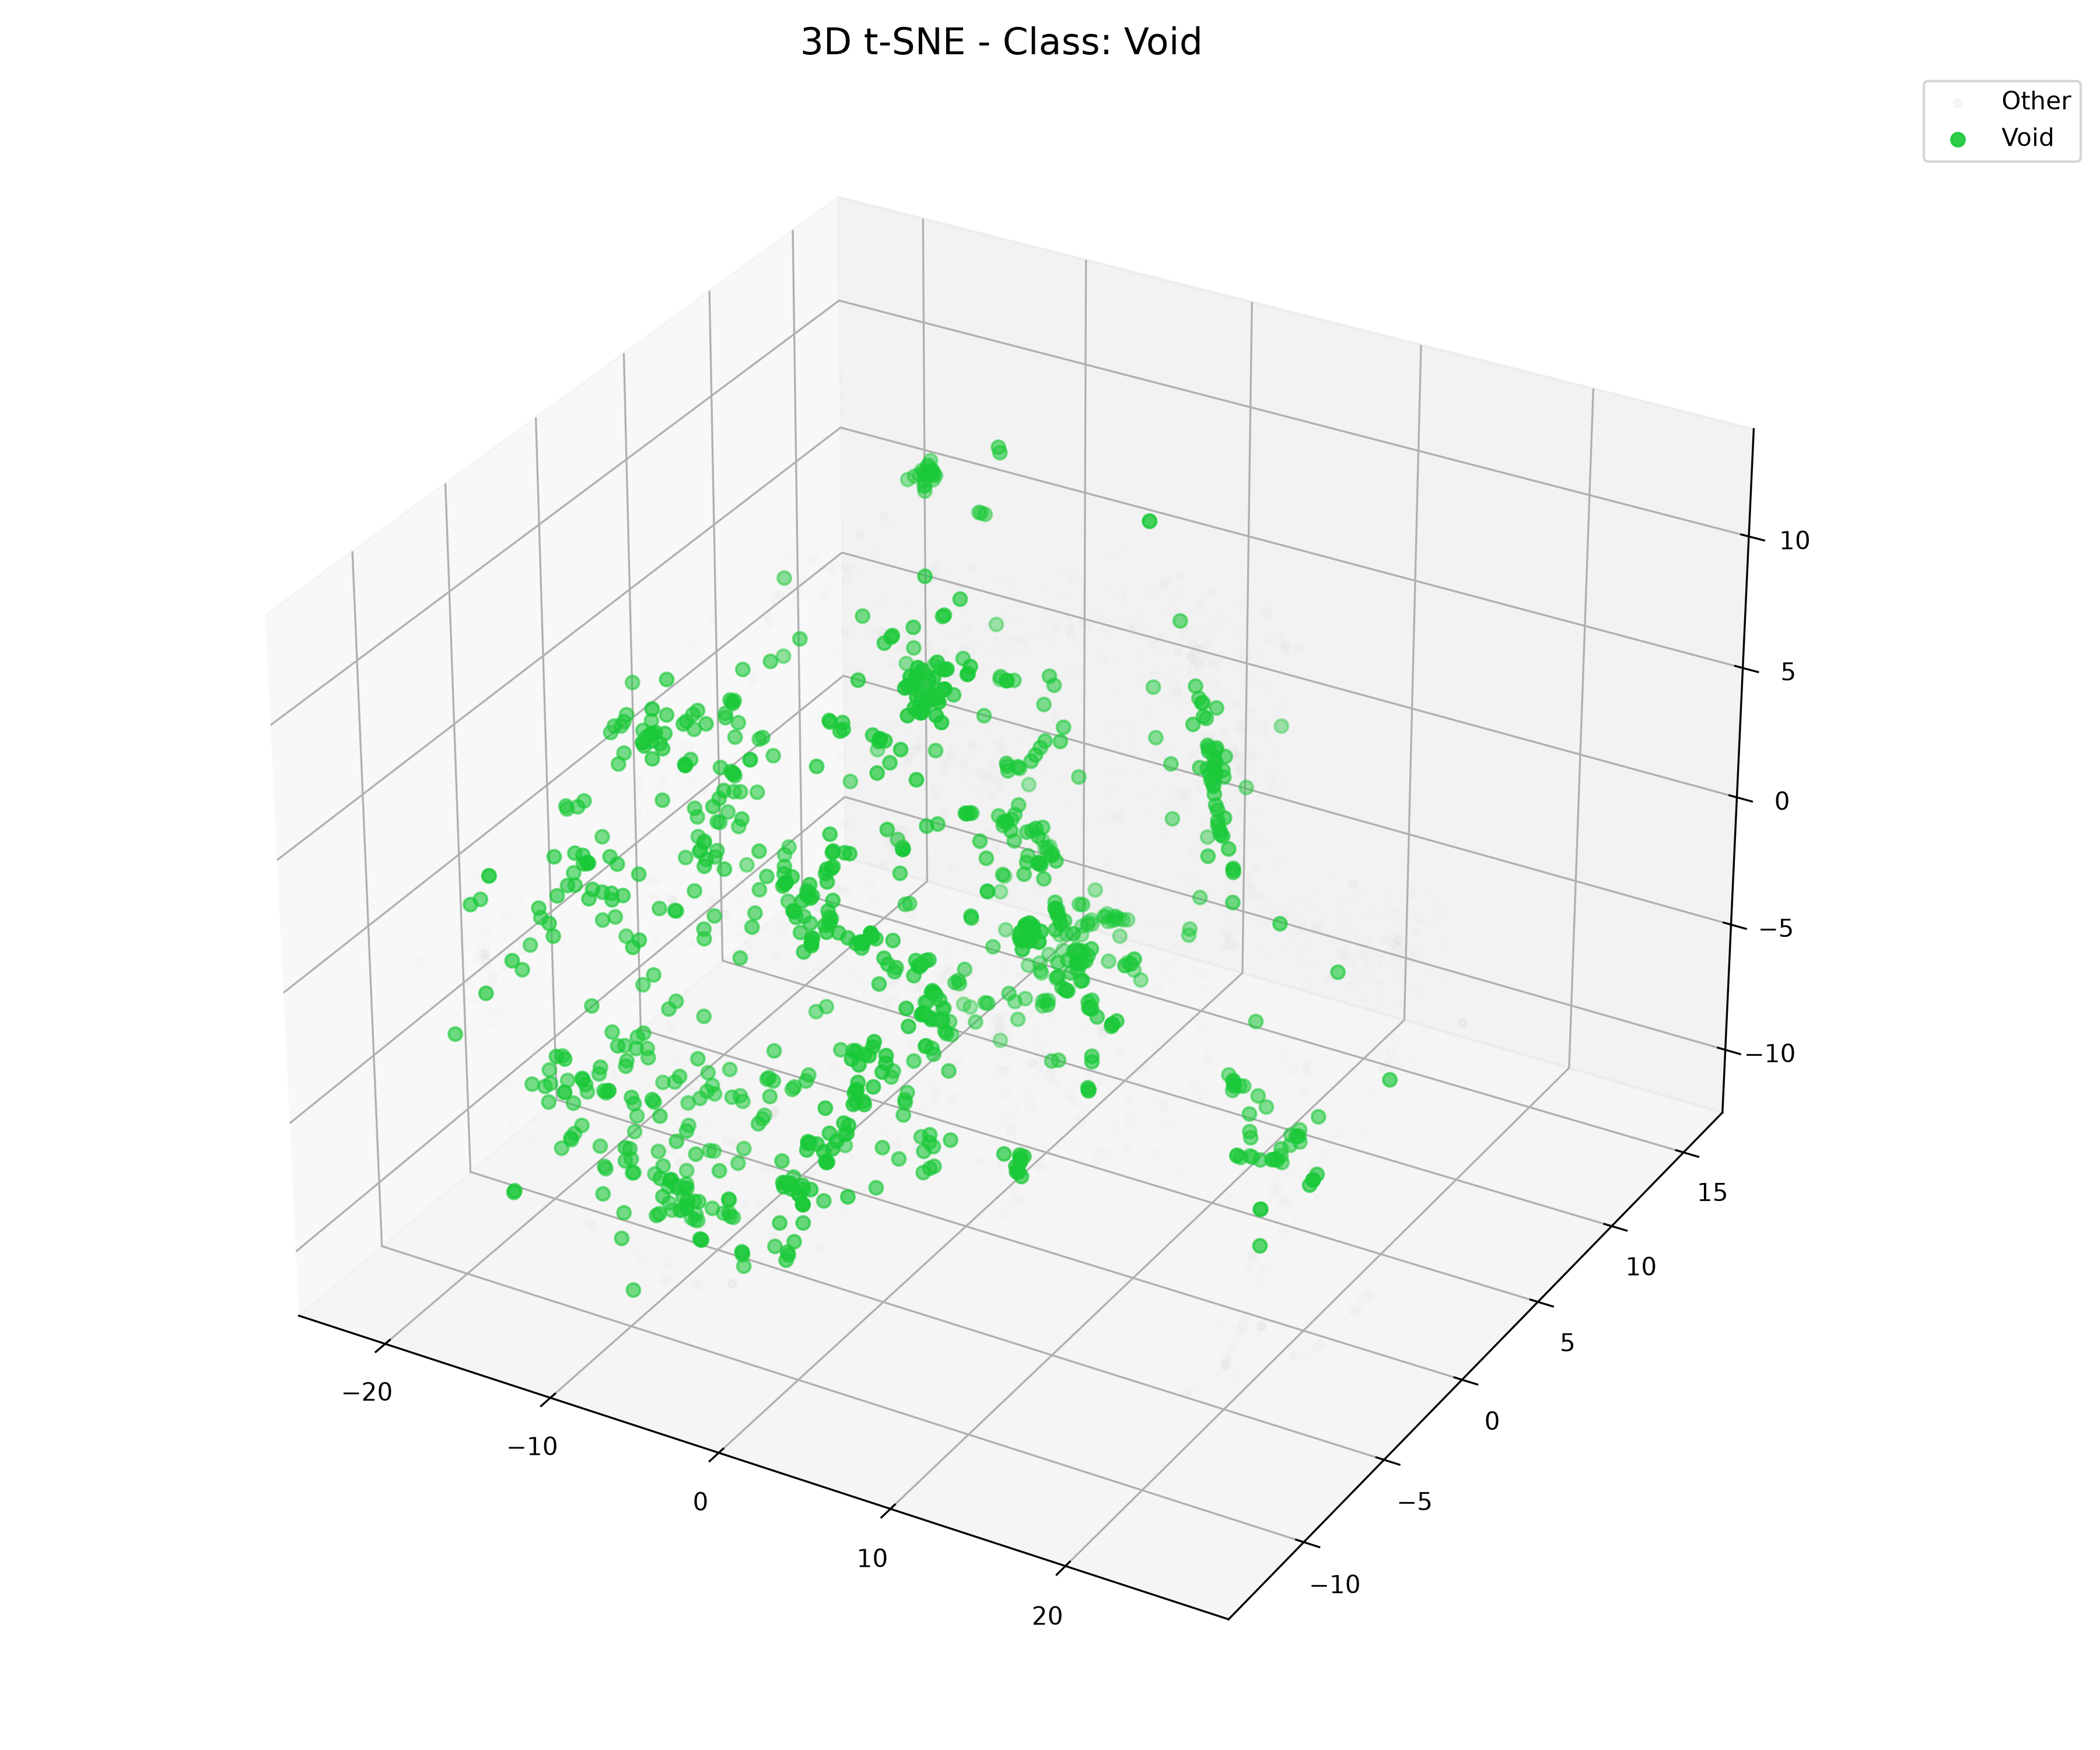
\includegraphics[width=\textwidth]{../Results/tsne_plots/data_by_type/split_3d_Void.png}
        \caption{3D t-SNE: Void}
    \end{subfigure}
    \caption{Highlighted distribution of Void discharges.}
\end{figure}

% Noise
\begin{figure}[H]
    \centering
    \begin{subfigure}[b]{0.45\textwidth}
        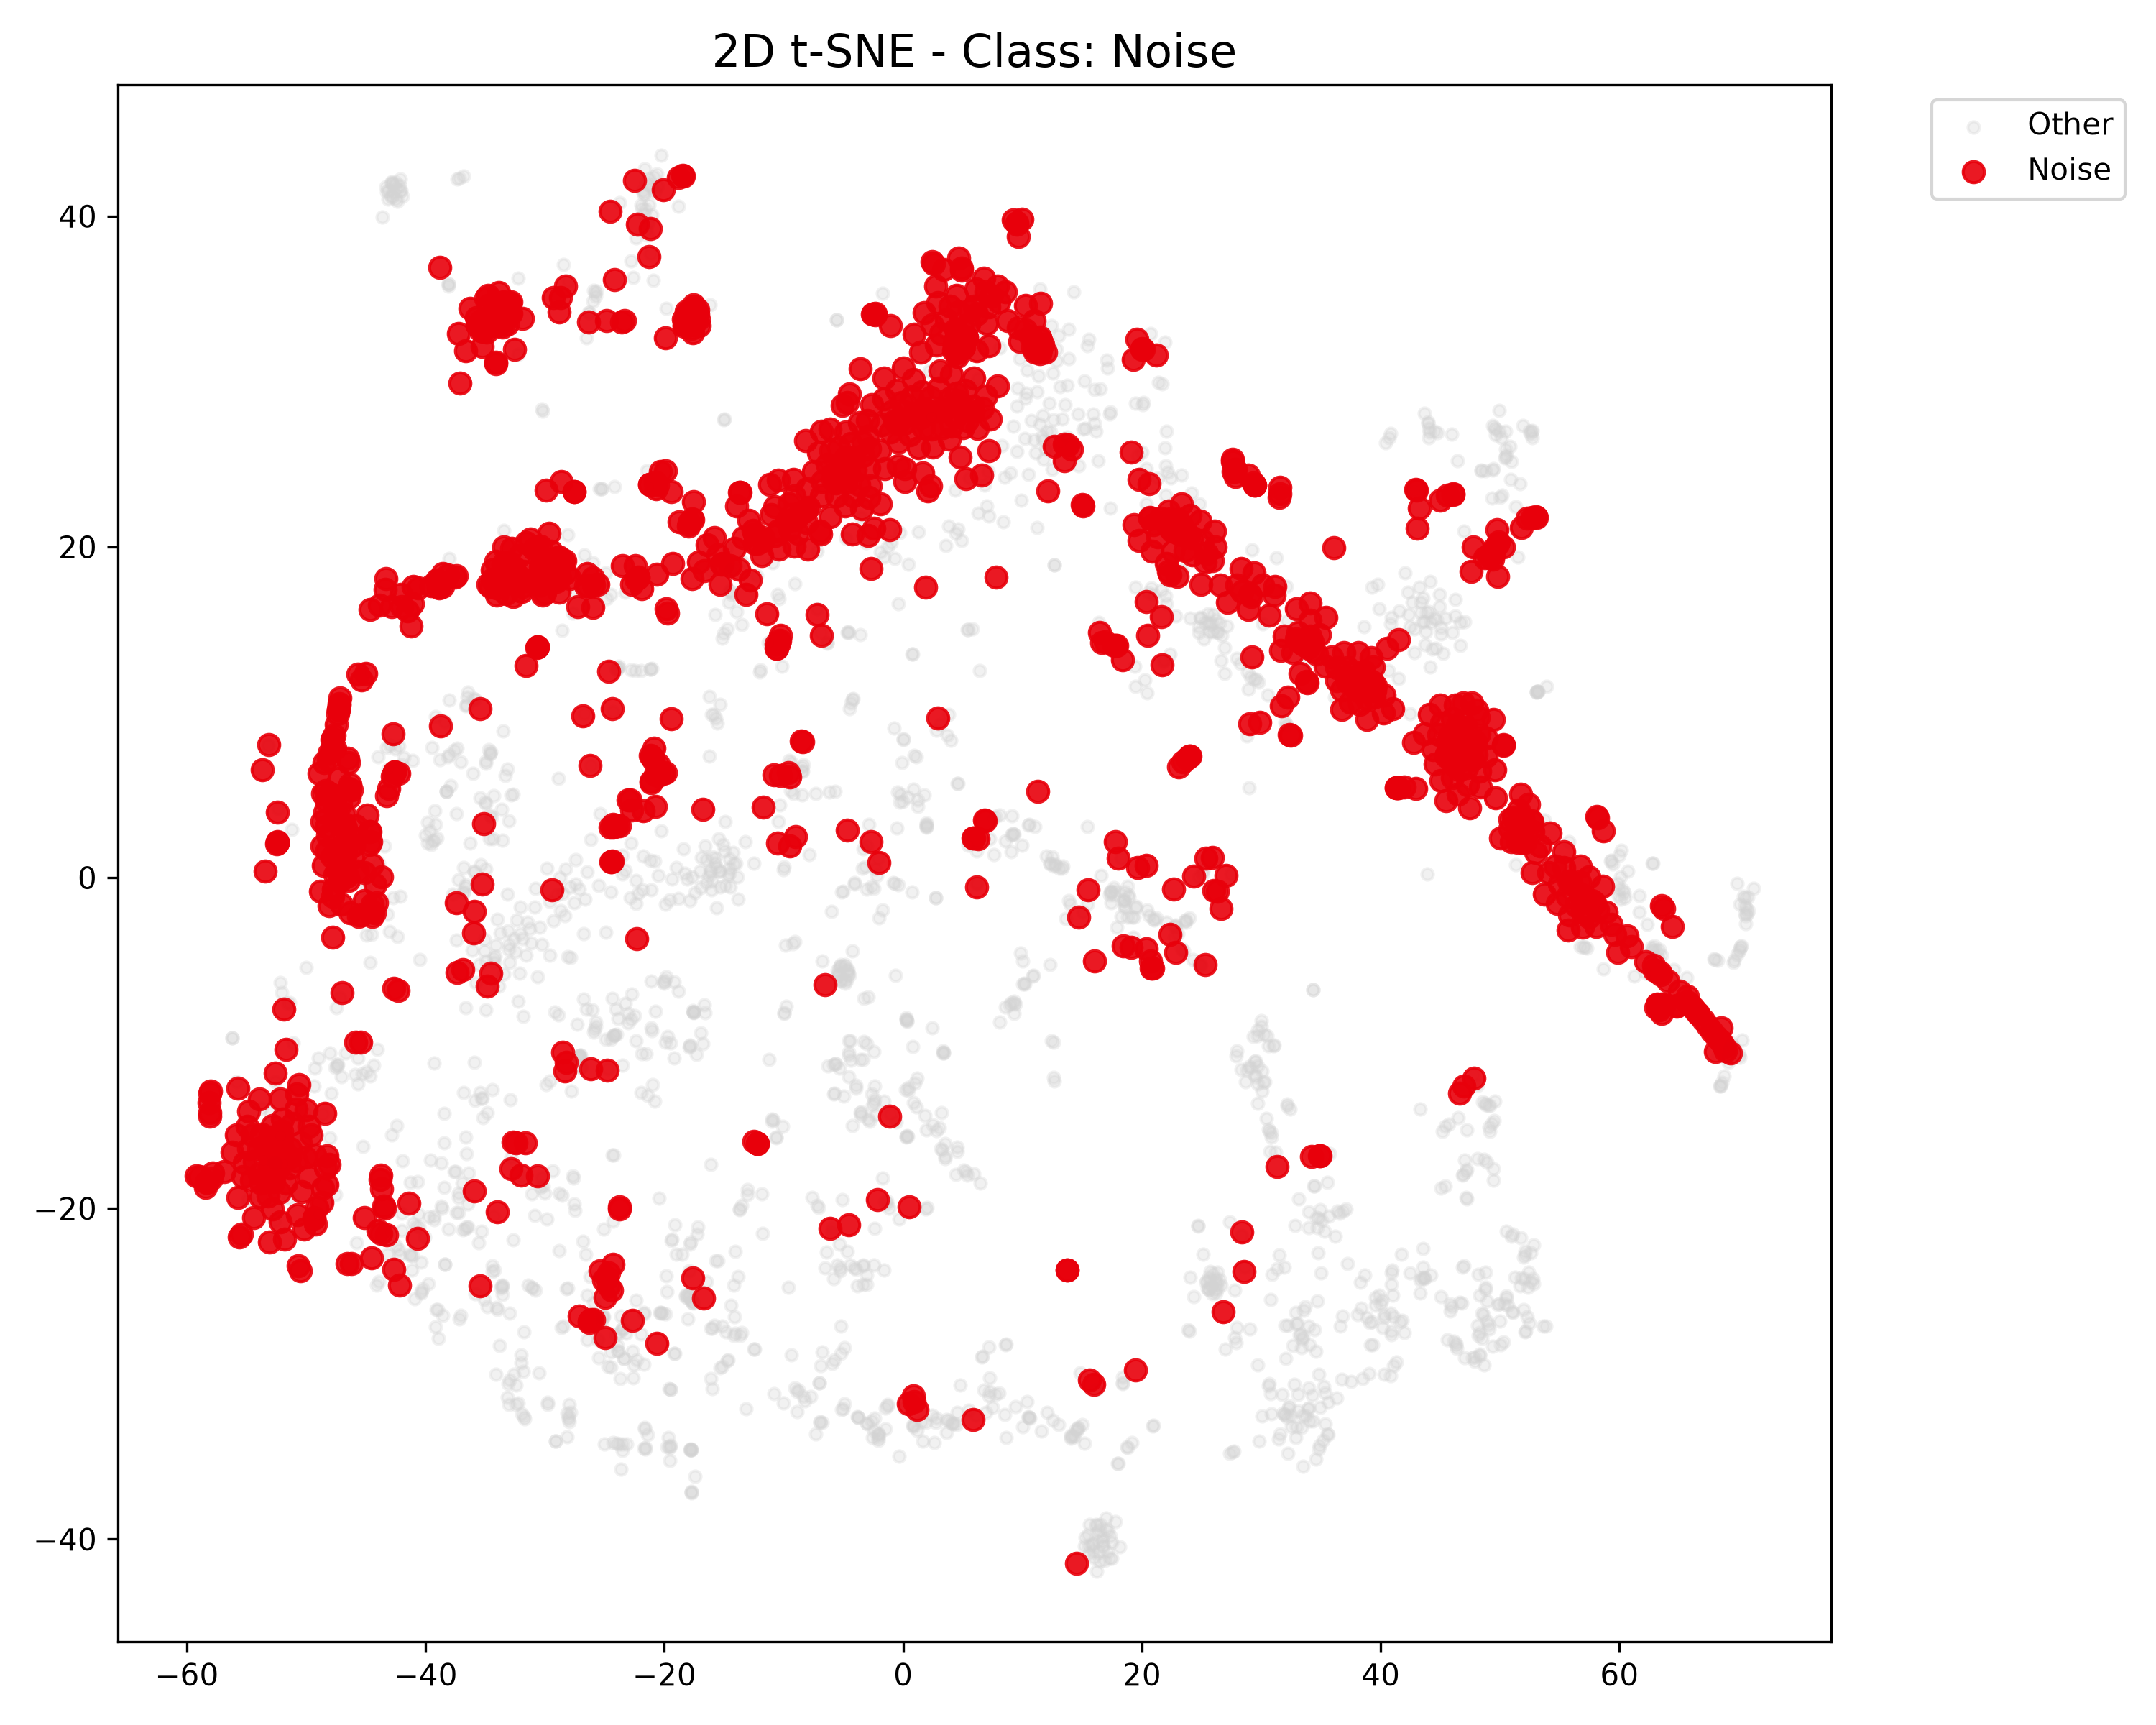
\includegraphics[width=\textwidth]{../Results/tsne_plots/data_by_type/split_2d_Noise.png}
        \caption{2D t-SNE: Noise}
    \end{subfigure}
    \hfill
    \begin{subfigure}[b]{0.45\textwidth}
        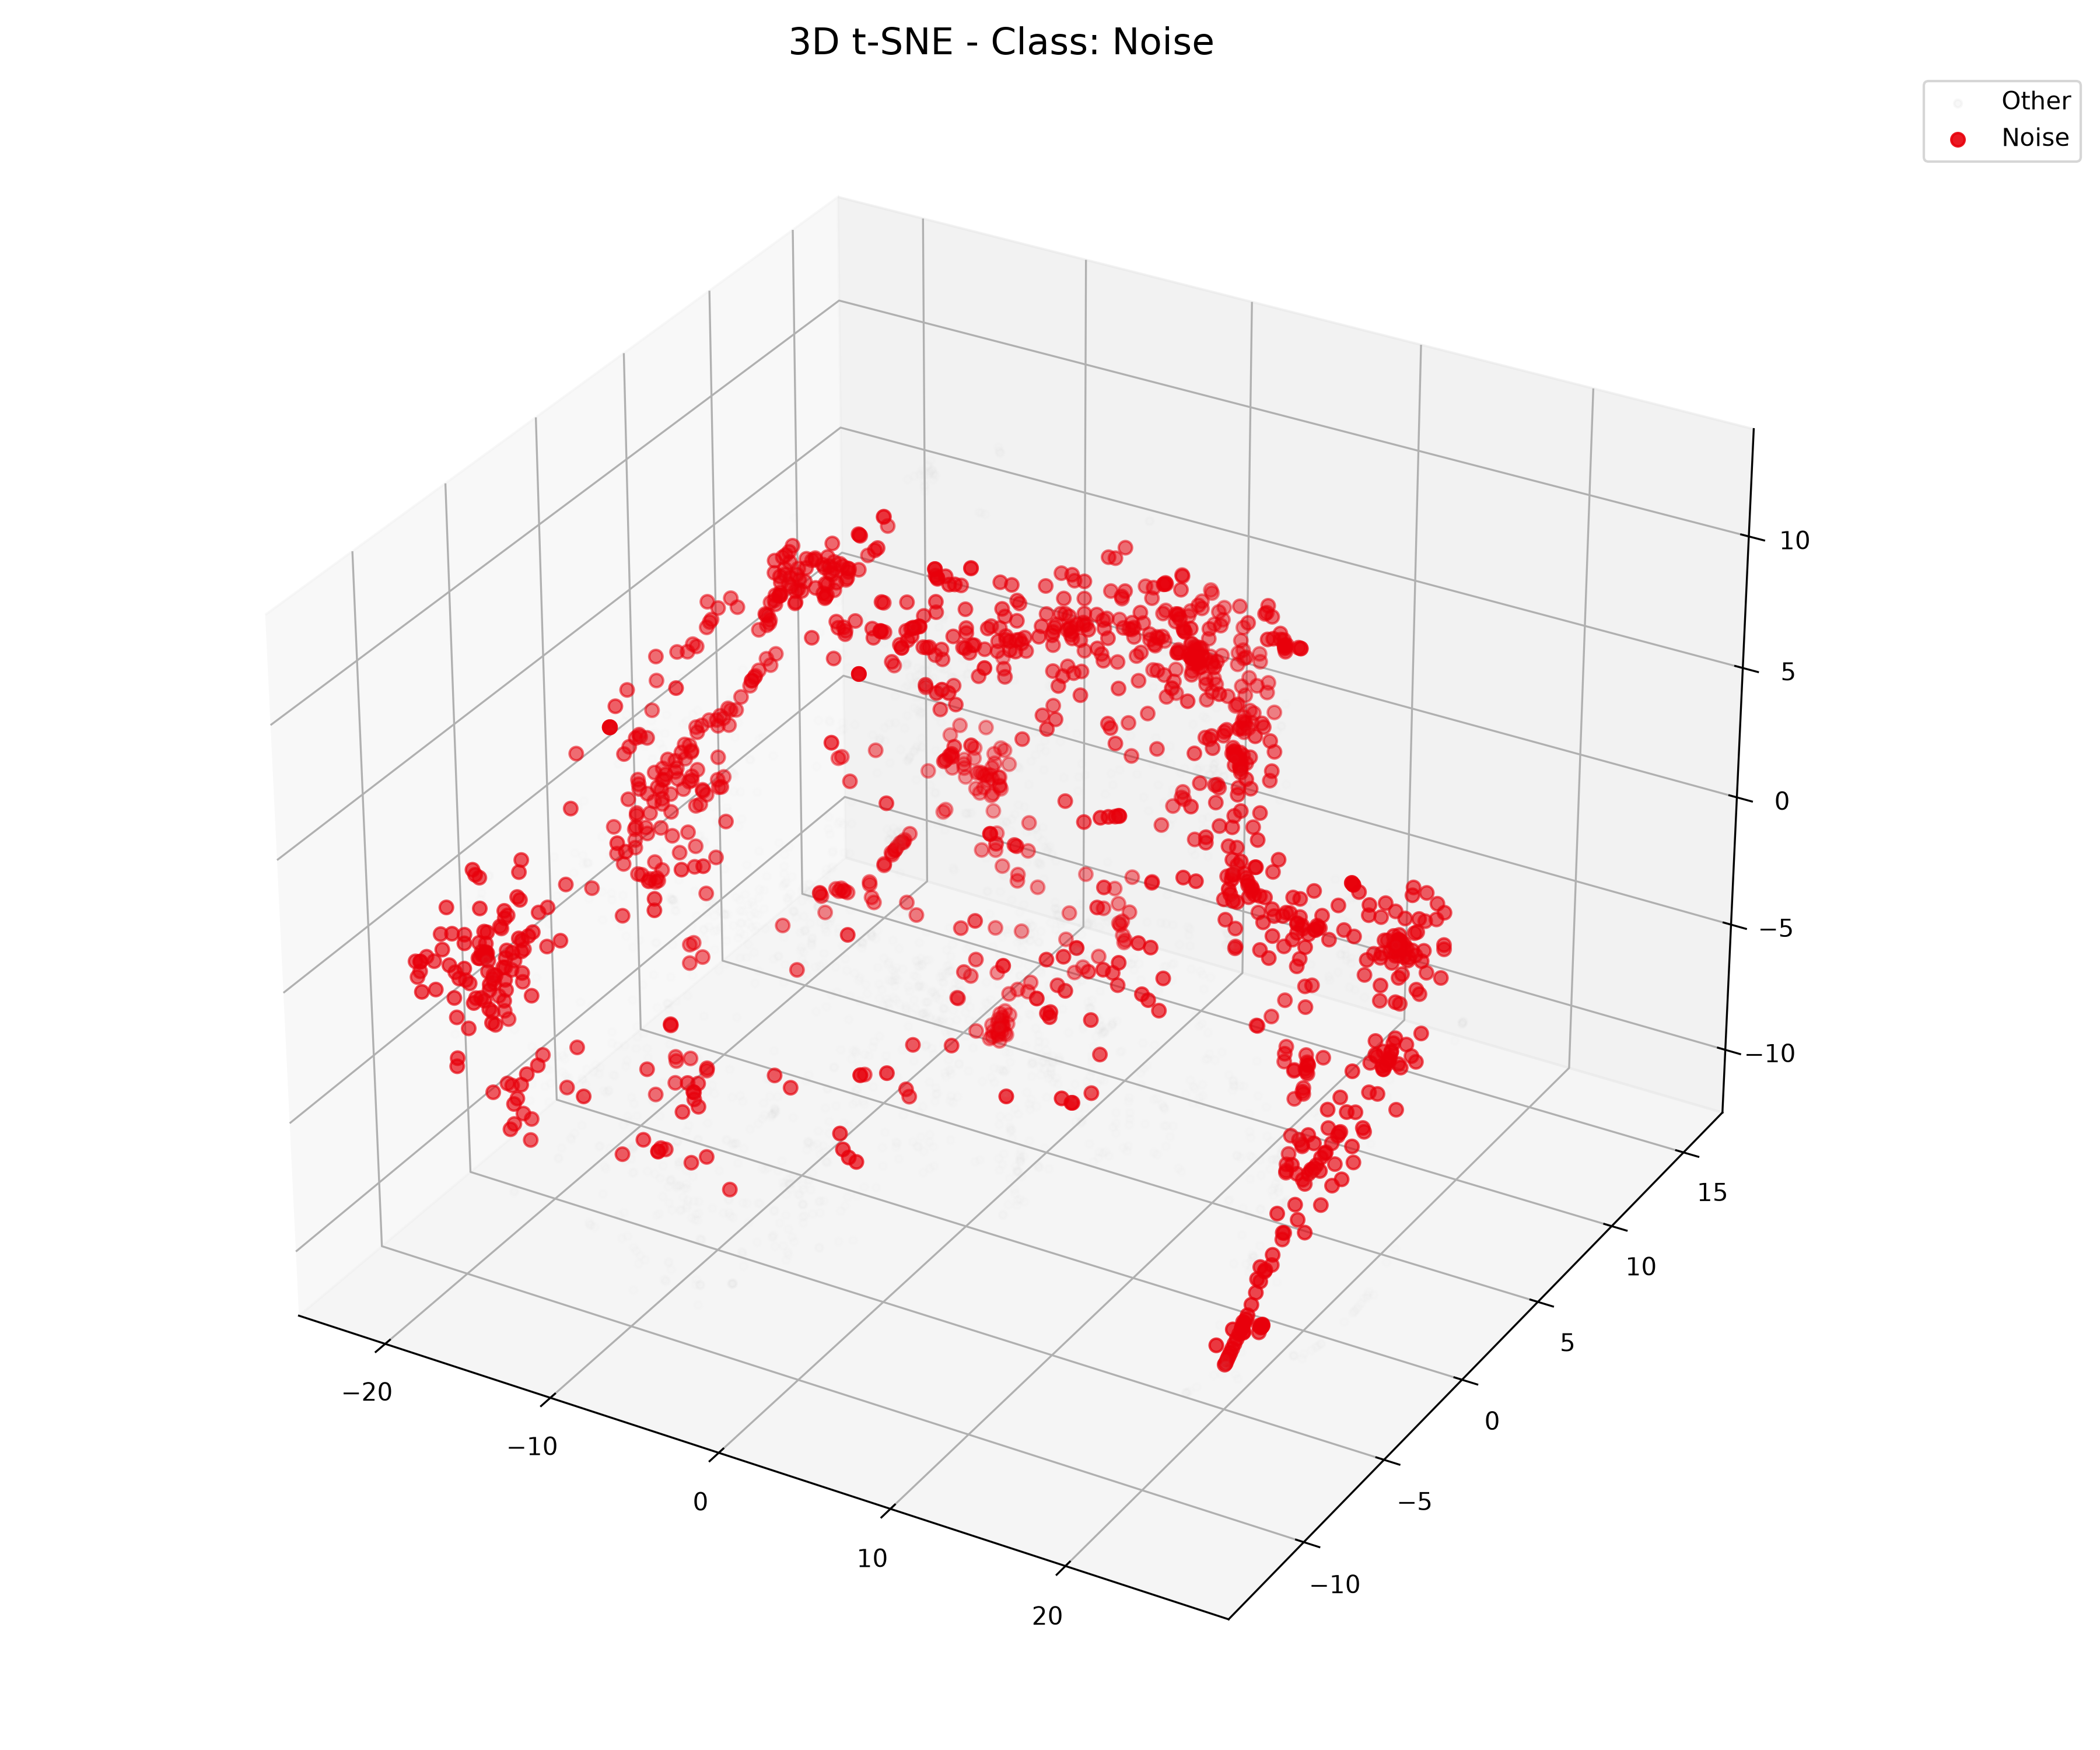
\includegraphics[width=\textwidth]{../Results/tsne_plots/data_by_type/split_3d_Noise.png}
        \caption{3D t-SNE: Noise}
    \end{subfigure}
    \caption{Highlighted distribution of Noise samples.}
\end{figure}

\clearpage

\section{Visualizations: Data Organized by Date}
This section illustrates the dataset organized by collection date context. While the underlying data points remain consistent, mapping the exact PD labels back to the chronological distribution reveals the structure within the temporal field/lab collections.

\subsection{Global Clusters (Data by Date)}
\begin{figure}[H]
    \centering
    \begin{subfigure}[b]{0.45\textwidth}
        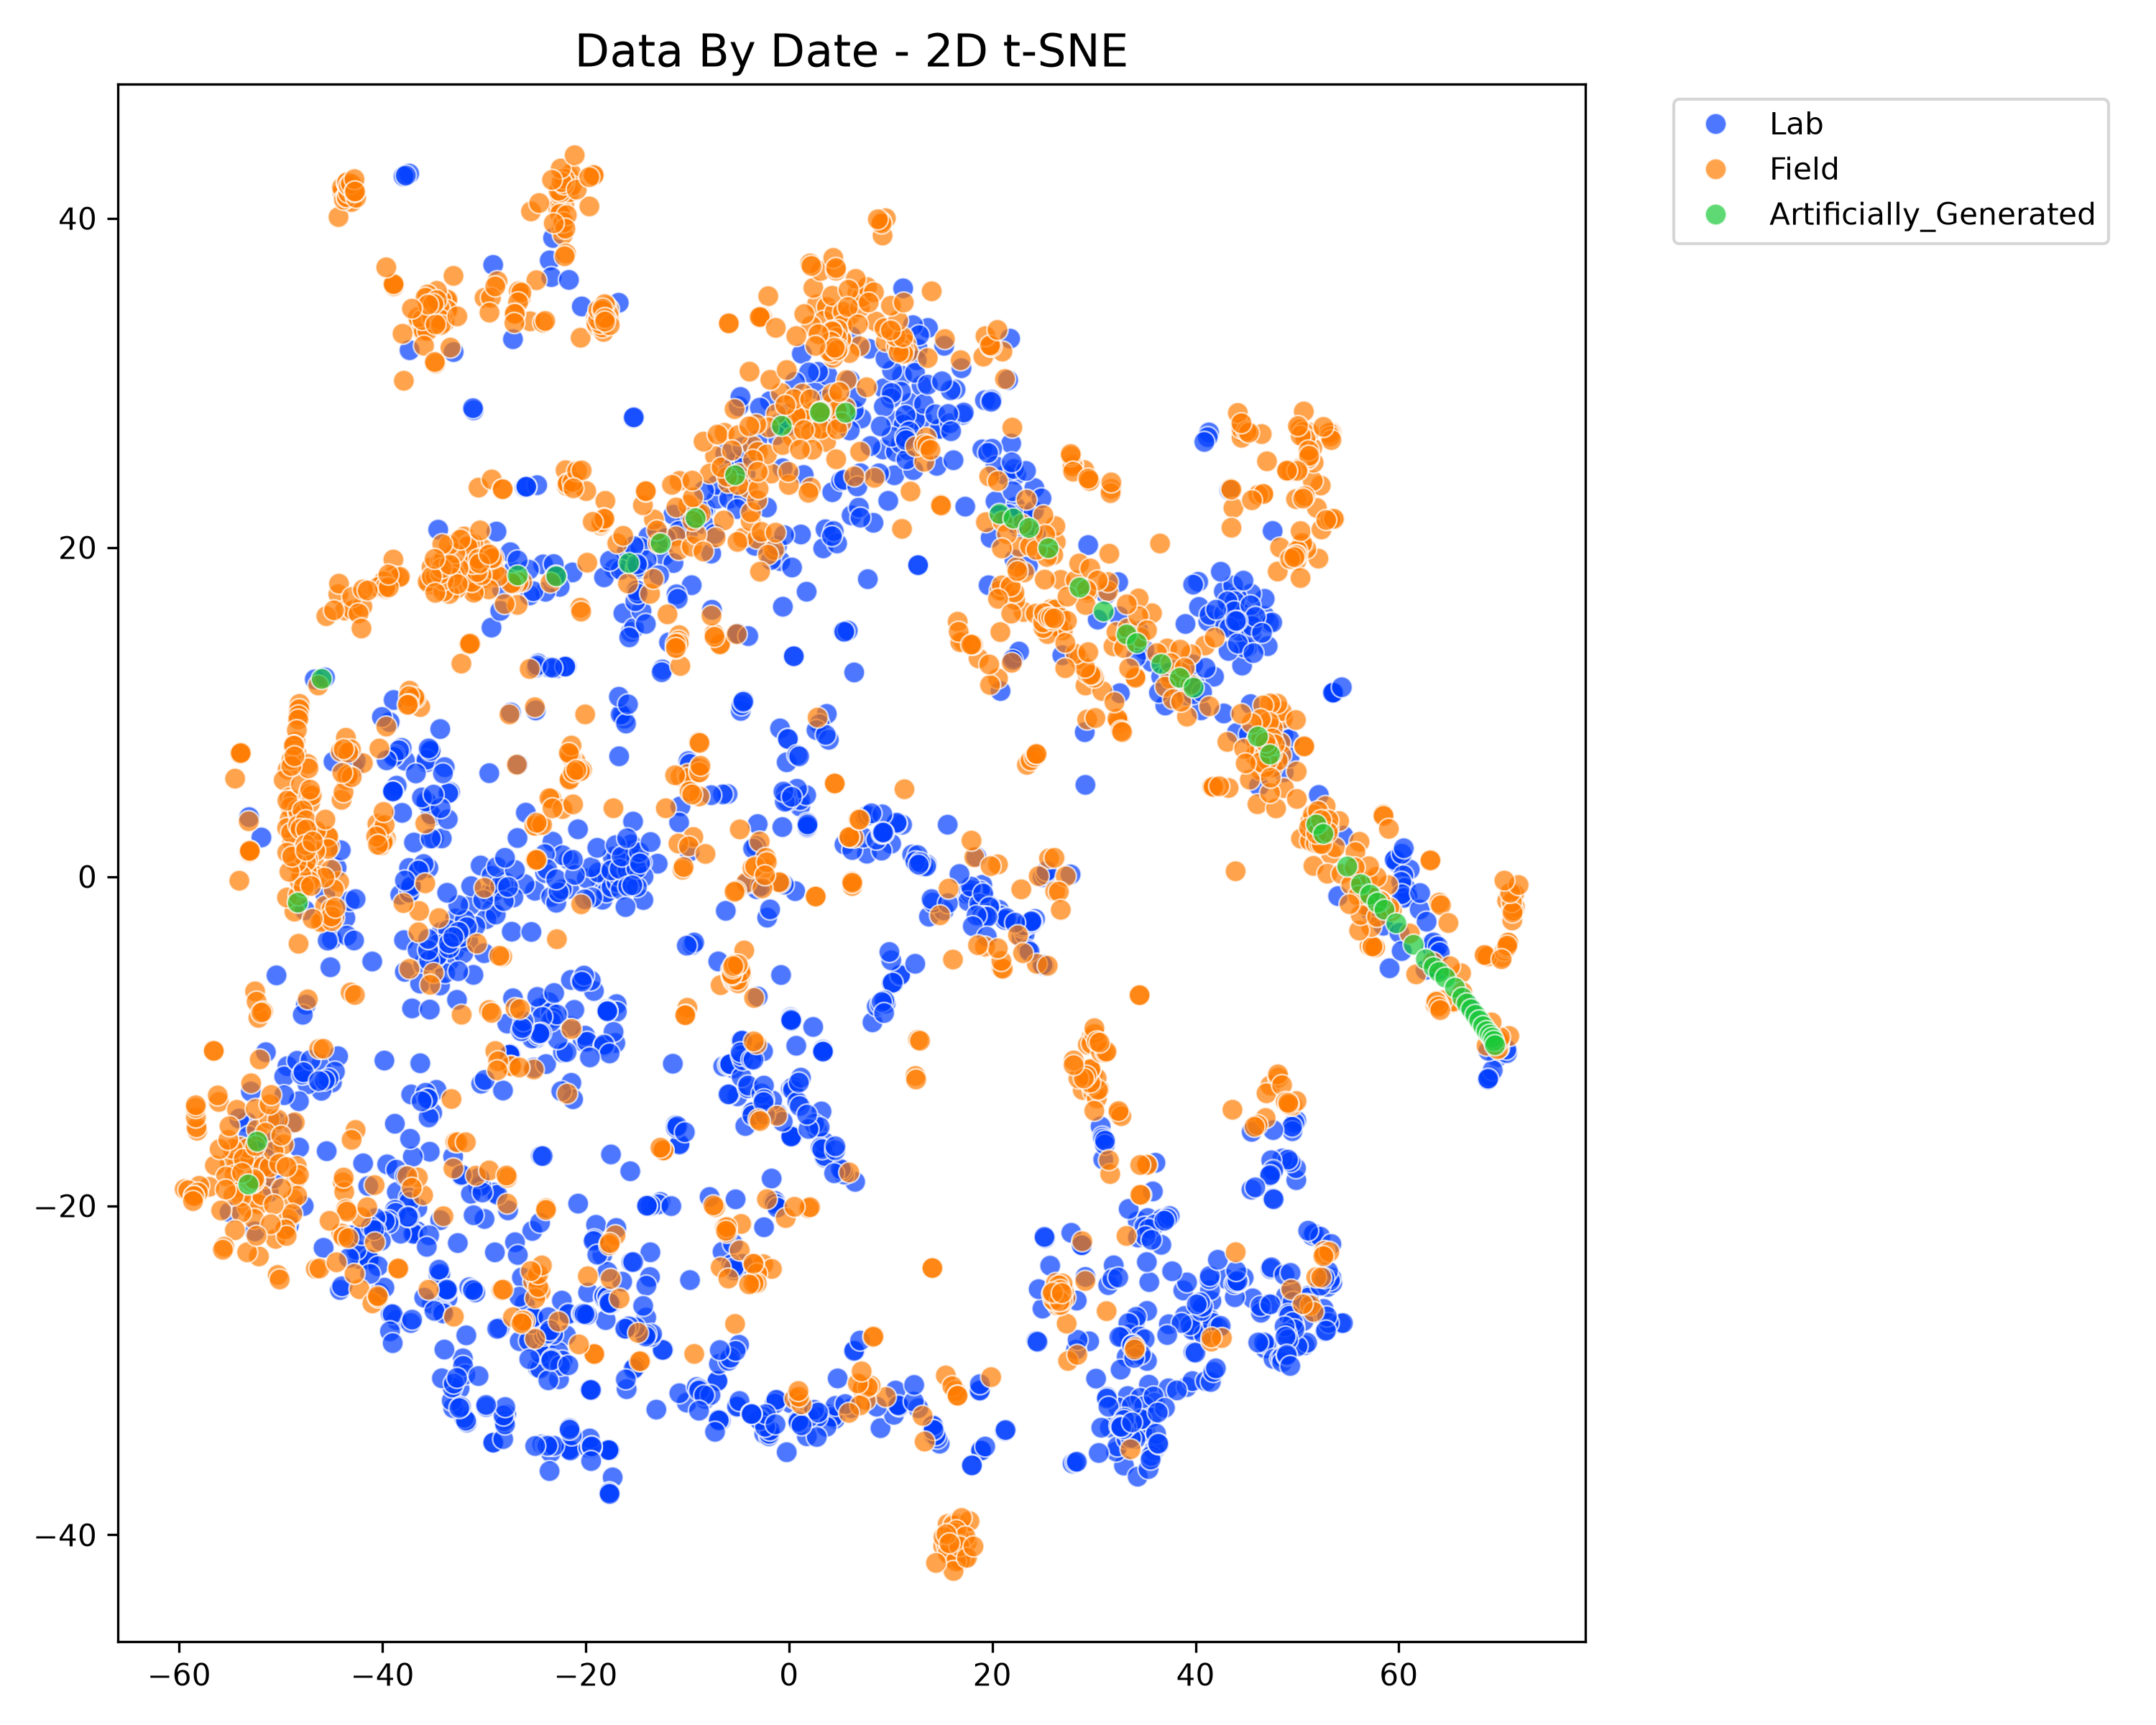
\includegraphics[width=\textwidth]{../Results/tsne_plots/data_by_date/2d_plot.png}
        \caption{Global 2D t-SNE}
    \end{subfigure}
    \hfill
    \begin{subfigure}[b]{0.45\textwidth}
        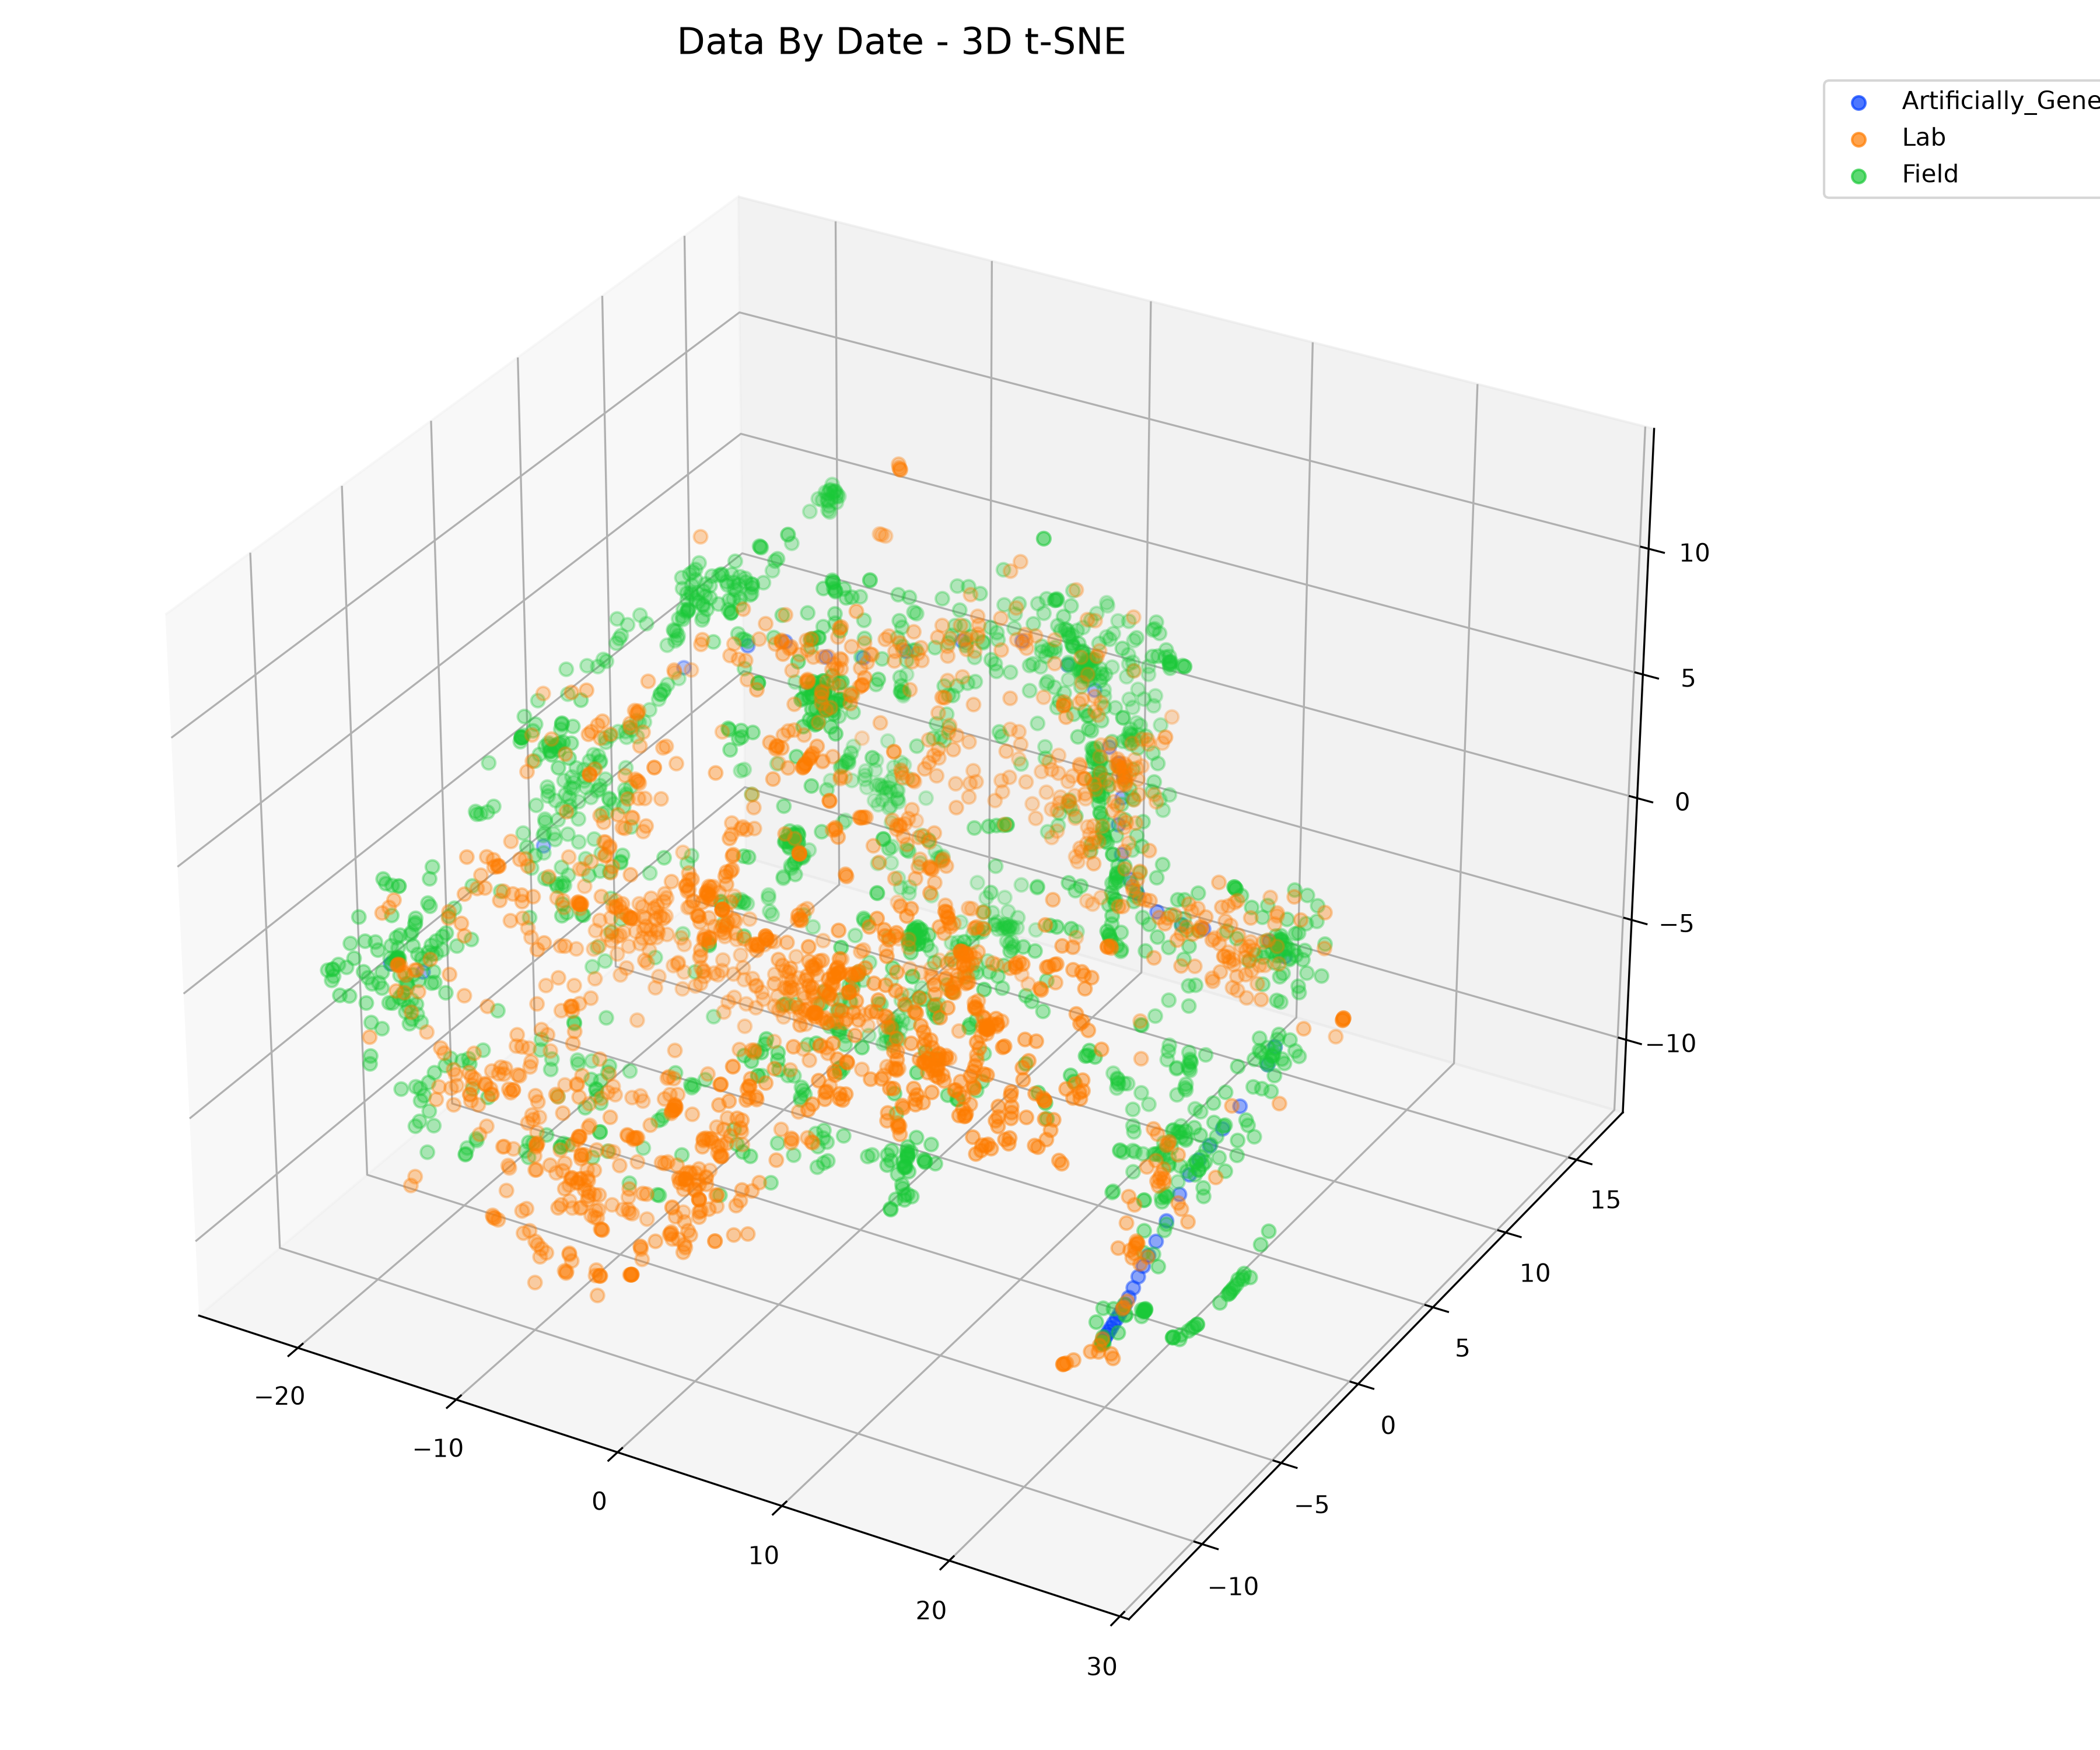
\includegraphics[width=\textwidth]{../Results/tsne_plots/data_by_date/3d_plot.png}
        \caption{Global 3D t-SNE}
    \end{subfigure}
    \caption{Global t-SNE projections for all collections in \texttt{data\_by\_date}.}
\end{figure}

\subsection{Class-Specific Projections (Data by Date)}

% Corona
\begin{figure}[H]
    \centering
    \begin{subfigure}[b]{0.45\textwidth}
        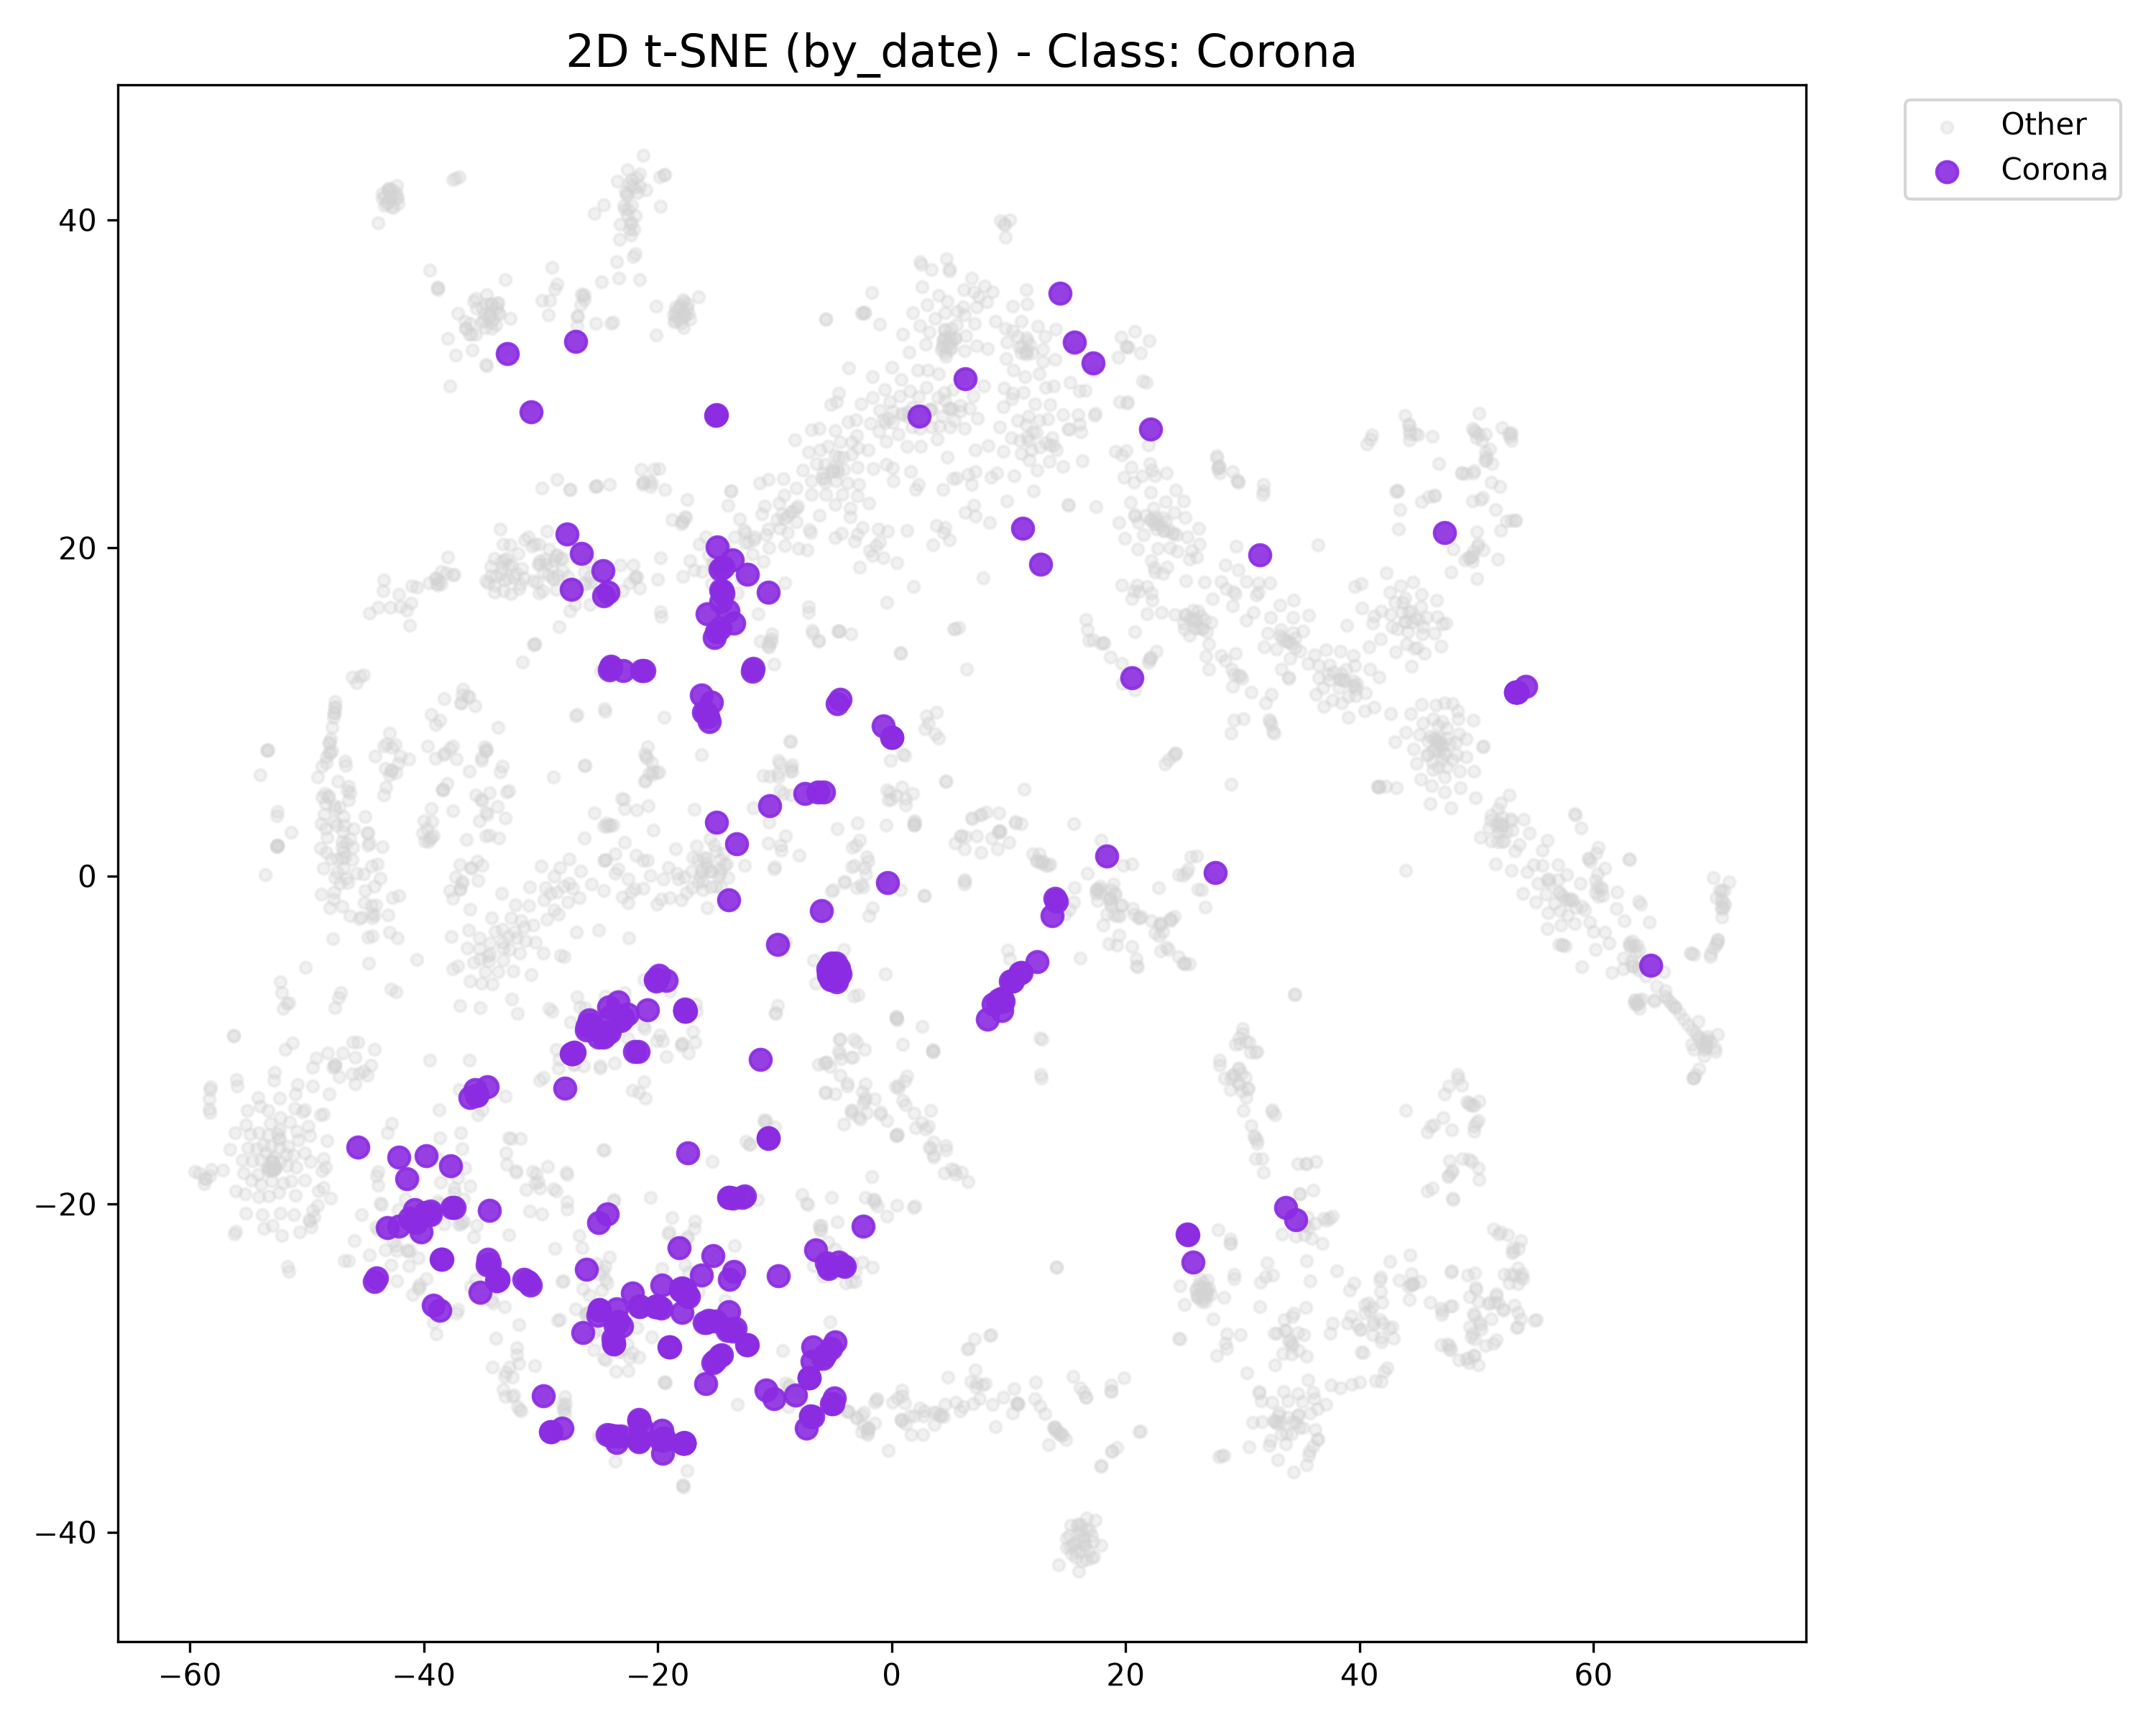
\includegraphics[width=\textwidth]{../Results/tsne_plots/data_by_date/split_2d_Corona.png}
        \caption{2D t-SNE: Corona}
    \end{subfigure}
    \hfill
    \begin{subfigure}[b]{0.45\textwidth}
        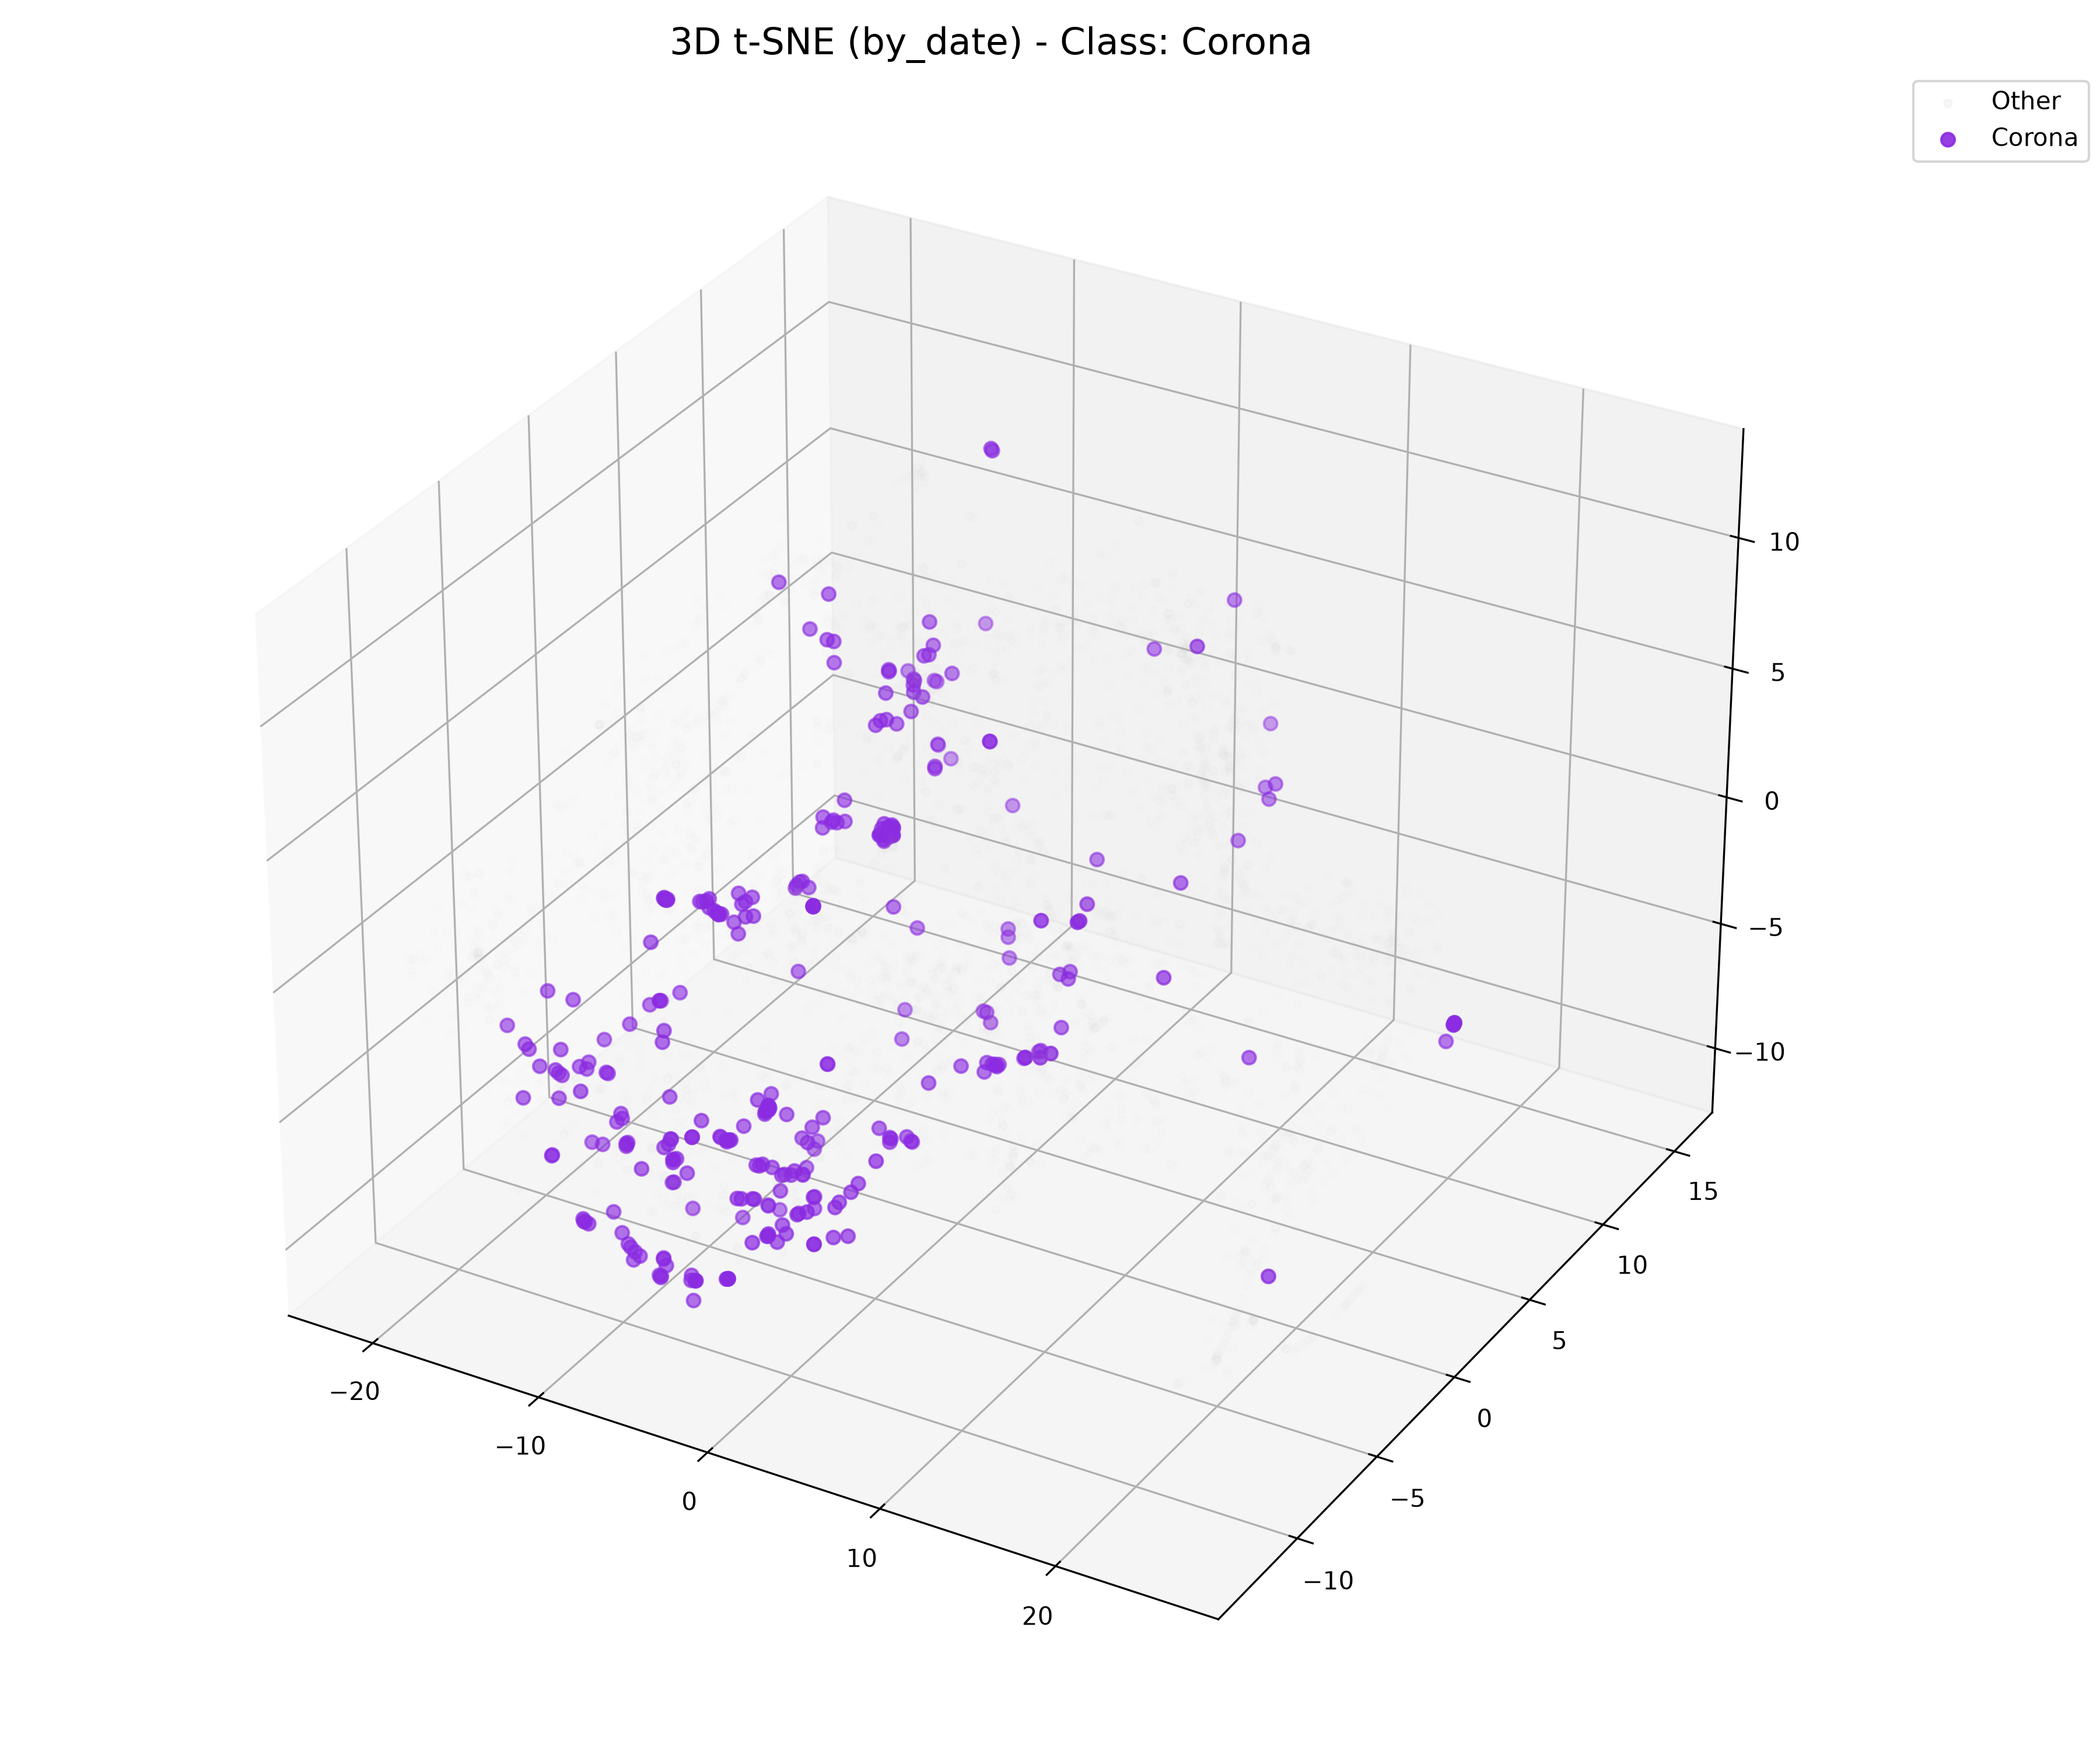
\includegraphics[width=\textwidth]{../Results/tsne_plots/data_by_date/split_3d_Corona.png}
        \caption{3D t-SNE: Corona}
    \end{subfigure}
    \caption{Highlighted distribution of Corona discharges within dated collections.}
\end{figure}

% Floating
\begin{figure}[H]
    \centering
    \begin{subfigure}[b]{0.45\textwidth}
        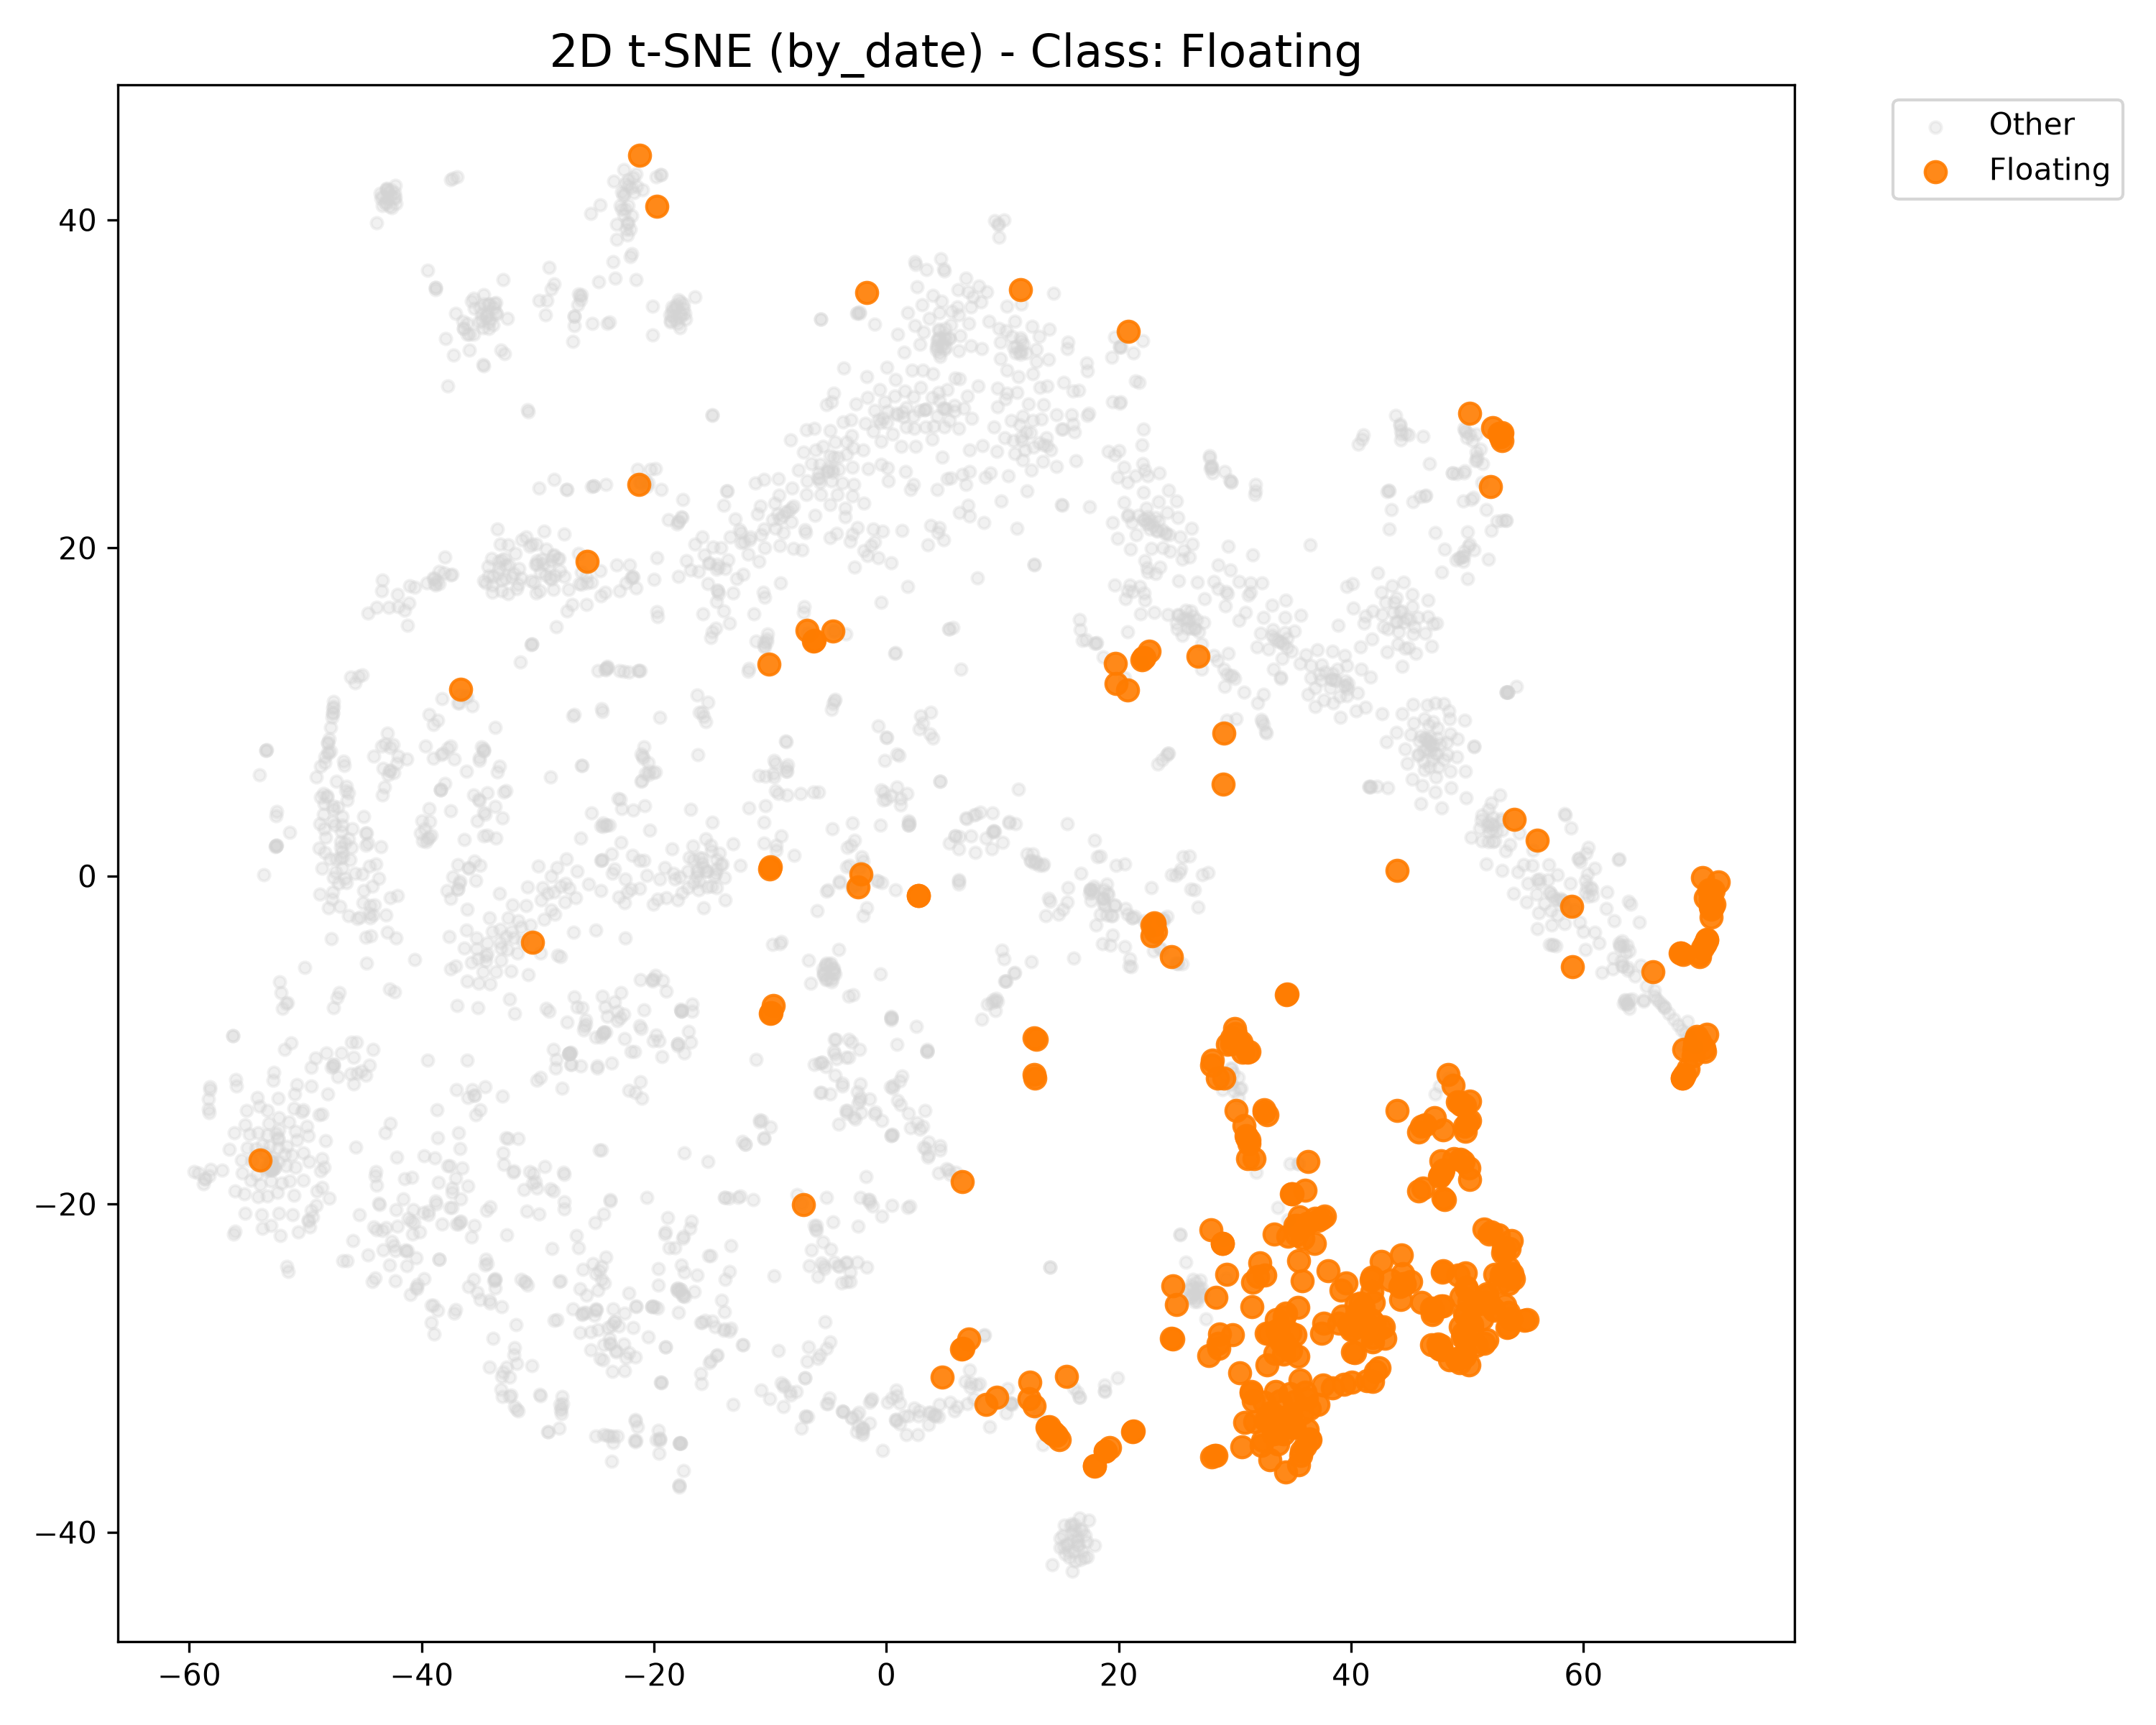
\includegraphics[width=\textwidth]{../Results/tsne_plots/data_by_date/split_2d_Floating.png}
        \caption{2D t-SNE: Floating}
    \end{subfigure}
    \hfill
    \begin{subfigure}[b]{0.45\textwidth}
        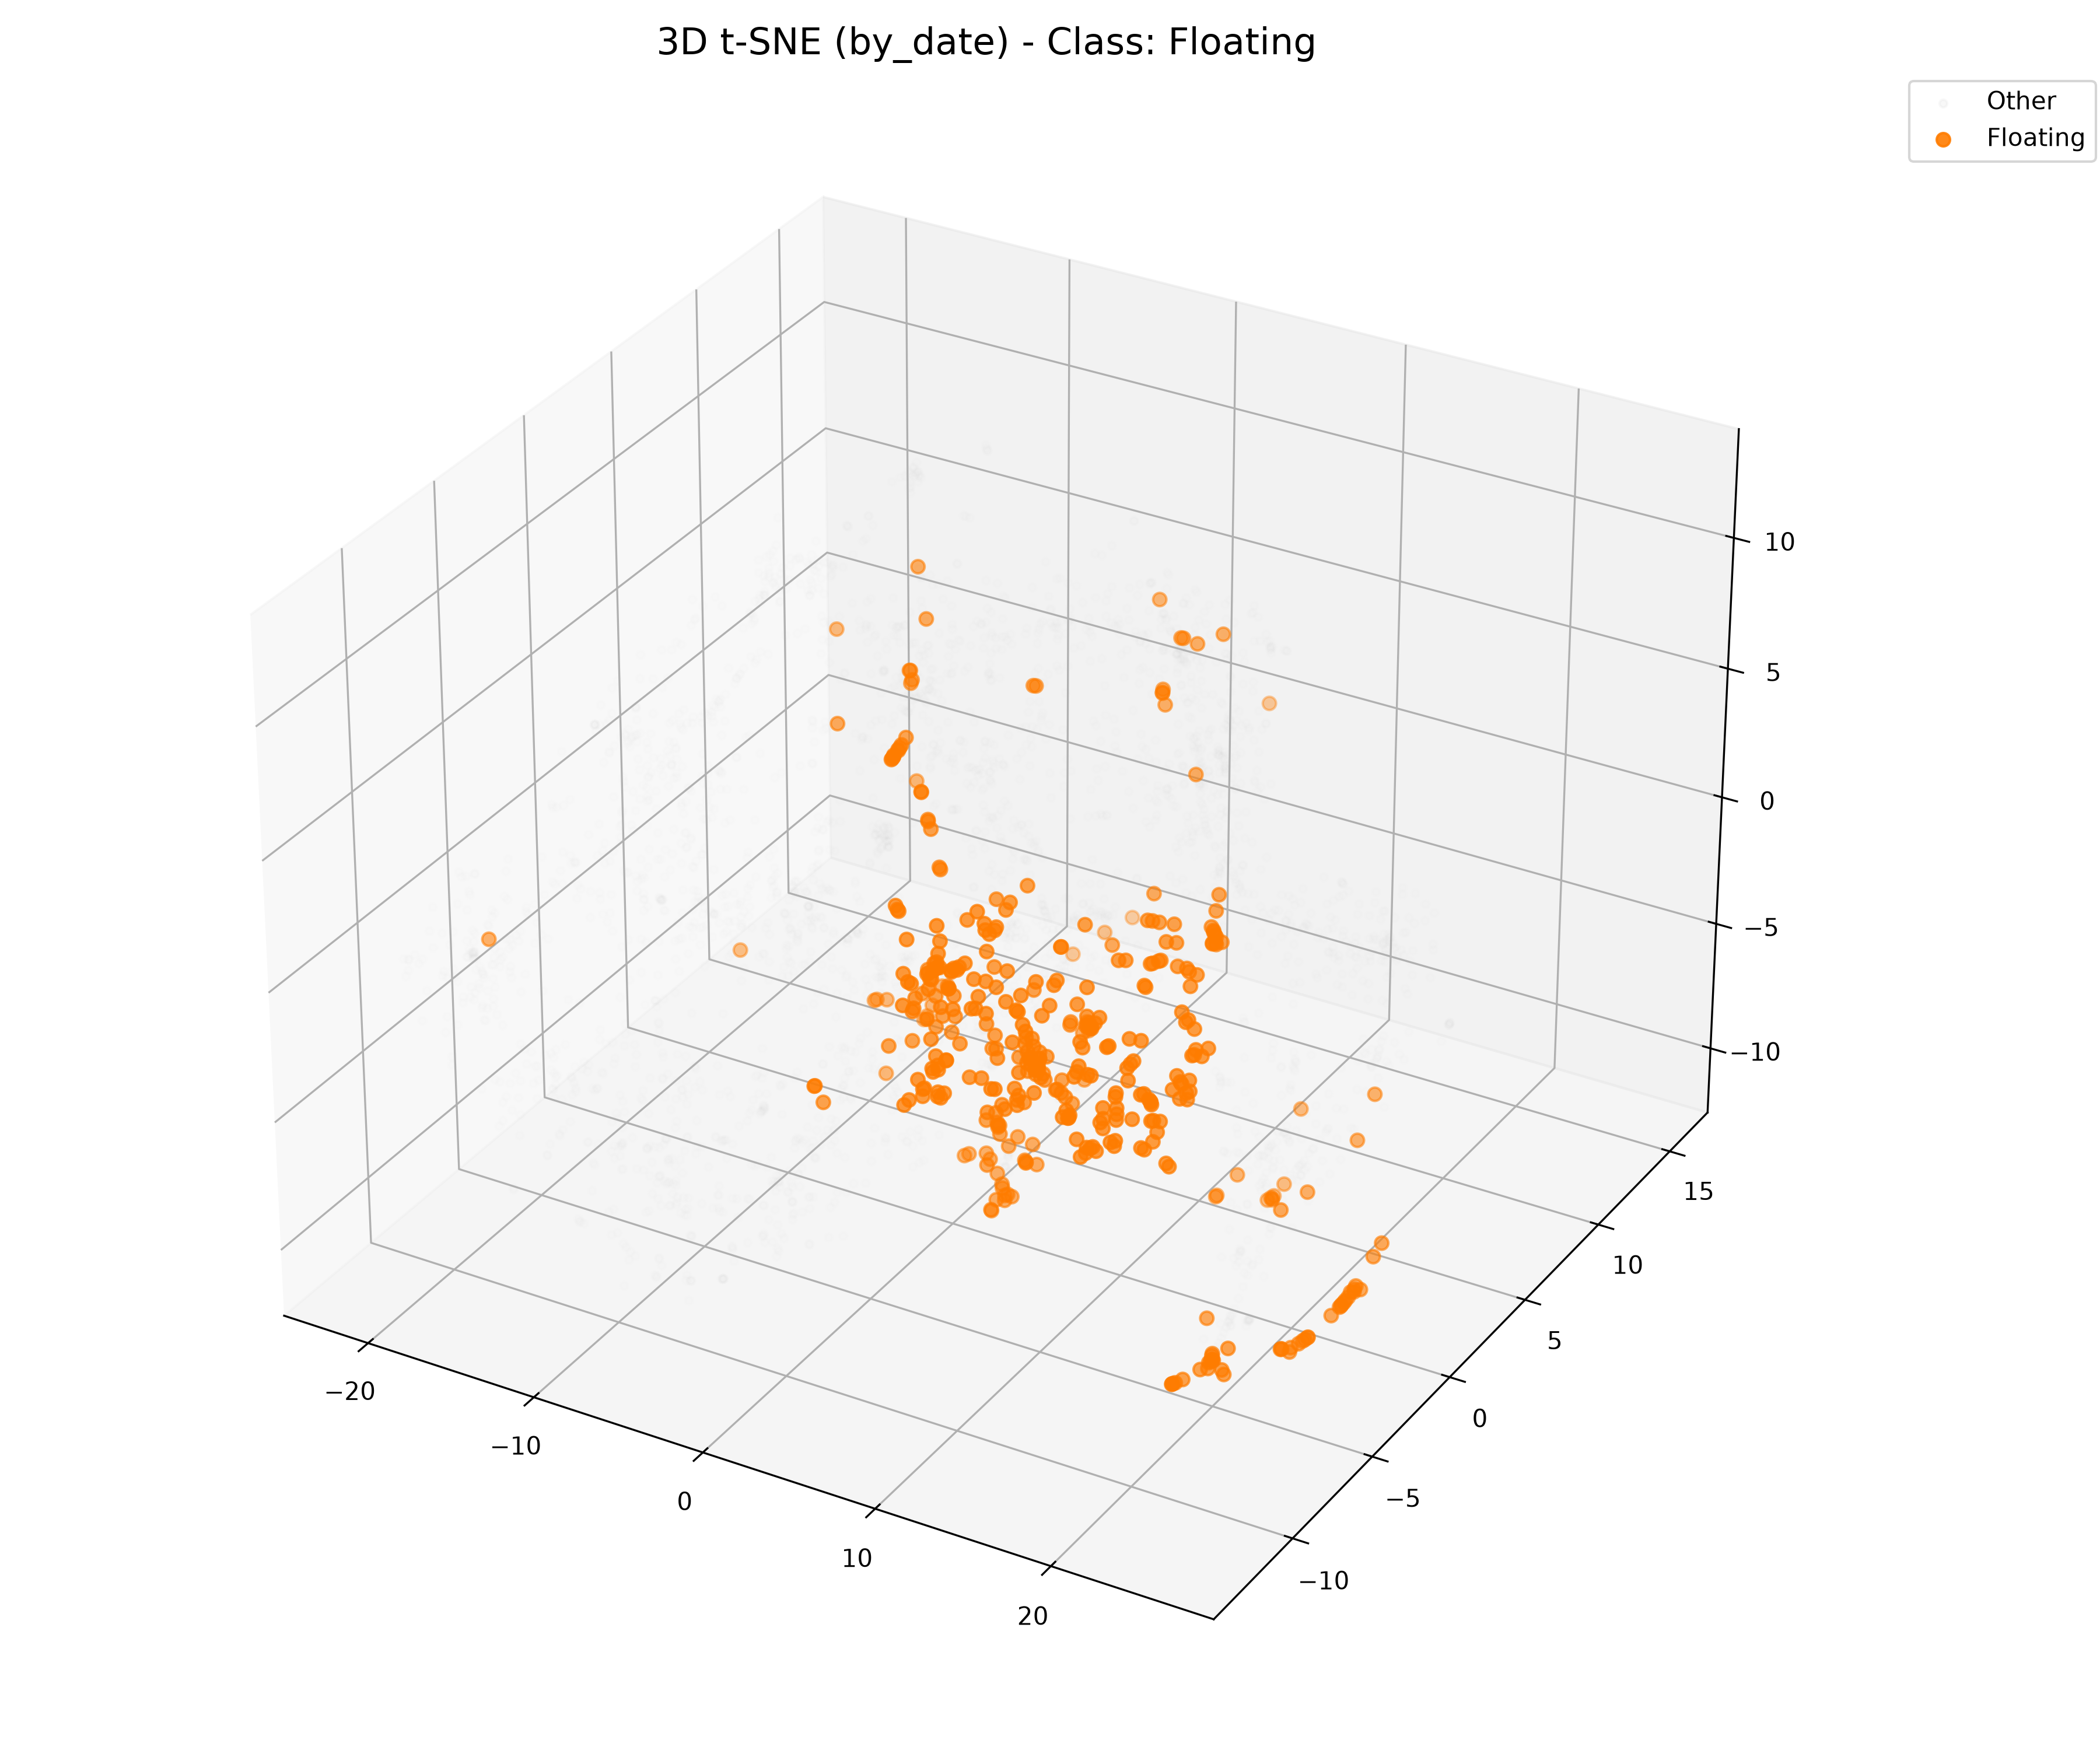
\includegraphics[width=\textwidth]{../Results/tsne_plots/data_by_date/split_3d_Floating.png}
        \caption{3D t-SNE: Floating}
    \end{subfigure}
    \caption{Highlighted distribution of Floating discharges within dated collections.}
\end{figure}

% Particle
\begin{figure}[H]
    \centering
    \begin{subfigure}[b]{0.45\textwidth}
        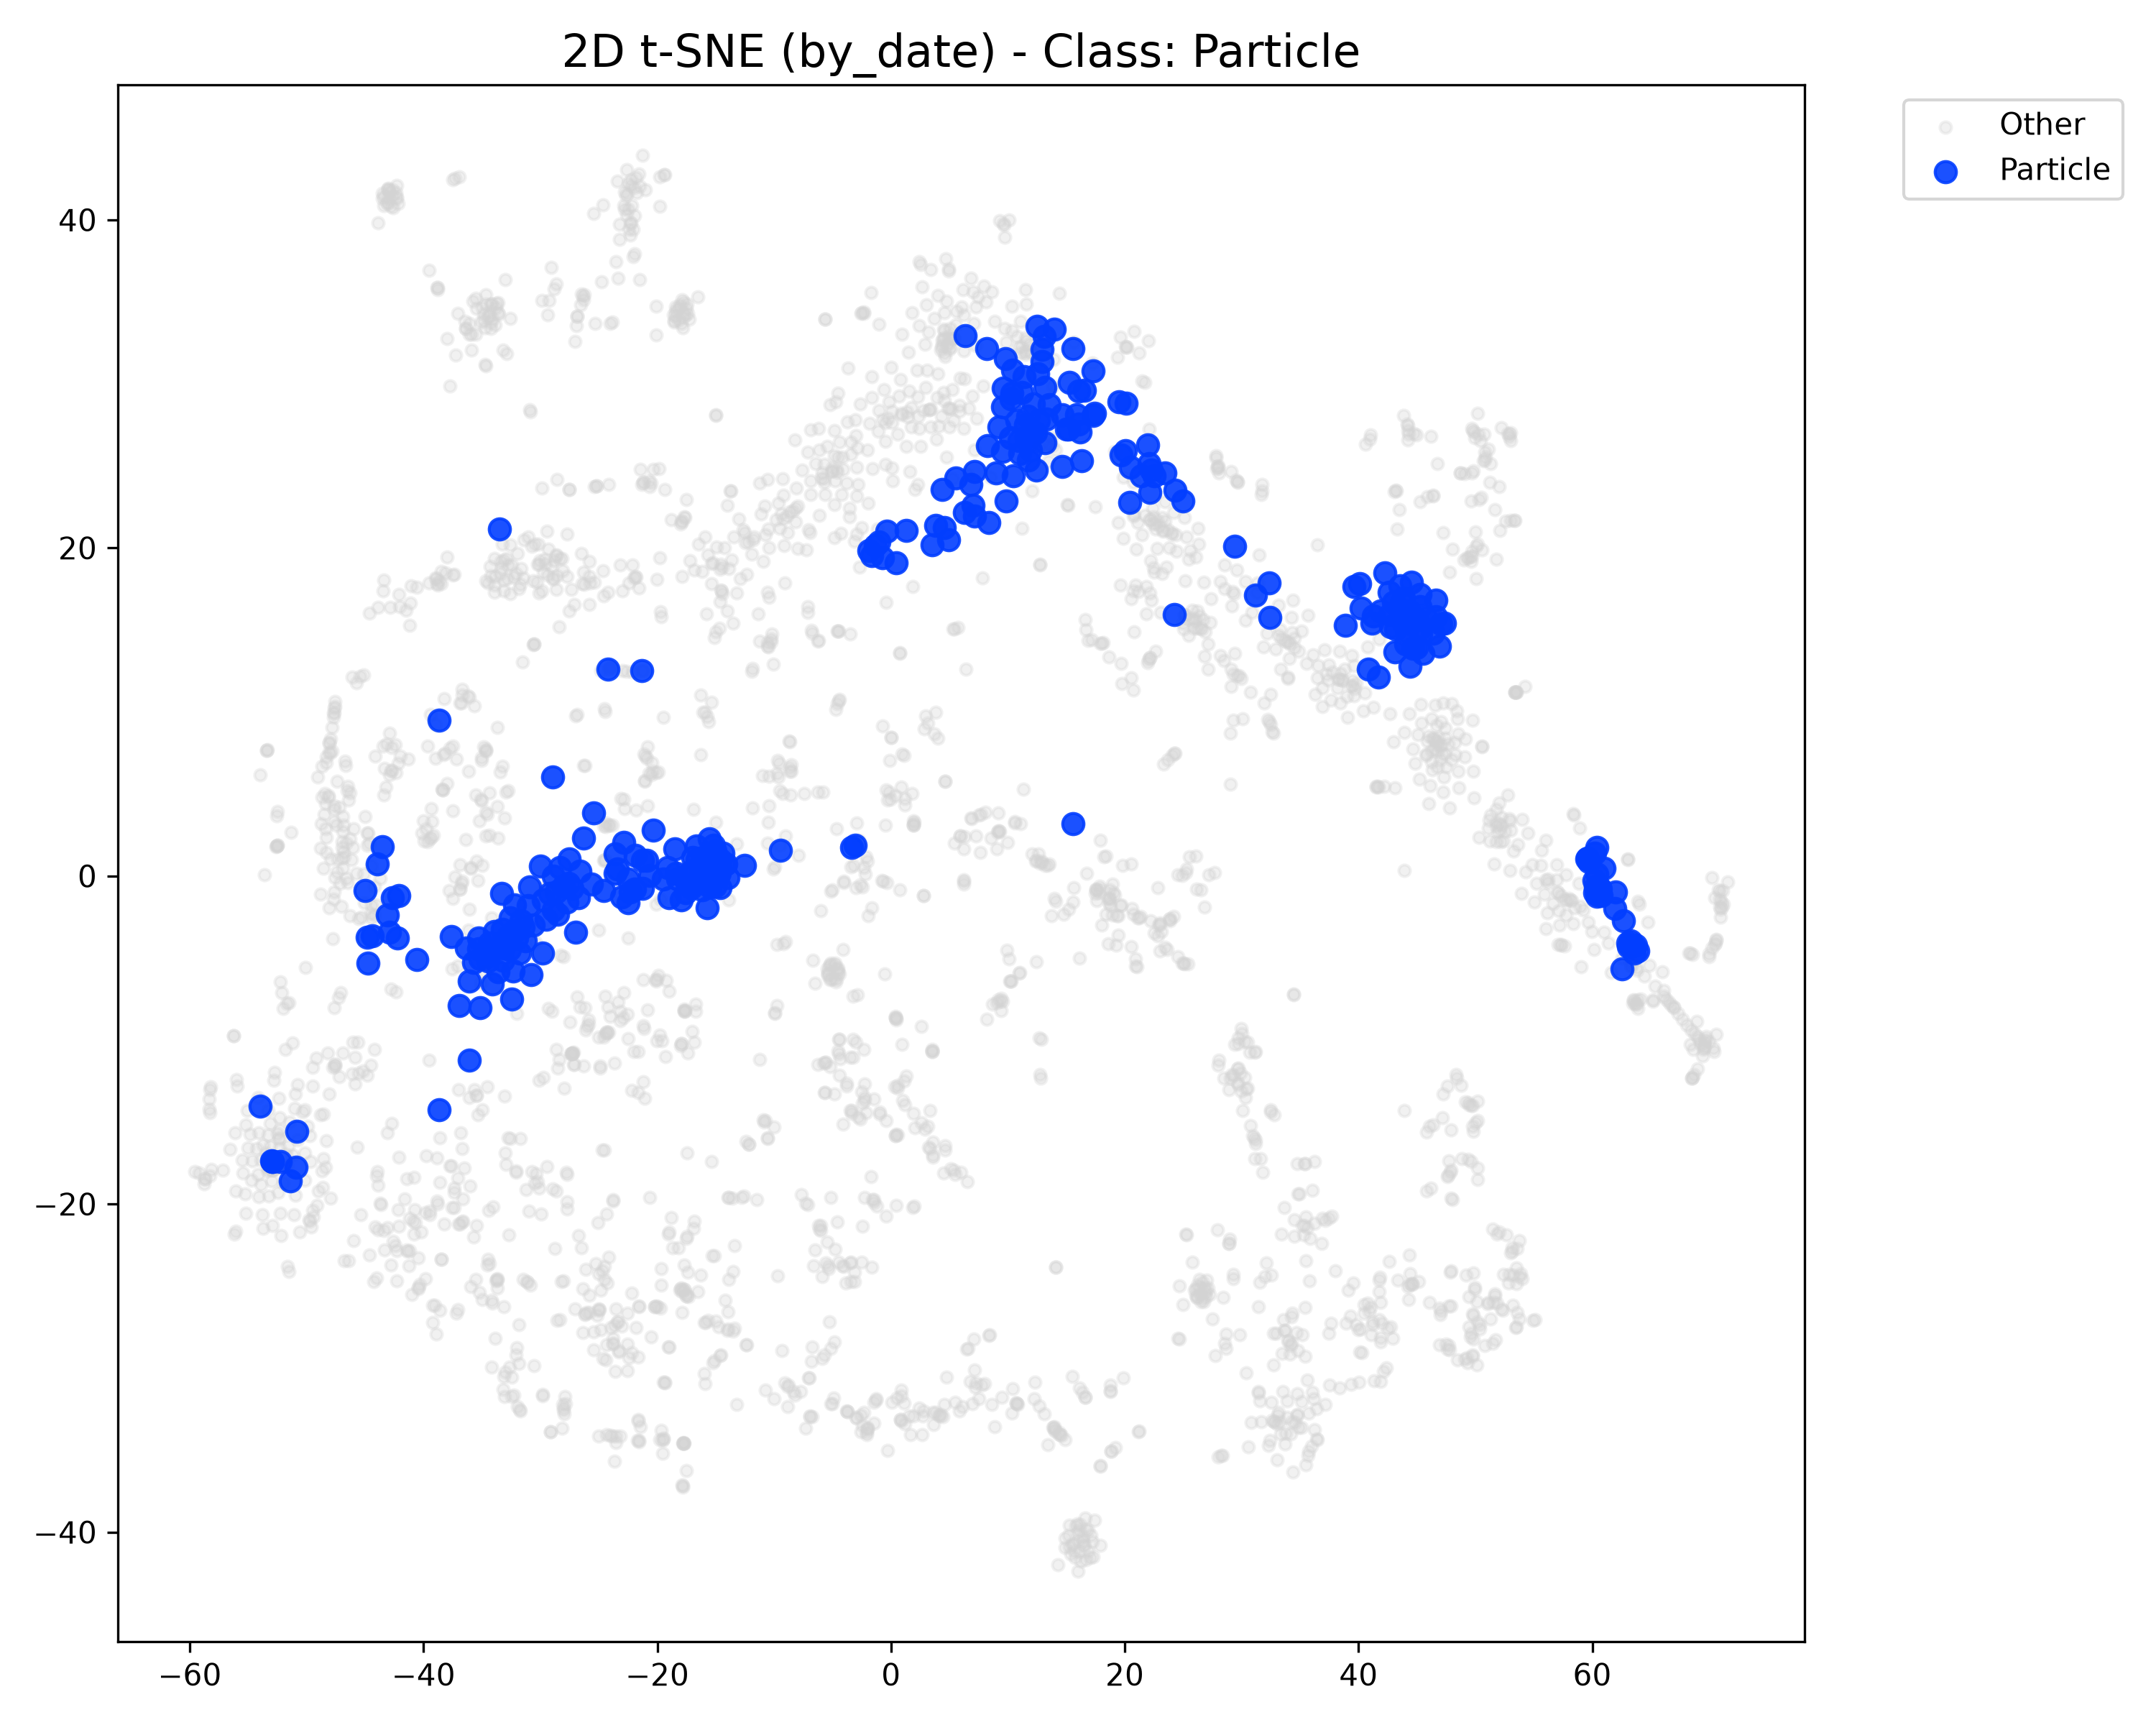
\includegraphics[width=\textwidth]{../Results/tsne_plots/data_by_date/split_2d_Particle.png}
        \caption{2D t-SNE: Particle}
    \end{subfigure}
    \hfill
    \begin{subfigure}[b]{0.45\textwidth}
        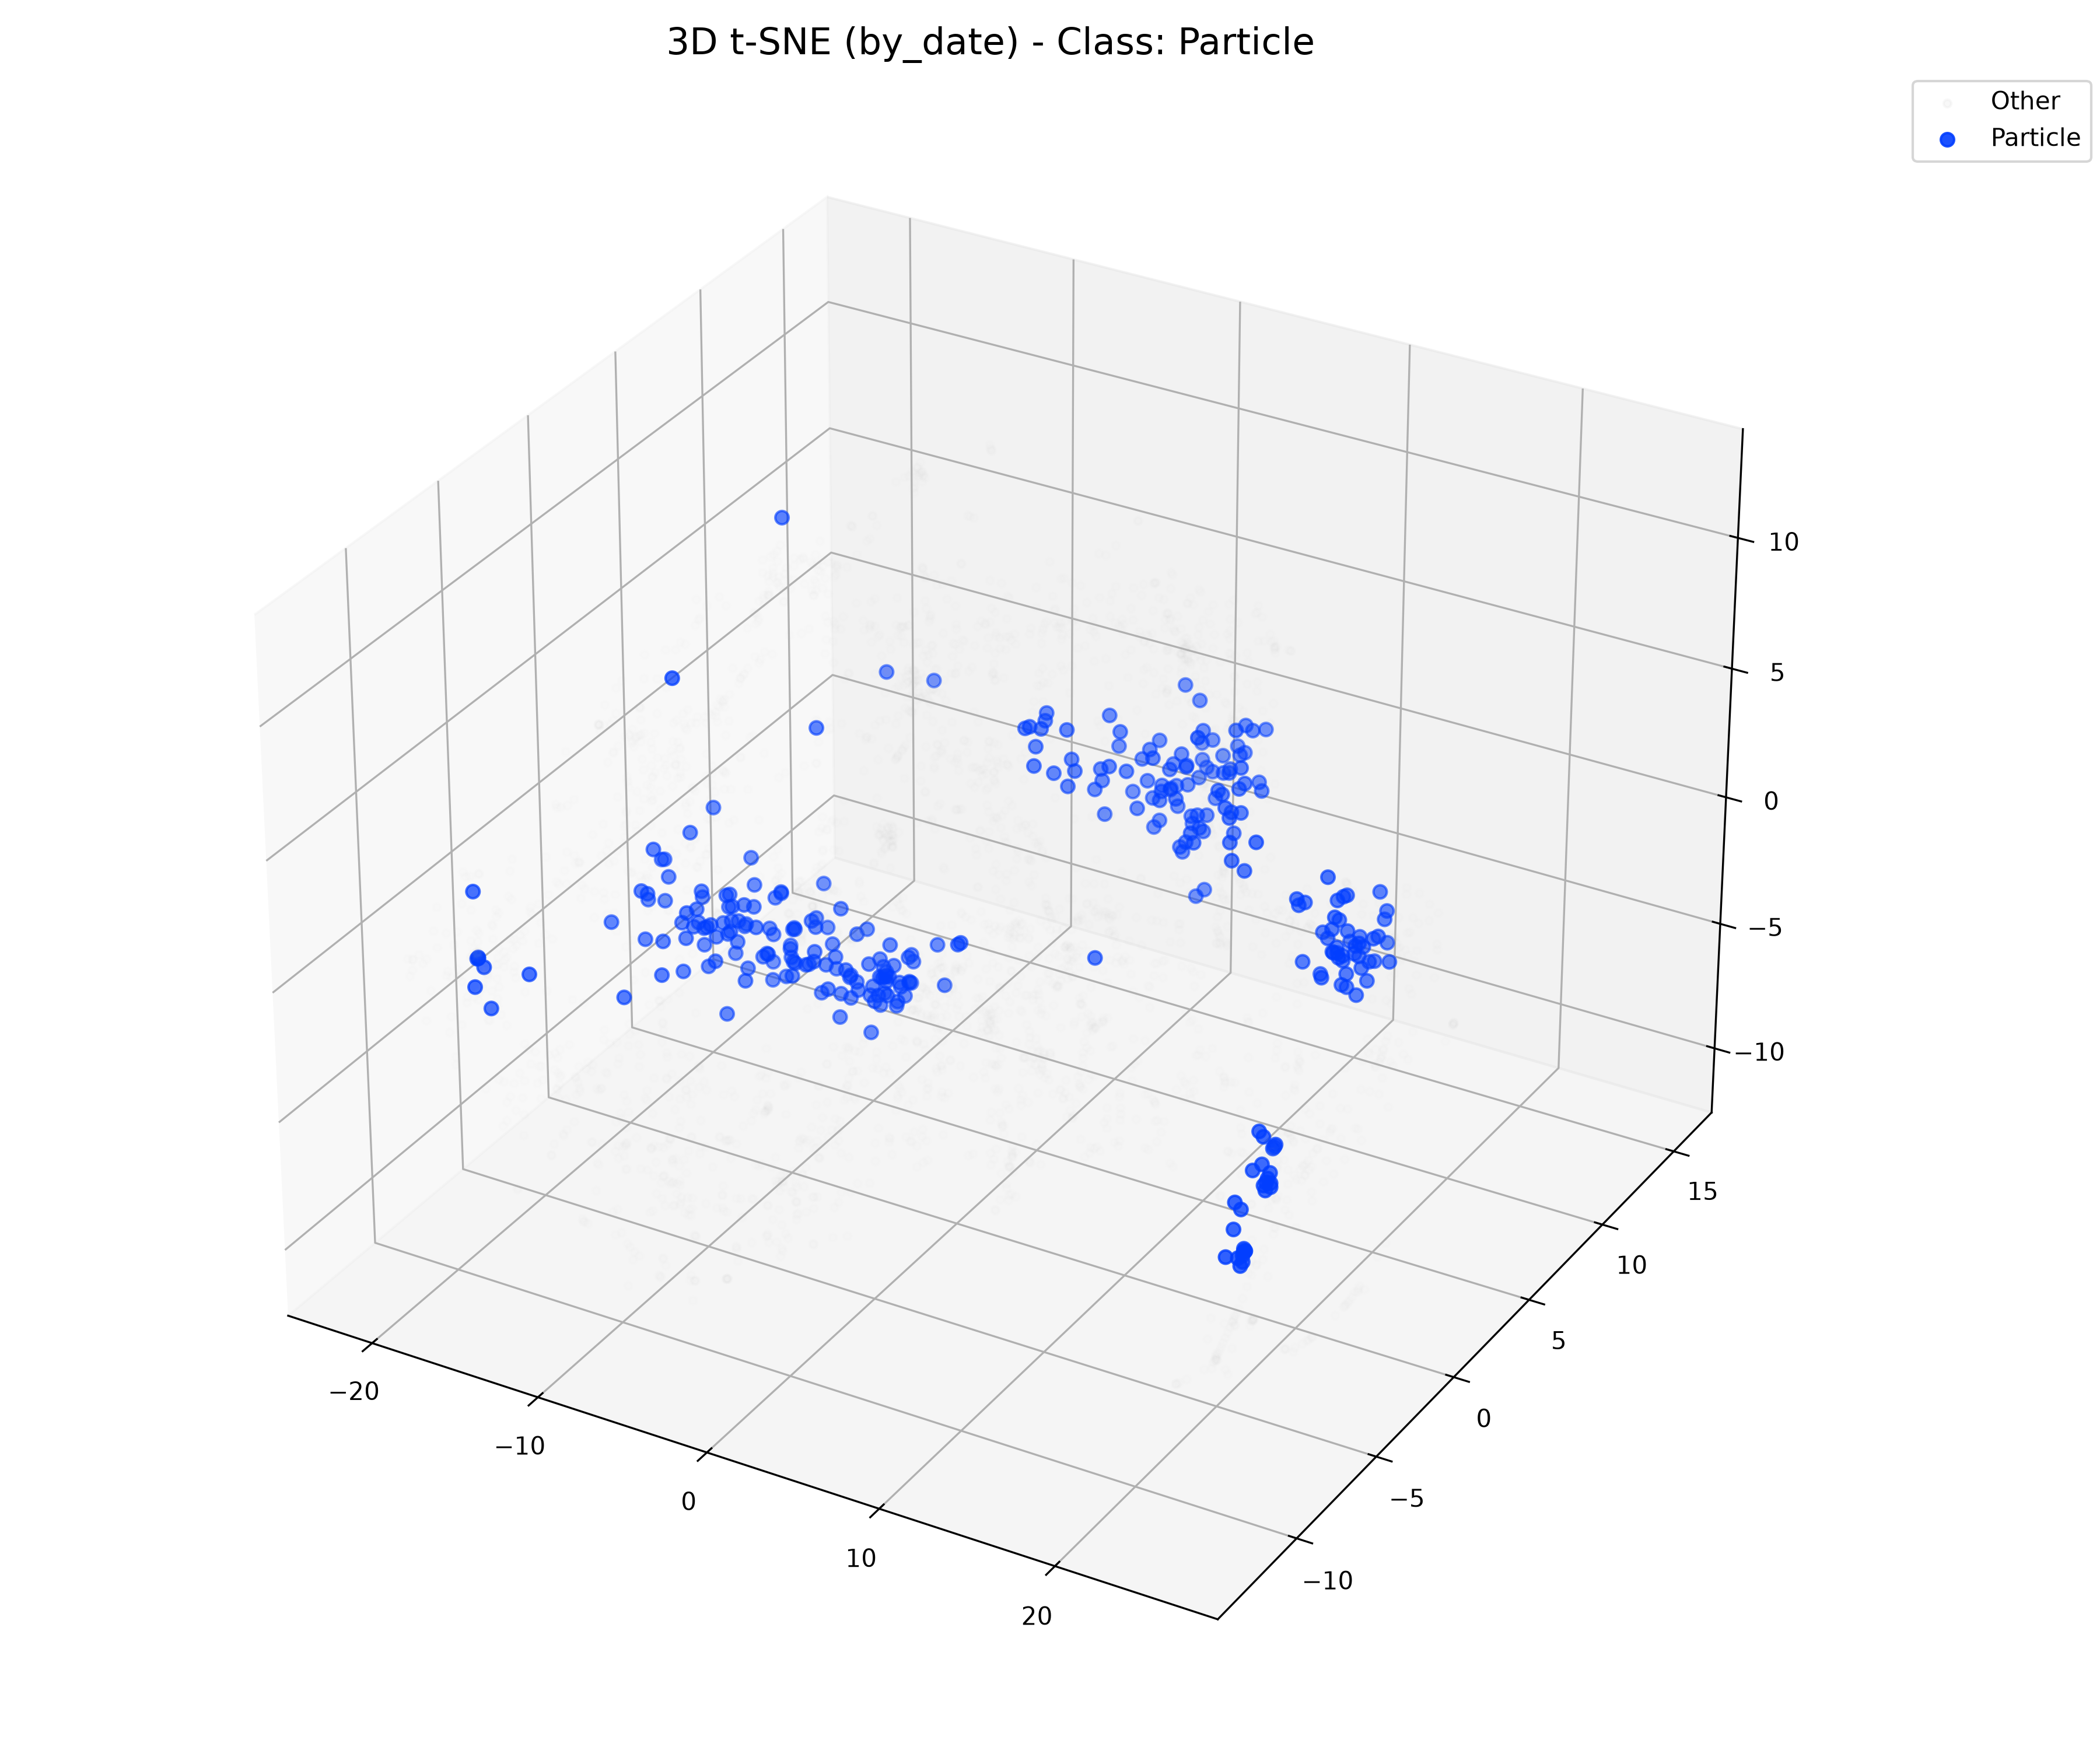
\includegraphics[width=\textwidth]{../Results/tsne_plots/data_by_date/split_3d_Particle.png}
        \caption{3D t-SNE: Particle}
    \end{subfigure}
    \caption{Highlighted distribution of Particle discharges within dated collections.}
\end{figure}

% Void
\begin{figure}[H]
    \centering
    \begin{subfigure}[b]{0.45\textwidth}
        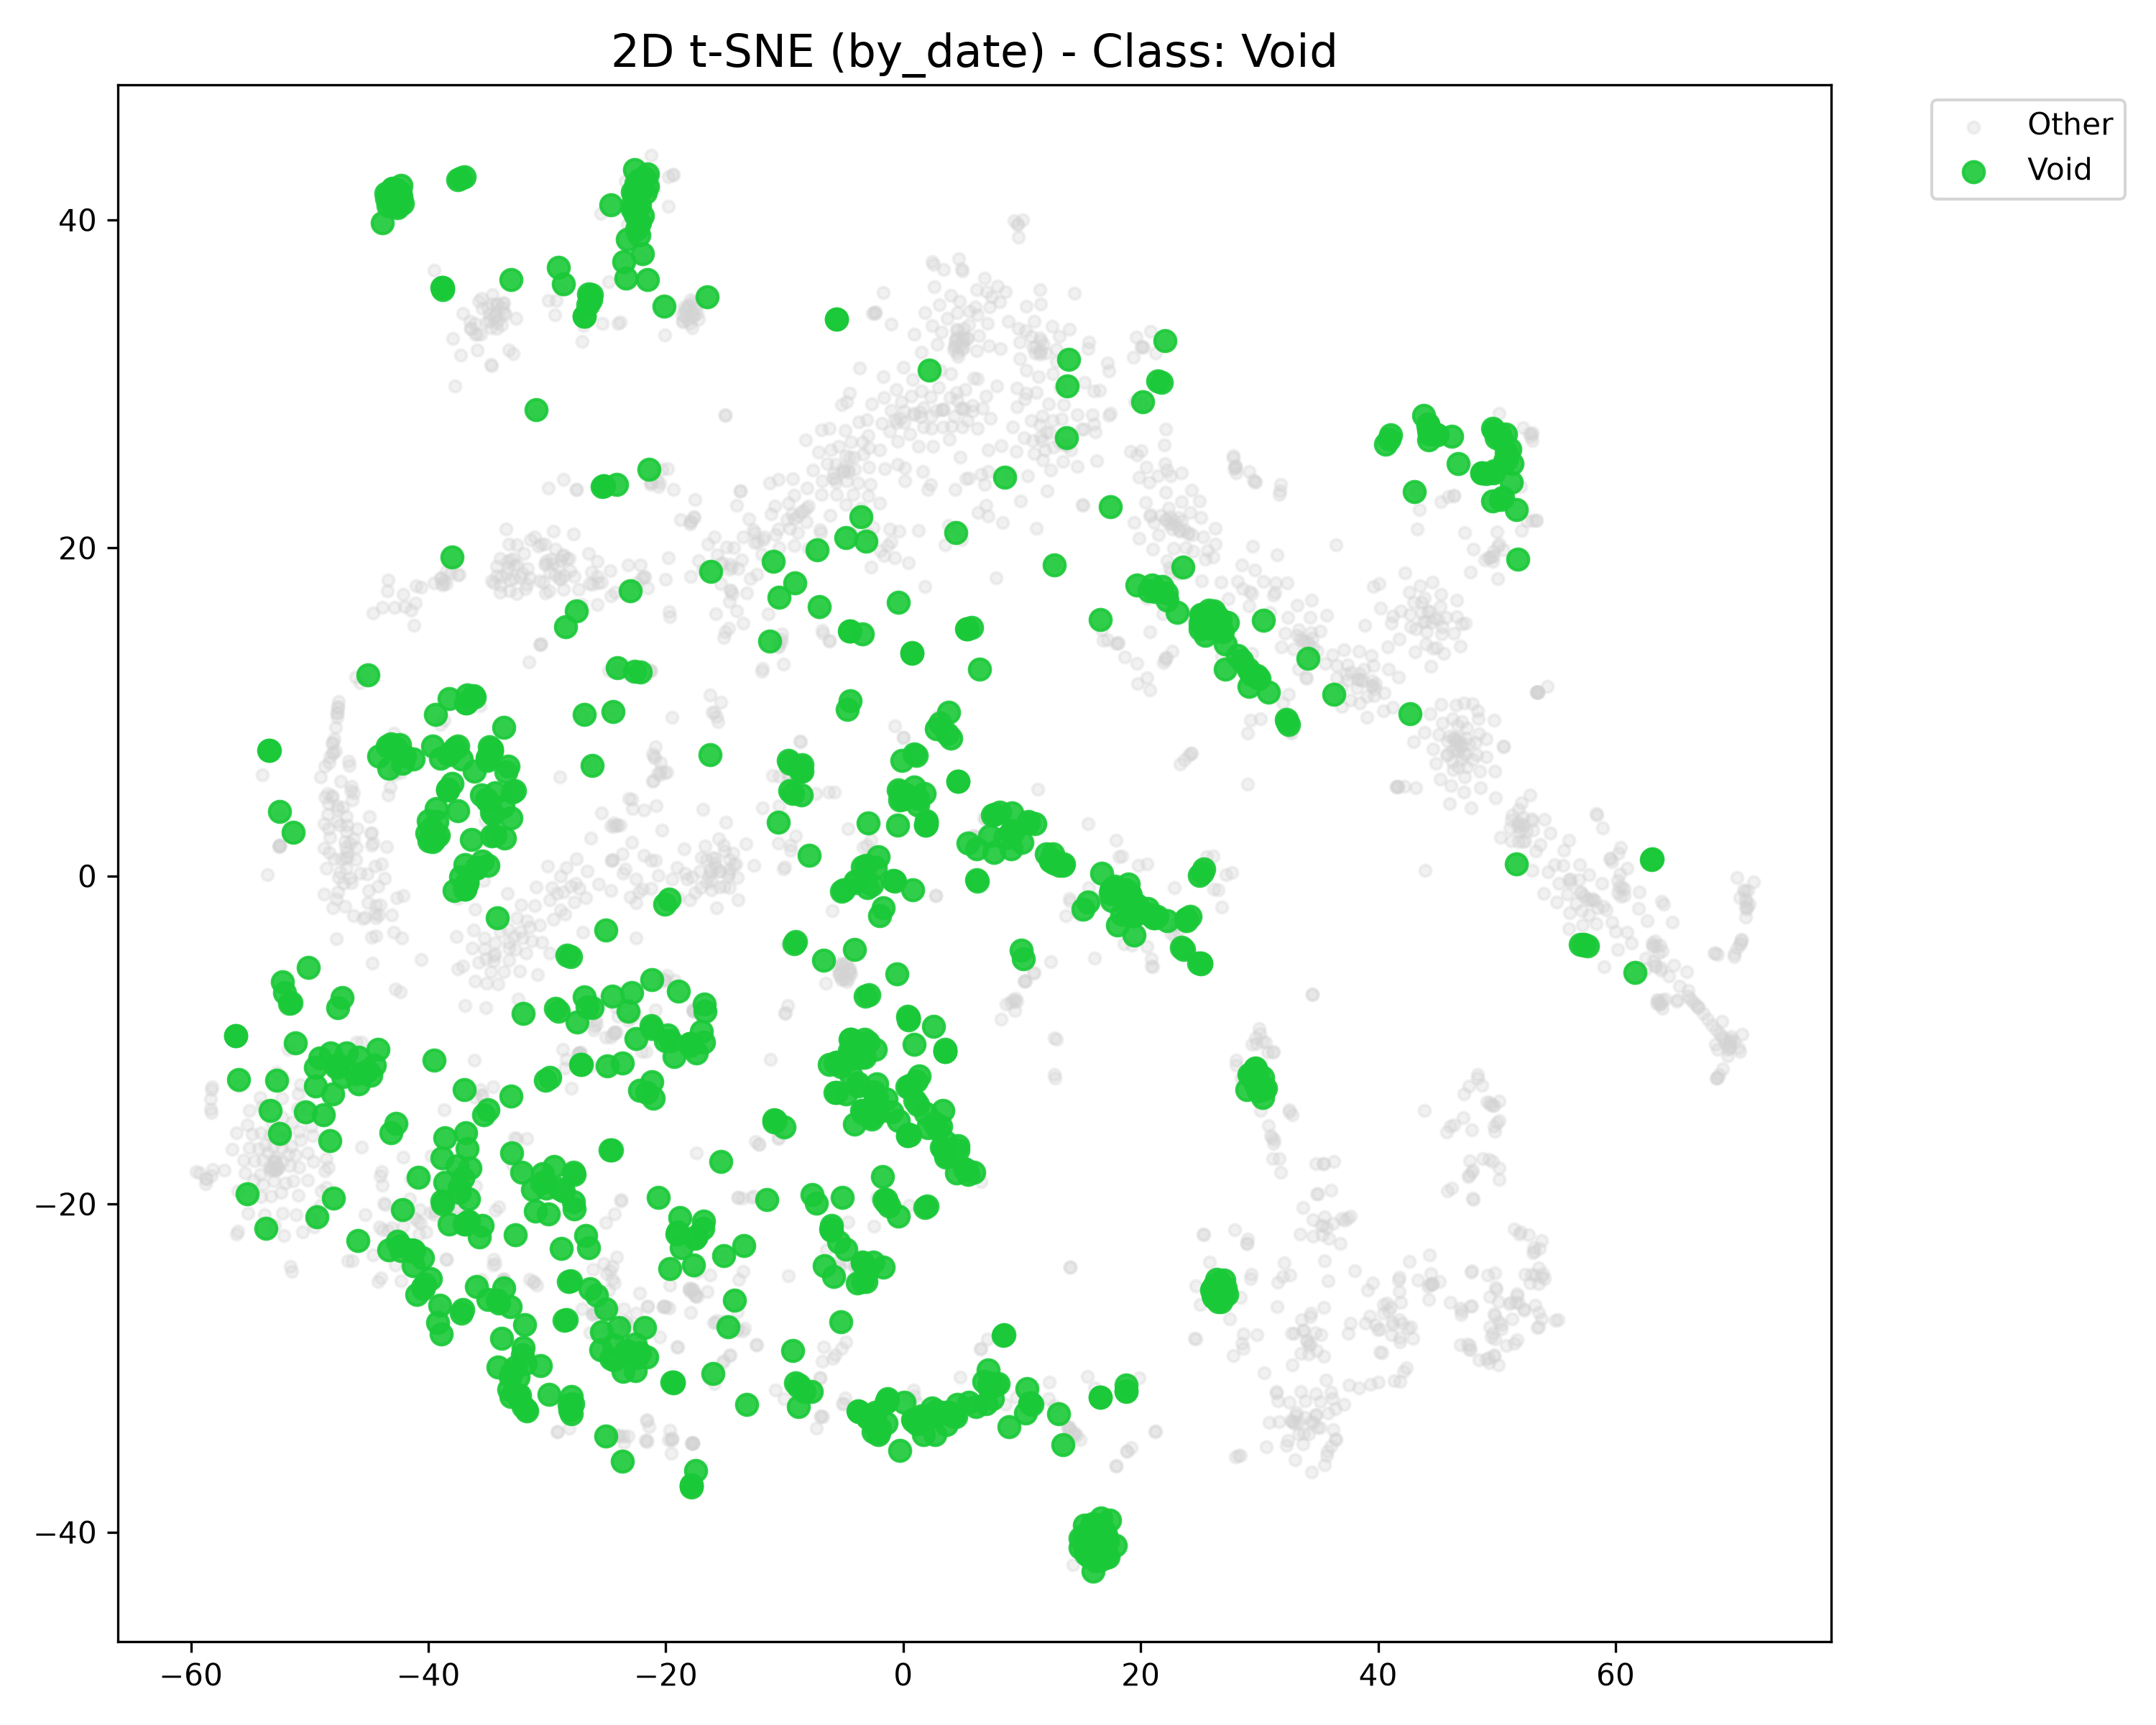
\includegraphics[width=\textwidth]{../Results/tsne_plots/data_by_date/split_2d_Void.png}
        \caption{2D t-SNE: Void}
    \end{subfigure}
    \hfill
    \begin{subfigure}[b]{0.45\textwidth}
        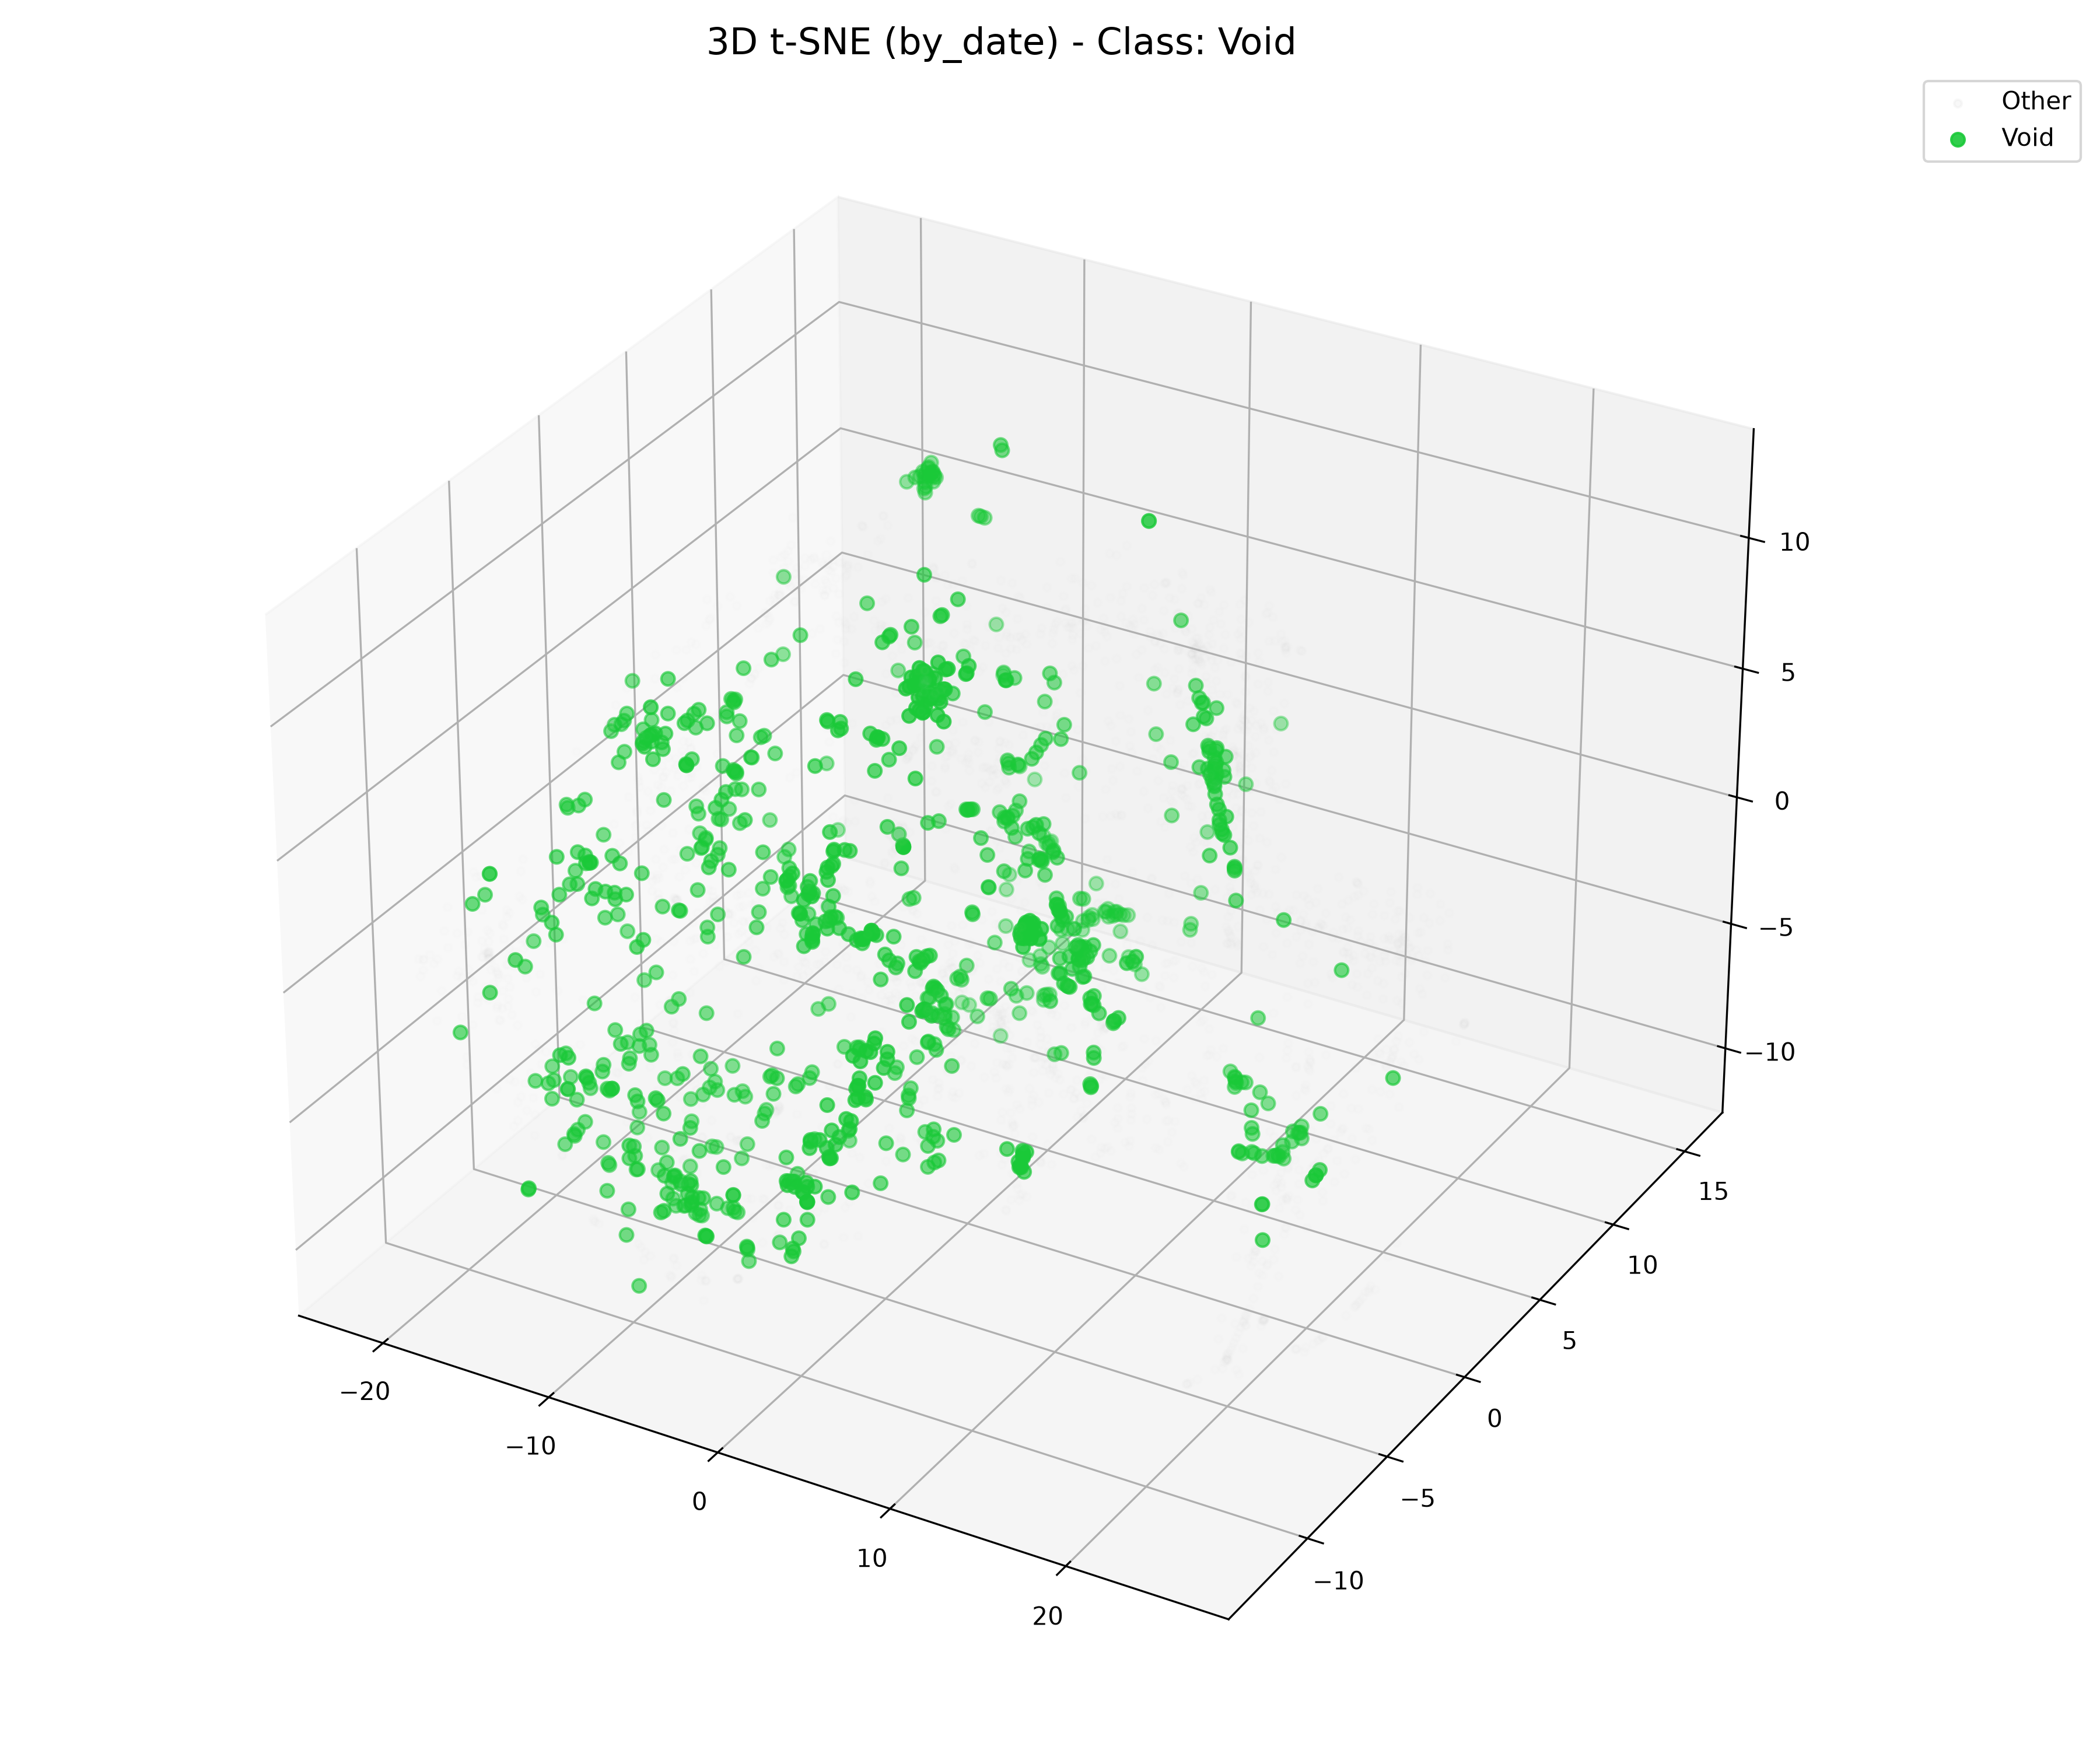
\includegraphics[width=\textwidth]{../Results/tsne_plots/data_by_date/split_3d_Void.png}
        \caption{3D t-SNE: Void}
    \end{subfigure}
    \caption{Highlighted distribution of Void discharges within dated collections.}
\end{figure}

% Noise
\begin{figure}[H]
    \centering
    \begin{subfigure}[b]{0.45\textwidth}
        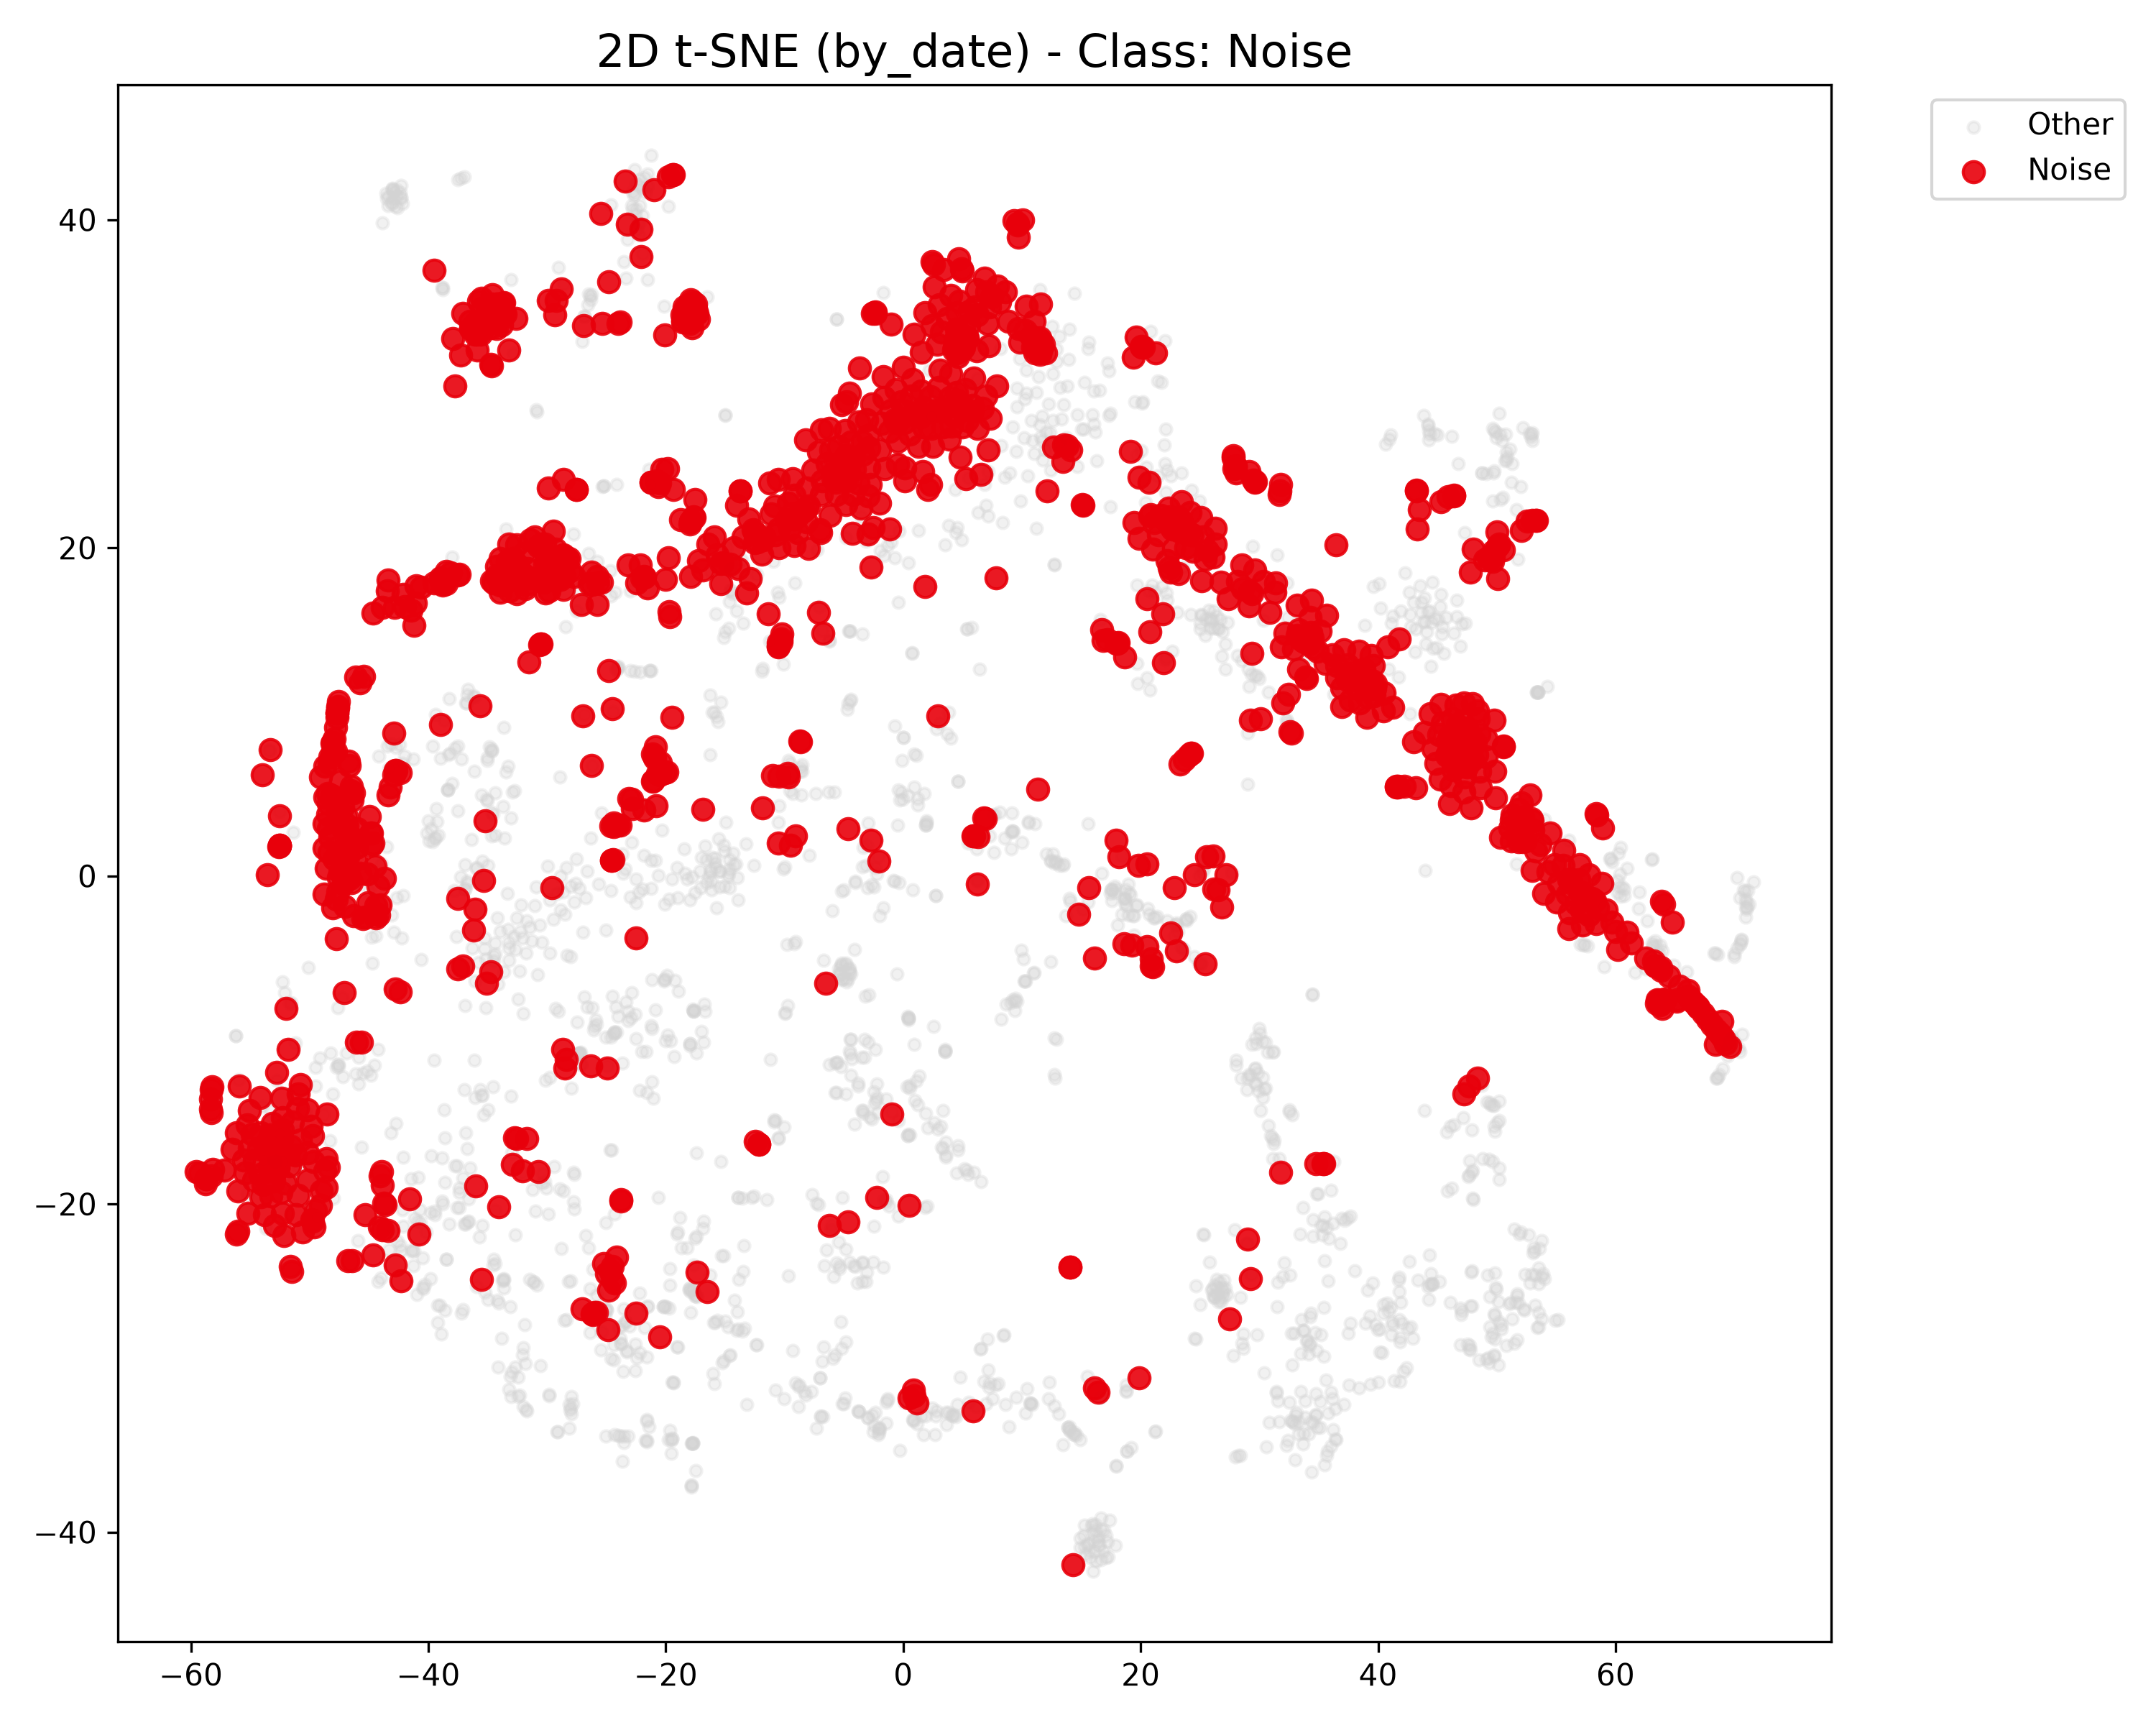
\includegraphics[width=\textwidth]{../Results/tsne_plots/data_by_date/split_2d_Noise.png}
        \caption{2D t-SNE: Noise}
    \end{subfigure}
    \hfill
    \begin{subfigure}[b]{0.45\textwidth}
        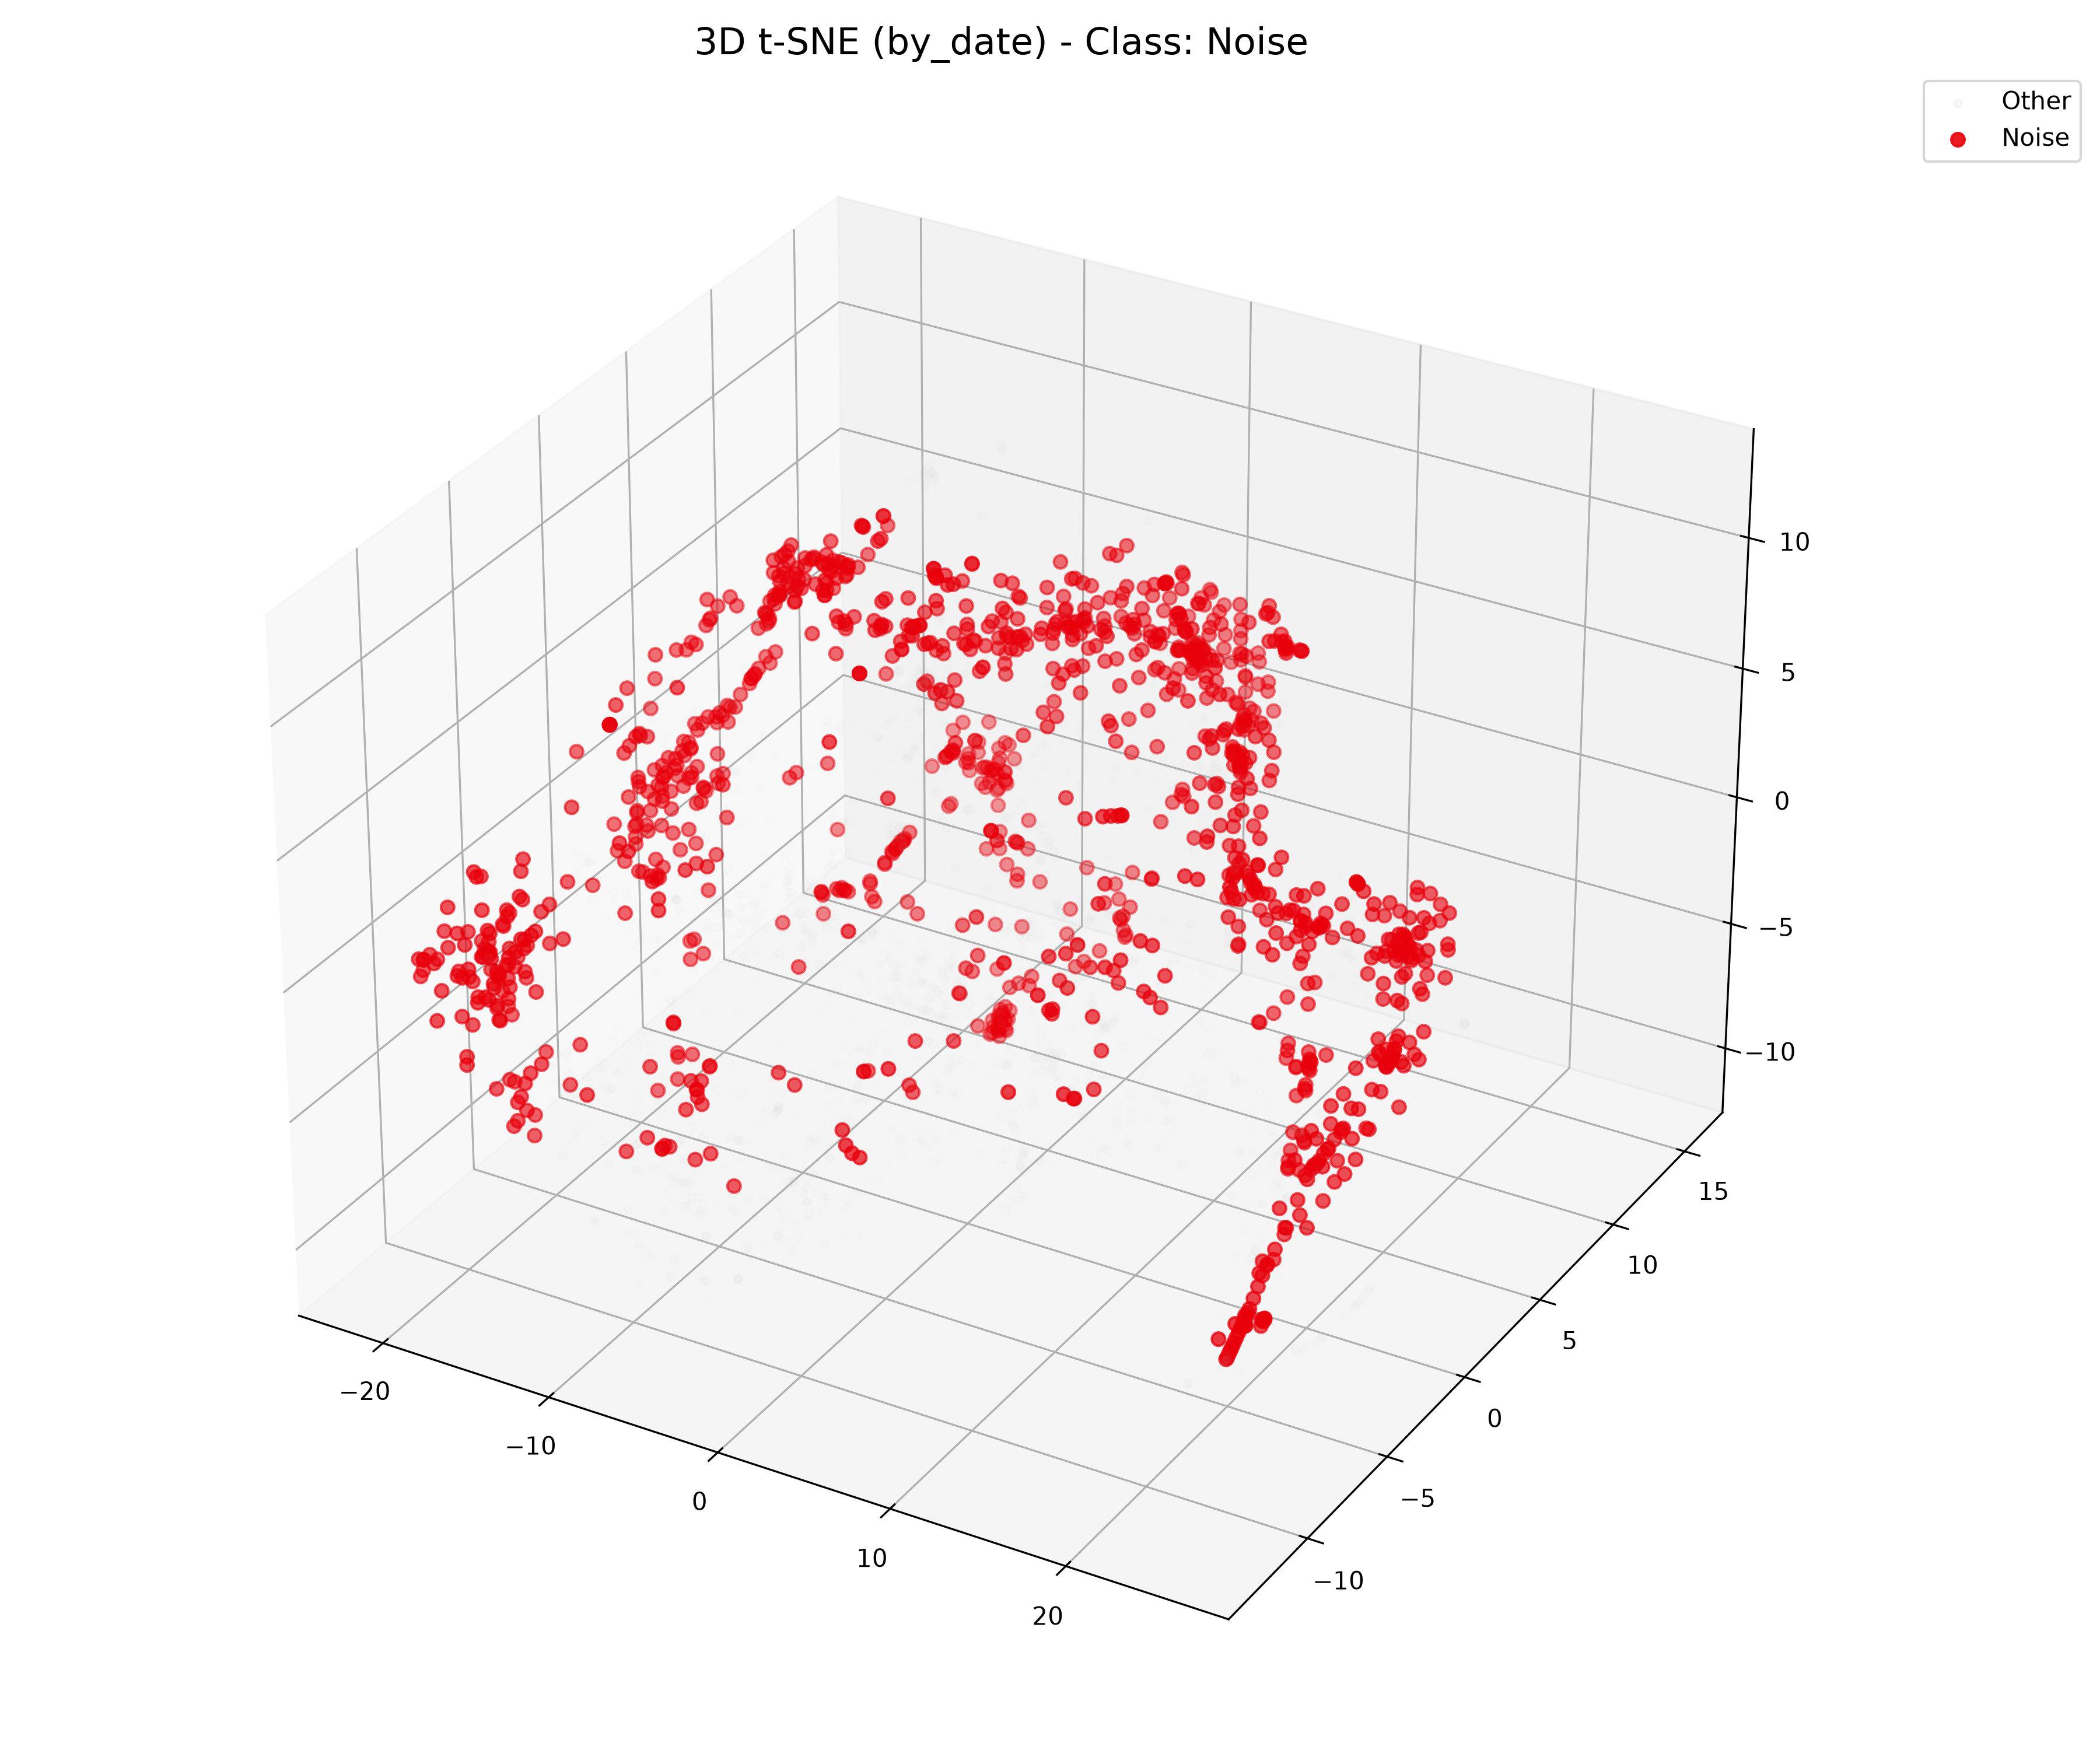
\includegraphics[width=\textwidth]{../Results/tsne_plots/data_by_date/split_3d_Noise.png}
        \caption{3D t-SNE: Noise}
    \end{subfigure}
    \caption{Highlighted distribution of Noise samples within dated collections.}
\end{figure}

\end{document}
